% PhD dissertation manuscript
% Started on: 18th Dec, 2014
% Draft completed on: Oct 23, 2015
% Saurav R Tuladhar

\documentclass[
12pt,
letterpaper,
% draft
]
{report}

\usepackage[noadjust]{cite}
\usepackage{hyperref}   % Generates bookmarks on pdf viewers
\usepackage{setspace}
\usepackage{amsmath}
\usepackage{amsfonts}
\usepackage{amssymb}
\usepackage[]{graphicx}
% \usepackage{fancyvrb}   % Fancy verbatim package 
% \usepackage{bm}
\usepackage{stmaryrd}
\usepackage{subfig}
\usepackage{algorithm}
\usepackage{algpseudocode}
\usepackage{ragged2e}
\usepackage[]{appendix}
\numberwithin{equation}{chapter}

\usepackage{titlesec}
\titleformat{\chapter}[display]{\normalfont\huge\bfseries\singlespacing}{\chaptertitlename\ \thechapter}{20pt}{\Huge}

\usepackage[titles, subfigure]{tocloft}
\usepackage{calc}

\renewcommand{\cftchappresnum}{Chapter }
\renewcommand{\cftchapaftersnum}{:}
\addtolength\cftchapnumwidth{\widthof{Chapter}}

% Letterpaper size: 8.27in x 11in
% % Margin reset---
\usepackage[top=1in, bottom=1.3in,
left=1.5in, right=1.1in,
footskip=0.3in]{geometry}

\graphicspath{{../figures/pdf/}}
\renewcommand{\figurename}{Fig.}

% Define \bstctlcite
\makeatletter
\def\bstctlcite{\@ifnextchar[{\@bstctlcite}{\@bstctlcite[@auxout]}}
\def\@bstctlcite[#1]#2{\@bsphack
 \@for\@citeb:=#2\do{%
   \edef\@citeb{\expandafter\@firstofone\@citeb}%
   \if@filesw\immediate\write\csname#1\endcsname{\string\citation{\@citeb}}\fi}%
 \@esphack}
\makeatother

\raggedbottom
% \onehalfspace
% Entry for title page
\author{Saurav R Tuladhar}
\title{PhD Dissertation Draft}
% \raggedright


\begin{document}

\bstctlcite{IEEEexample:BSTcontrol} % Control for IEEEtrans.bst to disable repeated name

% % -------------------Front Matter-----------------------
\setcounter{page}{1}
\pagenumbering{roman}  % Front matter needs to use roman page numbering

% Title page for PhD dissertation
% Saurav R. Tuladhar
% Oct 28, 2015

\thispagestyle{empty}
%\enlargethispage{0.8in} % default textheight is 592pt = 8.2inch
\newgeometry{margin=1.5in}
\doublespacing
\begin{center}

University of Massachusetts Dartmouth \\
College of Engineering \\


\vspace*{5em}
{\sc Improved Sample Matrix Inversion Adaptive Beamformers \\for Uniform Linear Arrays using Array Polynomial} \\

\vspace*{5em}
A Dissertation in 

Electrical Engineering 

by

Saurav R. Tuladhar 

\vspace*{7em}
Submitted in Partial Fulfillment of the 

Requirements for the Degree of \\ Doctor of Philosophy 

\vfill
January 2016

\end{center}
\restoregeometry
%%% Local Variables:
%%% mode: latex
%%% TeX-master: "main"
%%% End:

\clearpage

%Permission to UMassD
\thispagestyle{empty} %No page number
\doublespacing
\begin{flushleft}
I grant the University of Massachusetts Dartmouth the non-exclusive right to use
the work for the purpose of making single copies of the work available to the public
on a not-for-profit basis if the University's circulating copy is lost or destroyed.

\vskip 2em
\hfill \rule{2.73in}{0.5pt} \\
\vspace*{-0.5em}
\hspace*{3.17in}Saurav R. Tuladhar \\
\vspace{1em}
\hfill Date \rule{2.35in}{0.5pt} 
\end{flushleft}

%%% Local Variables:
%%% mode: latex
%%% TeX-master: "main"
%%% End:

\clearpage

\setcounter{page}{2}
% Signature page 
% Comment: use uniform units for length
\enlargethispage{3cm}
\newenvironment{changemargin}[2]{%
  \begin{list}{}{%
       \setlength{\textwidth}{6in} % 8.5 - 1.5 - 1 
       \setlength{\voffset}{0.5in}  % One inch + whatever set here
       \setlength{\marginparsep}{0in}
       \setlength{\topmargin}{0in}%
       \setlength{\headheight}{0in}
       \setlength{\headsep}{0in}
       \setlength{\footskip}{0in}
       \setlength{\footnotesep}{0in}
       \setlength{\rightmargin}{#2}%
       \setlength{\leftmargin}{#1}%
    }%
  \item[]}{\end{list}}
\thispagestyle{empty}
\newcommand{\titlesep}{0.15in}
\singlespacing
\begin{changemargin}{0in}{0in}
  \begin{flushleft}
    \normalsize
    We approve the dissertation of Saurav R. Tuladhar \par
    \vskip 0.05in
    \hspace{4.45in} Date of Signature
    \vskip 0.1in
    \rule{0.55\textwidth}{0.5pt} \hfill \rule{1.4in}{0.5pt} \\
    John R. Buck \\ Professor, Department of Electrical and Computer Engineering \\ Dissertation Advisor

    \vskip \titlesep    
    \rule{0.55\textwidth}{0.5pt} \hfill \rule{1.4in}{0.5pt} \\ 
    Dayalan P. Kasilingam \\ Professor, Department of Electrical and Computer Engineering \\ Dissertation Committee 
    
    \vskip\titlesep
    \rule{0.55\textwidth}{0.5pt} \hfill \rule{1.4in}{0.5pt} \\
    Paul J. Gendron \\ Assistant Professor, Department of Electrical and Computer Engineering \\ Dissertation Committee

    \vskip\titlesep
    \rule{0.55\textwidth}{0.5pt} \hfill \rule{1.4in}{0.5pt} \\
    Christ D. Richmond \\ Senior Technical Staff, MIT Lincoln Laboratory    \\ Dissertation Committee 

    \vskip\titlesep
    \rule{0.55\textwidth}{0.5pt} \hfill \rule{1.4in}{0.5pt} \\
    Raj R. Nadakuditi \\ Assistant Professor, University of Michigan \\ Dissertation Committee 

    \vskip \titlesep
    \rule{0.55\textwidth}{0.5pt} \hfill \rule{1.4in}{0.5pt} \\
    Hong Liu \\ Graduate Program Director\\ Department of Electrical and Computer Engineering 
    
    \vskip \titlesep
    \rule{0.55\textwidth}{0.5pt} \hfill \rule{1.4in}{0.5pt} \\
    Antonio H. Costa \\ Chairperson, Department of Electrical and Computer Engineering  

    \vskip \titlesep
    \rule{0.55\textwidth}{0.5pt} \hfill \rule{1.4in}{0.5pt} \\
    Robert E. Peck \\ Dean, College of Engineering 

    \vskip \titlesep
    \rule{0.55\textwidth}{0.5pt} \hfill \rule{1.4in}{0.5pt} \\
   Tesfay Meressi\\
   Associate Provost for Graduate Studies

  \end{flushleft}

\end{changemargin}
\clearpage
%%% Local Variables:
%%% mode: latex
%%% TeX-master: "main"
%%% End:

\clearpage


\newgeometry{top=0in}
\onehalfspacing
\chapter*{Abstract}
Analysis and Design of Adaptive Beamformers using Array Polynomial
\begin{flushleft}
by Saurav R. Tuladhar \\
\end{flushleft}

Adaptive beamformers (ABFs) place deep beampattern notches near
interferers to suppress the interferers’ power in the ABF output. The
sample matrix inversion (SMI) Minimum Variance Distortionless Response
(MVDR) ABF computes the beamformer weights by substituting the sample
covariance matrix (SCM) for the unknown ensemble covariance matrix in
the MVDR expression. Errors in the SCM estimate of interferer
direction due to limited sample support or interferer motion distorts
the ABF beampattern and degrades the ability of the ABF to suppress
the interferer. For beamformers using uniform linear arrays (ULA), the
beampattern can be represented as a polynomial. The array polynomial
is the $z$-transform of the beamformer weights. Evaluating the array
polynomial on the unit circle in the complex plane yields the
beampattern. For the ensemble MVDR beamforming using a ULA, the array
polynomial zeros are constrained to fall on the unit circle. But the
SMI MVDR polynomial zeros generally do not fall on the unit
circle. The first part of the dissertation develops a model for the
ensemble MVDR polynomial zero locations assuming a single interferer
present in white background noise. The model illuminates the trade off
balancing the interferer suppression and the white noise gain by the
ensemble MVDR. Secondly, the dissertation proposes the unit circle
MVDR (UC MVDR) beamformer which projects the SMI MVDR polynomial zeros
radially on to the unit circle to satisfy the constraint on the zeros
of ensemble MVDR polynomial. Numerical simulations show that the UC
MVDR beamformer suppresses interferers better than the SMI MVDR and
diagonal loaded MVDR beamformer and also improves the white noise gain
(WNG). Finally, the dissertation proposes the double zero (DZ) MVDR
ABF as a new approach to notch broadening. The array polynomial for
the DZ MVDR ABF has second-order zeros, producing broader and deeper
notches in the interferer direction. The DZ MVDR ABF outperforms the
SMI MVDR and covariance matrix tapered ABFs in simulations with
stationary and moving interferers.

\restoregeometry

%%% Local Variables:
%%% mode: latex
%%% TeX-master: "main"
%%% End:

\clearpage
% by Saurav Ratna Tuladhar \newline

\doublespacing
\chapter*{Acknowledgments}
The true flavor, the real fun, the continuous excitement of work lie in the process of doing it rather than in having it over and done with. - The Wings of Fire.

I would like to thank all who have assisted and supported me through my research and the thesis compilation process.

I am especially thankful to Dr.~John R. Buck, my advisor, for his continual guidance throughout my research. He has always pushed me for improvement through his subtle encouragements and appreciations. As a result I feel prepared to undertake future research endeavors. 

I would also like to thank my lab colleagues Dave, Peter, Sudeep and Kaushallya who were always willing to listen to my research ideas and discuss possible solution approaches.

I am thankful to my parents, Sugat my brother, Matina my wife and all family members back home who have supported me all the way through this process. I always found myself filled with new energy after talking with family members during weekends. Their support has been an essential impetus for me during my research days.

I am also thankful to all the staff members of Department of Electrical and Computer Engineering for their help on administrative tasks. Finally I would like to acknowledge Office of Naval Research (ONR) for funding my PhD research.

%%% Local Variables:
%%% mode: latex
%%% TeX-master: "main"
%%% End:

\clearpage

% Table of contents
\renewcommand\cftchapfont{\normalfont}
\renewcommand\cftchappagefont{\normalfont}
\renewcommand{\contentsname}{Table of contents}
\singlespacing
\setcounter{tocdepth}{2}
\tableofcontents
\clearpage 

% List of figures
\setlength{\cftfigindent}{0em}
% disable spacing between figure groups belonging to a chapter
%\newcommand*{\noaddvspace}{\renewcommand*{\addvspace}[1]{}} 
%\addtocontents{lof}{\protect\noaddvspace}
\renewcommand{\listfigurename}{List of figures}
\addcontentsline{toc}{chapter}{\listfigurename{}}
\listoffigures



% \addcontentsline{toc}{chapter}{List of Tables}
% \listoftables
% \newpage 

% --------- End of Front Matter---------------------------------

% ---------- Start of Chapters----------------------------------
\clearpage
\doublespacing
\thispagestyle{plain}
\setcounter{page}{1}
\pagenumbering{arabic}

% Main body
%Command shortcuts for various math symbols
% Inherited from JRB and KEW
\newcommand{\Cov}{\boldsymbol{\Sigma}}
\newcommand{\cov}{\sigma}
\newcommand{\Covdmr}{\Cov_{\rm DMR}}
\newcommand{\eval}{\gamma}
\newcommand{\Eval}{\boldsymbol{\Gamma}}
\newcommand{\evec}{\boldsymbol{\xi}}
\newcommand{\Evec}{\boldsymbol{\Xi}}
\newcommand{\sampCov}{{\bf S}}
\newcommand{\sampcov}{s}
\newcommand{\sampCovdmr}{\sampCov_{\rm DMR}}
\newcommand{\sampeval}{g}
\newcommand{\sampEval}{{\bf G}}
\newcommand{\sampevec}{{\bf e}}
\newcommand{\sampEvec}{{\bf E}}
\newcommand{\herm}{^{\rm H}}
\newcommand{\trans}{^{\rm T}}
\newcommand{\rep}{{\bf v}}        % planewave replica
\newcommand{\repmat}{{\bf V}}     % replica matrix
\newcommand{\sigamp}{b}
\newcommand{\wmvdr}{{\bf w}_{\rm MVDR}}
\newcommand{\wdmr}{{\bf w}_{\rm DMR}}
\newcommand{\dl}{\delta}
\newcommand{\dlmin}{\dl_{min}}
\newcommand{\wconv}{{\bf w}_{\rm conv}}
\newcommand{\nulldepth}{\mbox{ND}}
\newcommand{\replook}{\rep_0}
\newcommand{\repint}{\rep_I}
\newcommand{\tsp}{^{\rm T}}
\newcommand{\inv}{^{-1}}
\newcommand{\limrmt}{\lim_{RMT}}
\newcommand{\eig}{\operatorname{eig}}
\newcommand{\diag}{\operatorname{diag}}
\newcommand{\sign}{{\operatorname{sgn}}}

% SRT new commands
\newcommand{\ulook}{u_0}
\newcommand{\uinter}{u_I}
\newcommand{\beampatu}{B(u)}
\newcommand{\beampat}[1]{B(#1)}
\newcommand{\wcbf}{{\bf w}_{\rm CBF}}
\newcommand{\wsmi}{{\bf w}_{\rm SMI}}
\newcommand{\wuc}{{\bf w}_{\rm UC}}
\newcommand{\wt}{{\bf w}}
\newcommand{\wtKuc}{\tilde{\wt}_{\rm Kuc}}
\newcommand{\wtK}{\wt_{\rm K}}
\newcommand{\wtdz}{\wt_{\rm DZ}}
\newcommand{\wthat}{\hat{\wt}}
\newcommand{\beampolyz}[1]{{P}_{#1}(z)}
\newcommand{\mvdrpoly}[1]{{P}_M(#1)}
\newcommand{\cbfpoly}{P_C(z)}
\newcommand{\smipoly}{P_S}
\newcommand{\ucpoly}{P_{UC}}
\newcommand{\datavec}{{\bf x}}
\newcommand{\dataMat}[1]{\mathbf{X}_{#1}}
\newcommand{\dataSubMat}[1]{\mathbf{Y}_{#1}}
\newcommand{\dataMatK}{\mathbf{X}_{\rm K}}
\newcommand{\noisevec}{{\bf n}}
\newcommand{\zvec}{\boldsymbol{z}}
\newcommand{\ztrans}{\mathcal{Z}}
\newcommand{\eye}{{\bf I}}     % replica matrix
\newcommand{\srt}[1]{\textbf{SRT:#1}}
\newcommand{\uc}{\mathcal{U}}
\newcommand{\cnormal}[2]{\mathcal{CN}(#1  #2)}
\newcommand{\sampz}{\xi}
\newcommand{\ensz}{\zeta}
\newcommand{\ucz}{\hat{\xi}}
\newcommand{\zinter}{\ensz{}_I}
\newcommand{\pout}{P_{\rm out}}
\newcommand{\poutmvdr}{{\rm P}_{\rm MVDR}}
\newcommand{\notchdepth}{\text{ND}}
\newcommand{\powspec}{S(u)}
\newcommand{\antieye}{\mathbf{J}}
\newcommand{\sgain}{G}
\newcommand{\dataMatsa}{\mathbf{X}_{\rm SA}}
\newcommand{\bigO}[1]{\mathcal{O}(#1)}
\newcommand{\taperMat}{\mathbf{T}}
\newcommand{\expo}[1]{e^{#1}}

% Added for dissertation
\newcommand{\scov}{\ensuremath{\hat{\bf R}}}
\newcommand{\ncov}{\ensuremath{\bf{R}_n}}
\newcommand{\nicov}{\ensuremath{\bf{R}_{i+n}}}
\newcommand{\Knn}{\ensuremath{\mathbf{R}_n}}
\newcommand{\sKnn}{\ensuremath{\hat{\mathbf{R}}_n}}
\newcommand{\spow}{\ensuremath{\sigma_s^2}}
\newcommand{\tpl}{\frac{2\pi}{\lambda}}

\newcommand{\noisepow}{\sigma^2_W}
\newcommand{\interfpow}{\sigma_I^2}
\newcommand{\avgCov}{\Cov_A}
\newcommand{\cmtW}{W}
\newcommand{\resW}{R_{\Delta u}}

\newcommand{\sigvec}{\mathbf{x}}  % signal field vector on array
\newcommand{\sigvecW}{\mathbf{X}} 
\newcommand{\sig}{x}
\newcommand{\sigW}{X}  % frequency domain
\newcommand{\sigWvec}{\mathbf{X}}
\newcommand{\pos}{\mathbf{p}} % sensor position vector (general)
\newcommand{\hresp}{h}
\newcommand{\hrespW}{H}
\newcommand{\hrespWvec}{\mathbf{H}}
\newcommand{\yt}{y}  % output in time
\newcommand{\yw}{Y}  %output in frequency
\newcommand{\wavenum}{\mathbf{k}}
\newcommand{\pnoise}{\mathcal{P}_{\rm N}}
\newcommand{\pinter}{\mathcal{P}_{\rm I}}
\newcommand{\half}{\frac{1}{2}}
\newcommand{\tr}[1]{\rm tr(#1)}
\newcommand{\delay}{\tau}
\newcommand{\deltaT}{\Delta T}
\newcommand{\taperevec}{\boldsymbol{u}}
\newcommand{\modvec}{\boldsymbol{y}}  % spatially modulated data vec

% Formatting commands
\newcommand{\mbf}[1]{\mathbf{#1}}
\newcommand{\fig}{Fig.~}
\newcommand{\sect}{Sec.~}
\newcommand{\eqn}{Eq.~}
\newcommand{\nth}{^{\rm th}}
\newcommand{\norm}[1]{||#1||}

% Reassignment to match latex from proposal 
\newcommand{\wts}{\wt}
\newcommand{\x}{\datavec}
\newcommand{\X}{\dataMat{}}
\newcommand{\cbfz}{z}

% Param model paper
\newcommand{\deltau}{\Delta u}
\newcommand{\inr}{\eta^2_I}
\newcommand{\wng}{\text{WNG}}
\newcommand{\cbfNtwozeropoly}{F_C}
\newcommand{\funudu}{f(u, \deltau)}
\newcommand{\funczero}[1]{f(#1, \deltau)}

\newcommand{\mvdroutput}{P_{\rm MVDR}}
\newcommand{\interfout}{\mathcal{P}_I}
\newcommand{\noiseout}{\mathcal{P}_W}
\newcommand{\interz}{\ensz_I}

%%% Local Variables: 
%%% mode: latex
%%% TeX-master: "main"
%%% End: 
\chapter{Introduction}
\label{cha:introduction}
% Broad perspective
Passive sensor arrays sample propagating signals at spatially discrete
locations \cite{vtree2002oap,johnson1992array}. Signal processing
techniques spatially filter the observed data from the sensor
array to focus on propagating signals from a specified direction of
interest. Beamforming is the spatial filtering technique which passes
propagating signals arriving from the direction of interest while
rejecting noise and interfering signals. Beamforming on propagating
signals is analogous to bandpass filtering of temporal signals using
LTI filters. This dissertation focuses on beamforming for narrowband
planewave signals sampled using uniform linear arrays (ULA).

% Beamforming and ABF
Beamformers often operate in scenarios where the signal of interest
exists in the presence of loud interferers and noise, a common
scenario in passive sonar applications \cite{baggeroer1999passive,
  song2003null}. Conventional beamformers (CBFs) have limited ability
to suppress loud interferers which can leak through the high sidelobes
of the CBF beampattern and mask a weaker signal of interest. Adaptive
beamformers (ABF) can adjust their response according to the operating
scenario and pass signals of interest while attenuating interferers
and noise. ABFs use the knowledge of the data ensemble covariance
matrix (ECM) to place deep notches in the interferer direction to
suppress interferer power at output \cite{vtree2002oap}. In practice
the ECM is usually unknown and it is estimated from the observed
snapshot data by computing the sample covariance matrix
(SCM). Practical ABFs are implemented by substituting the SCM for the
ECM to compute the beamformer weights. The minimum variance distortionless
(MVDR) beamformer is a commonly used ABF \cite{capon1969mvdr}. The
practical MVDR beamformer implemented using the SCM is referred to as
the sample matrix inversion (SMI) MVDR ABF \cite{vtree2002oap}. This
dissertation focuses on the MVDR ABF for application in the passive sonar
environment.

% Issues in ABF
% may need to get in Mestre's work here

The SCM based ABFs rely on averaging a large number of snapshot data
to obtain a good estimate of the ECM using the SCM \cite{vtree2002oap,
  reed1974rapid}. Reed et al.\ show that the SMI MVDR ABF requires two
snapshots per sensor to keep the expected output SINR loss within $3$
dB of the ensemble output SINR \cite{reed1974rapid}. In practice,
either source motion or physical constraint due to the use of a large
array apertures limits the number of snapshots available to compute
the SCM. In passive sonar applications, it is common for the available
number of snapshots to be comparable to or even less than the number
of sensors \cite{baggeroer1999passive}. In such cases, inverting the
SCM is either unstable or even impossible. An SMI MVDR ABF implemented
with a limited number of snapshots suffers from beampattern
distortion, producing high side-lobes and a wider main-lobe
\cite{richmond96pdfarray,Carlson1988scm}. This beampattern distortion
results in a loss of capability to attenuate interferers and noise
power. Furthermore, interferer motion leads to mismatch between the
ABF notch direction and the true interferer direction resulting in
degraded interferer suppression \cite{baggeroer1999passive,
  cox2002adaptive, riba1997comm}.

Diagonal loading the SCM is one approach to address the issue of
limited or insufficient snapshots. Diagonal loading ensures that the
SCM is full rank and invertible to compute the MVDR beamformer
weights. In addition to enabling implementation of the SMI ABF in a
snapshot deficient scenario, diagonal loading also improves ABF
robustness against parameter mismatch \cite{vtree2002oap,
  mestre2005diagonal}. However, choosing an appropriate DL factor
requires knowledge of the interferer and noise power levels which are
unknown in practice. Several approaches have been proposed for
choosing the appropriate diagonal loading factor. Mestre and Lagunas
introduced a random matrix theory based estimator for the optimal DL
factor with focus on snapshot limited scenarios. However the procedure for finding the optimal DL factor has significantly higher computational complexity 
\cite{mestre2006finite}.

Notch broadening is a robust beamforming technique that addresses the
interferer direction mismatch issue by producing wide notch in the
beampattern at the interferer direction
\cite[Sec.~6.7.6]{vtree2002oap}. One approach to notch broadening
developed by Mailloux \cite{mailloux1995null} and Zatman
\cite{zatman1995null} augments the SCM such that the resulting ABF
produces broad notches. The covariance matrix taper (CMT) technique by
Guerci generalizes the SCM augmentation approach for notch broadening
\cite{guerci1999cmt}. Another notch broadening approach imposes
derivative constraints on the beampattern at the interferer direction
\cite[Sec.~6.7.1.4]{vtree2002oap}. The derivative constraint forces
the beampattern in the interferer direction to be flatter and hence
produce wider notch. Gershman et al.\ used the derivative constraint
approach to produce notch broadening using MVDR ABF
\cite{gershman1991synthesis}.

Designing a beamformer requires choosing the weights of each sensor to
obtain a beampattern with desirable properties. For ULAs the
beampattern can be represented in terms of a polynomial. The
$z$-transform of the weights for planewave beamformers using a ULA is
called the beamformer array polynomial \cite{Schelkunoff1943array,
  vtree2002oap, Steinberg1976}. This is analogous to the system
function representation of a discrete time (DT) LTI filter by taking
z-transform of the impulse response. As with DT LTI filters,
beamformers also have a pole-zero representation in the complex
plane. Continuing the analogy, the beampattern is obtained by
evaluating the array polynomial on the unit circle. The array
polynomial zeros produce notches in the beampattern and the zeros that
fall on the unit circle produce nulls in the beampattern.

The array polynomial for beamformers has seen limited
usage in array processing applications. Steinberg discusses the
polynomial representation of radiation pattern for uniform antenna
arrays and presents an approach to synthesize radiation patterns by
manipulating zero locations on the unit circle
\cite{Steinberg1976}. However, the methods proposed by Steinberg are
limited to ensemble implementation \cite{Steinberg1976}. The
Root-MUSIC algorithm for direction-of-arrival (DOA) estimation
exploits a polynomial representation of the MUSIC power spectrum
\cite{hwang2008root}. The zero locations of the power spectrum
polynomial on the unit circle are used to estimate the source
DOA. Several proposed DT adaptive notch filters constrain the filter
poles and zeros to render 'sharper' notches in their frequency
response \cite{Nehorai1985, Friedlander1984notch, Shynk1986}. However
these approaches are based on DT IIR filters while beamformers with
ULAs are analogous to DT FIR filters. This dissertation exploits the
array polynomial representation of MVDR ABF to develop new beamforming
algorithms.

% The zeros of the ensemble MVDR beamformer array polynomial are
% constrained to fall on the unit circle
% \cite{steinhardt2004stap}. However, the sample zeros of the SMI MVDR
% beamformer array polynomial generally do not fall on the unit
% circle. This paper develops a new beamformer by radially projecting
% the SMI MVDR zeros to the unit circle and therefore satisfying the
% constraint on the ensemble MVDR zeros. The proposed unit circle MVDR
% (UC MVDR) beamformer suppresses interferers better than the SMI MVDR
% and the diagonal loaded (DL) MVDR beamformer and at the same time
% improves white noise gain (WNG) performance.

% The polynomial representation approach from
% \cite{Schelkunoff1943array} hseen limited use in array processing
% applications. Root-MUSIC algorithm for direction-of-arrival (DoA)
% estimation used polynomial representation of the MUSIC power spectrum
% \cite{hwang2008root}. The zero locations of the power spectrum
% polynomial on the unit circle are used to estimate the source
% DOAs. However, unlike UC-MVDR, the polynomial zeros are not modified
% in Root-MUSIC. Several DT adaptive notch filter designs have been
% proposed which constrain the pole zero structure to improve filter
% response. Friedlander presented an IIR filter structure which forces
% the zeros to be on the unit circle to achieve deeper notches
% \cite{Friedlander1984notch}. Nehorai presents a pole zero constrained
% IIR notch filter which can produce sharper notches \cite{Nehorai1985}.


\section{Dissertation contribution}
\label{sec:contributions}
The contributions of this dissertation are as follows:
\begin{itemize}
\item Investigates the array polynomial zero locations for the MVDR
  beamformer. The work develops a model for the ensemble MVDR
  polynomial zero locations assuming a single interferer present in
  white background noise. The model illuminates the trade off balancing
  the interferer suppression and the white noise gain by the ensemble
  MVDR to produce the minimum output power.

\item Develops an MVDR ABF algorithm to produce a deeper notch in the
  beampattern at the interferer direction and simultaneously improve
  the white noise gain compared to the SMI MVDR ABF. The proposed
  algorithm forces the SMI MVDR ABF polynomial zeros to satisfy the
  unit circle constraint on the ensemble MVDR polynomial zeros. The
  unit circle MVDR beamformer is an improvement over diagonal loading
  and dominant mode rejection in that the new algorithm does not
  require an explicit choice of a design parameter.

\item Develops a new approach for notch broadening. The proposed
  algorithm exploits the properties of the MVDR beampattern near a
  second order zero combined with subarray processing. The algorithm
  implicitly identifies the interferer direction and imposes
  derivative constraint to broad notches by creating second-order
  zeros. The second-order zeros are generated without explicitly
  solving for the roots of array polynomial. 

 %  and imposes derivative constraint to to broaden notch. Subarray
 %  processing
\end{itemize}

\section{Dissertation outline}
\label{sec:outline}
The rest of the dissertation is organized as follows:
Ch.~\ref{ch:lit-rev} reviews essential background on beamforming using
sensor arrays, conventional and the adaptive beamformers, and
discusses several performance metrics. The final portion of the
chapter introduces the array polynomial representation for planewave
beamformers using a ULA. Ch.~\ref{ch:mvdr-polyn-zeros} discusses the
array polynomial representation of the ensemble MVDR ABF, the
properties of the ensemble zeros, and the SMI MVDR ABF polynomial
zeros. Ch.~\ref{ch:ucmvdr} introduces the unit circle MVDR ABF
algorithm and compares its performance to the SMI MVDR and diagonal
loaded MVDR ABFs. Ch.~\ref{ch:dzmvdr} introduces the double zero MVDR
ABF algorithm for notch broadening and compares its performance to the
traditional ABFs and the CMT MVDR ABF. Ch.~\ref{ch:conclusion},
summarizes the results of this work and discusses potential questions
the for future investigation.
	

%%% Local Variables:
%%% mode: latex
%%% TeX-master: "main"
%%% End:

\chapter{Array signal processing}
\label{ch:lit-rev}
This chapter presents an overview of beamforming using sensor
arrays. The first part of the chapter introduces the sensor array and
the conventional beamforming. The second part of the chapter
introduces the adaptive beamforming approach and defines the relevant
performance metrics used to evaluate the beamformers. The final
section describes the array polynomial representation of
beamformers. A more detailed treatment of the background topics can be
found in classic references \cite{vtree2002oap,johnson1992array}.

\section{Sensor array}
\label{sec:sensor_array} 
A sensor array is a collection of sensor elements arranged in a
defined geometry. Sensor arrays are used to measure spatially
propagating signals. Propagating signals could be electromagnetic,
acoustic or geophysical in nature. A propagating signal is a continuous space-time phenomena. The
sensor array samples the propagating signal at spatially discrete
locations to generate discrete samples. This spatial sampling is
analogous to the time sampling of continuous time (CT) signals to
generate discrete sequence \cite{Oppenheim1989}. Array signal
processing techniques process the array measurement to filter
the propagating signals \cite{johnson1992array, vtree2002oap}.

% The sensor array measurement is
% represented as an $N \times 1$ vector
% \begin{align}
%   \label{eq:array-measure-vec-time}
%   \sigvec(t, \pos) = [\sig(t, \pos_0),~ \sig(t, \pos_1),~ \ldots,~ \sig(t, \pos_{N-1})]^T,
% \end{align}
% where $[\cdot]\trans$ is the vector transpose. A common operation on
% array measurement processes each sensor output by an LTI filter and
% sums the output to obtain array output
% \begin{align}
%   \label{eq:array-output-time}
%   \yt(t) = \sum\limits_{n = 0}^{N - 1} \hresp_n(t)*\sig_n(t, \pos_n),
% \end{align}
% where $\hresp_n(t)$ is the impulse response of the LTI filter applied to the
% $n$th sensor output. 

Consider an array of $N$ isotropic sensors at spatial locations
$\pos_n$ where $n = 0,\ldots, N-1$.  Let $\sig(t)$ be the signal at
the origin of the coordinate. As the signal wavefront propagates
across the array aperture, the observation at each sensor is a time
delayed version of $\sig(t)$. The delay occurs due to the finite
propagation time required for the signal to traverse the space from
the origin to sensor location. The array measured signal is
represented as a $N \times 1$ vector
\begin{align}
  \label{eq:array-measure-planewave-time}
  \sigvec(t, \pos) = [\sig(t - \tau_0), \sig(t - \tau_1), \ldots, \sig(t - \tau_{N-1})]^T,
\end{align}
where $\tau_n$ is the propagation time delay at the $n$th sensor. One
common operation processes the measurement from each sensor using a
delay filter with impulse response $\hresp_n = (1/N)\delta(t + T_n)$
such that the signals align in time. The time aligned signals are
summed to generate the output $\yt(t)$. If the filter delays are
chosen $T_n = \tau_n$, the filter processed signals are perfectly
aligned in time and add constructively producing output equal to the
original signal $\yt(t) = \sig(t)$. Thus the sensor array measurements
can be used to spatially filter the signals originating from a source
at a particular location if the delays $\tau_n$ are known. This
processor which delays and sums the sensor measurements is called the
delay-and-sum beamformer or the conventional beamformer (CBF).

% In frequency domain,
% $\yw(\omega) = \hrespWvec\trans(\omega)\sigWvec(\omega)$ where
% $\hrespWvec(\omega)$ is the vector of frequency response of the LTI
% filters and $\sigWvec(\omega)$ is the vector of Fourier transforms of
% signals measured at each sensor.

This dissertation focuses on the case of temporally narrowband
propagating signals. In the narrowband case, the delays ($\tau_n$) in the
array measurement \eqref{eq:array-measure-planewave-time} are
approximated by phase shifts \cite[Sec.~2.2]{vtree2002oap}. Hence, the
narrowband delay-and-sum beamformer can be implemented by applying
phase shifts to each sensor measurement and summing together. In general,
the beamforming operation combines the sensor measurements with some
complex weights $w_n$ to enhance or reject signals according to their
spatial dependence. The complex weight $w_n$ defines the gain and the
phase shift applied on the $n\nth$ sensor output. Defining the
beamformer weight vector as $\wt = [w_0, w_1, w_2\ldots w_{N-1}]^{T}$,
the beamformer output is $ y = \wt^H\sigvec$.

In many practical applications the sensor array is located in a
far-field region of the signal source. In the far-field region, the
signal propagation direction is approximately same at each sensor and
the signal wavefronts are approximated as planewaves
\cite{johnson1992array}. As the planewave propagates across the array
aperture the signal time delay ($\tau_n$) at each sensor depends on
the sensor location ($\pos_n$), propagation speed ($c$), and the
propagation direction ($\theta_0$). \sect{}\ref{sec:beamforming} discusses beamforming for planewave signals.

% Under the planewave assumption, the $n$th component of
% $\sigWvec(\omega)$ is
% \begin{align}
%   \label{eq:4}
%   \sigW_n(\omega) = \int\limits_{-\infty}^{\infty}\sig_n(t - \tau_n)\expo{-j\omega t}\, dt = \expo{-j\omega \tau_n}\sigW(\omega)
% \end{align}
% where $\omega\tau_n = \wavenum^T\pos_n$. Defining the vector
% \[ \rep(\wavenum) = [\expo{-j\wavenum^T\pos_0},
%   \expo{-j\wavenum^T\pos_1}, \ldots,
%   \expo{-j\wavenum^T\pos_{N-1}}]\trans, \]
% the measurement signal Fourier transform vector $\sigWvec(\omega) = \sigW(\omega)\rep_k(\wavenum)$. The vector
% $\rep(\wavenum)$ is called the array mainfold vector and it incorporates the  geometry and the spatial characteristic of the sensor array.

\section{Uniform linear array}
\label{sec:ula}
A uniform linear array (ULA) places the sensors on a straight line at equal
spacing. \figurename{}~\ref{fig:ula-geom} shows a schematic of a ULA
with $N$ sensors at uniform spacing equal to $d$. The sensors are
located at $p_n = nd$ for $\quad n = 0, 1, \ldots, (N - 1)$. For a ULA
designed to measure narrowband planewave signals, the standard choice
for sensor spacing is $d = \lambda/2$ where $\lambda$ is the wavelength
of the narrowband planewave signal of interest. The spatial sampling
interval of $\lambda/2$ is analogous to the Nyquist rate sampling of
CT signals with the sampling interval of $T/2$, where $T$ is the CT
signal period \cite{Oppenheim1989}. The remaining portion of the dissertation
focuses on beamforming for  narrowband planewave signals using a ULA with $d = \lambda/2$ sensor spacing.
\begin{figure}[!hp]
 \centering
    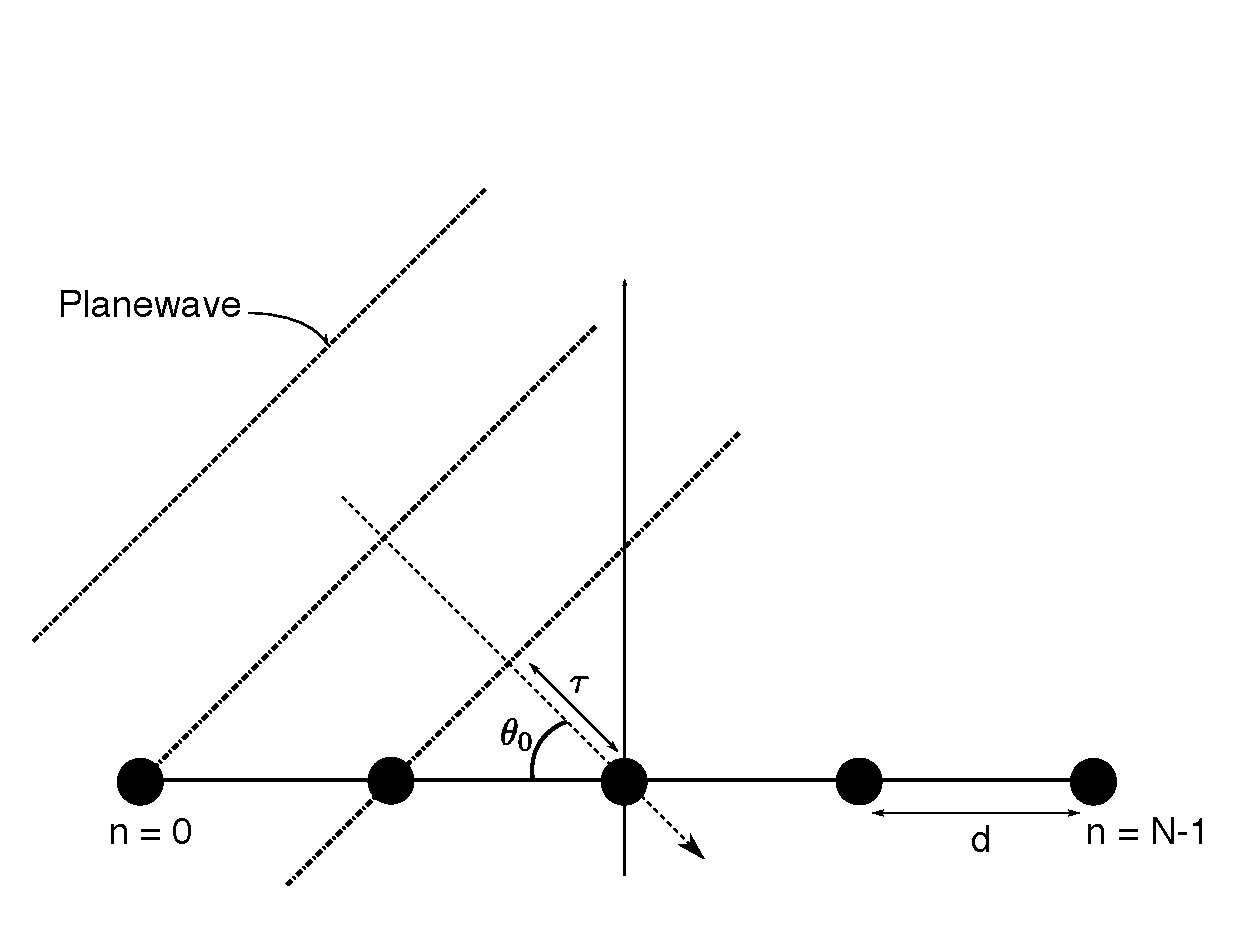
\includegraphics[width=\textwidth]{ula_planewave.pdf}
    \caption[Planewaves propagating across uniform linear array (ULA).]{Planewaves propagating across uniform linear array (ULA). The ULA has $N$ sensors (solid black circles) uniformly located at $d$ interval. The dashed arrow indicates planewave propagation direction which is expressed as angle $\theta_0$ w.r.t. the array axis. The direction along the array axis ($\theta = 0$) is called endfire and the direction perpendicular to the array axis ($\theta = \pi/2$) is called the broadside direction. The propagation time between two adjacent sensor is denoted by $\tau$.} 
 % Detailed descriptionof array geometry, broadside, endfire, bearing, axis, aperture
\label{fig:ula-geom}
\end{figure}

% The linear geometry of the ULA limits the direction resolution
% capability to elevation angles ($\theta$)
% \cite[Sec.~3.1.1]{johnson1992array}. In case of planewaves measured
% using ULAs, it is sufficient to define the propagation direction in
% terms of elevation angle. \figurename{}~\ref{fig:ula-geom} shows
% planewaves with propagation direction at an angle $\theta_0$ with
% respect to array axis. The direction along the array axis is called
% endfire ($\theta = 0$) and the direction perpendicular to the array
% axis is called broadside ($\theta = \pi/2$). Define the directional cosine
% $u = \cos(\theta)$. In the sequel, the planewave signal direction is
% denoted using directional cosine ($u$).

% Need to describe about the planewave in the figure
\figurename{}~\ref{fig:ula-geom} also shows narrowband planewaves
propagating across the ULA aperture. The dashed arrow indicates the
planewave propagation direction which is represented as angle
$\theta_0$ w.r.t. the array axis. The propagation direction along the
array axis is called endfire ($\theta = 0$) and the propagation
direction perpendicular to the array axis is called broadside
($\theta = \pi/2$). As the planewave propagates across the ULA
aperture from left to right, the planewave arrives at each sensor with
some time delay. Due to the uniform spacing of the sensors, the time
delay between adjacent sensors across the ULA is a constant
$\delay = d\cos(\theta_0)/c$ where $c$ is the speed of propagation. As
mentioned earlier, in case of narrowband planewave signals, the time
delay ($\delay$) is approximated by a phase shift
$\psi = (2\pi/\lambda)d\cos(\theta_0) = (2\pi/\lambda)d\ulook$ where
$\ulook = \cos(\theta_0)$ is the directional cosine. In the sequel, the
propagation direction of a planewave is expressed using the
directional cosine ($u$). Denoting the phase shifts at each sensor
w.r.t. a reference sensor at $p_0 = 0$ as a vector of complex
exponentials,
\begin{equation}
\label{eq:array-manifold}
  \rep(\ulook) = [1,~e^{-j{(2\pi d/\lambda)}  u_0},~ e^{-j{(2\pi d/\lambda)}2 u_0},
\ldots, e^{-j{(2\pi d/\lambda)}(N-1)  u_0}]^\text{T}.
\end{equation}
This vector of complex exponentials is referred to as the array
manifold vector \cite{vtree2002oap}. The array manifold vector
$\rep_0$ models the geometry and the spatial characteristic a ULA
observing a narrowband planewave signal with propagation direction
$\ulook$. The array manifold vector in \eqref{eq:array-manifold} is
defined such that $\norm{\rep(\ulook)}^2 = N$.

\subsection{Frequency domain snapshot model}
\label{sec:freq-snapshot}
In many cases, the beamforming operation is implemented in the frequency
domain \cite[Sec.~5.2.1]{vtree2002oap}. In the frequency domain, the ULA
measurement is expressed as a complex vector called frequency domain
snapshots. In order to generate the frequency domain snapshots, the
ULA observes the planewave signal for an interval $T$ during which the
source is assumed to be spatially stationary. The total observation
interval $T$ is divided into $L$ interval blocks of length
$\deltaT$. The following step performs an FFT on the signal observed
at each sensor for each interval block of length $\deltaT$. At each sensor, extracting the
complex coefficient from the FFT output associated to the narrowband
center frequency $f_0$ gives one snapshot vector. Let $X_n$ be the
complex coefficient associated with the $n^{th}$ sensor. The
narrowband planewave frequency domain snapshot vector is represented
as an $N \times 1$ complex vector $\x = [X_1,X_2,\ldots X_N]^T$. For a
single narrowband planewave signal propagating with directional cosine
$\ulook$, the frequency domain snapshot measured using the ULA is
modeled as $\x = a\rep_0$ where $a$ is the complex amplitude of
the planewave signal and $\rep_0 = \rep(\ulook)$ is the array manifold vector
corresponding to the planewave direction $\ulook = \cos(\theta_0)$.

% In the sequel, the frequency domain snapshot of narrowband planewave signals measured using a ULA is referred to as snapshot

\section{Planewave beamforming using a ULA}
\label{sec:beamforming} 
This section introduces beamforming with focus on narrowband planewave
signals observed using a ULA. Beamforming combines the entries of the
snapshot vector with complex weights to enhance the planewaves
arriving from a specific look direction and suppressing interfering
planewaves and noise. This operation is essentially spatial filtering
of planewave signals analogous to band pass filtering of time domain
signals where signals in a specific frequency band are allowed to pass
though while signals outside the band are
suppressed. \figurename{}~\ref{fig:beamformer} illustrates the
beamforming operation on snapshot data obtained from a ULA. The
beamformer applies a complex weight $w_n$
to each entry of the ULA snapshot vector and sums to produce a scalar
output $ y = \wt^H\datavec$,
where $\wt = [w_0, w_1, w_2\ldots w_{N-1}]^{T}$
is the beamformer weight vector. The CBF is the basic beamformer
applied to the ULA snapshot data. The CBF weights phase shifts each
snapshot entries such that planewave signals from the look direction
$\ulook$
align in time and combine constructively while signals from other
direction combine destructively and are suppressed. Hence, a CBF
steered to the look direction $\ulook = \cos(\theta_0)$
has a weight vector equal to the array manifold vector associated with
the look direction, i.e., $\wcbf = \rep_0/N$.
\begin{figure} \centering
    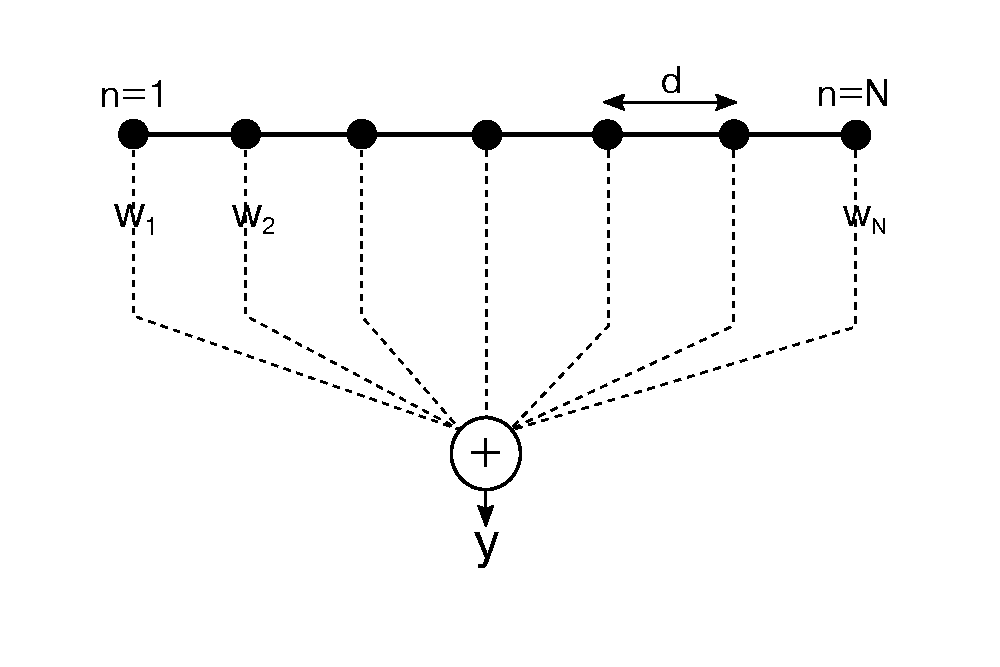
\includegraphics[width=0.7\linewidth]{beamforming}
    \caption[Beamforming operation
      scales each sensor output with complex weights.]{Beamforming operation
      scales each sensor output with complex weights ($w_n$) and
      combines them to produce scalar output $\yt$. The beamformer
      weights are analogous to FIR filter coefficients and determine
      the spatial response.}
    \label{fig:beamformer}
\end{figure}
The beamformer weights are analogous to FIR filter coefficients. As
the choice of the filter coefficients determines the frequency
response of the FIR filter, the choice of the weight vector determines
the spatial frequency response of the beamformer for a given ULA. The
beampattern defines the complex gain due to the beamformer for a unit
amplitude planewave from direction $u = \cos(\theta)$, i.e.,
\begin{equation}
  \label{eq:beampatu} 
  \beampatu = \wt^H\rep(u) = \sum_{n=0}^{N-1}w_n^*\left(\expo{-j(2\pi d /\lambda) u}\right)^n
\end{equation}
where $(\cdot)^*$ denotes conjugate and $-1 \leq u \leq 1$ is the
directional cosine. \figurename{}~\ref{fig:cbf_bp} is the log
magnitude beampattern of a CBF implemented using $N = 11$ sensor ULA
and steered to the broadside ($\ulook = 0$) look direction. The
beampattern is characterized by a mainlobe in the look direction
and multiple sidelobes outside the mainlobe. The mainlobe allows the
signal of interest to pass through while the sidelobes suppress noise
and interfering signals. For a CBF steered to the broadside using $N$
sensor ULA, the mainlobe extends from $-2/N \leq u \leq 2/N$. Outside
the mainlobe, the CBF beampattern has $N - 1$ nulls at
$\Delta u = 2/N$ interval \cite{vtree2002oap}.

\begin{figure} \centering
    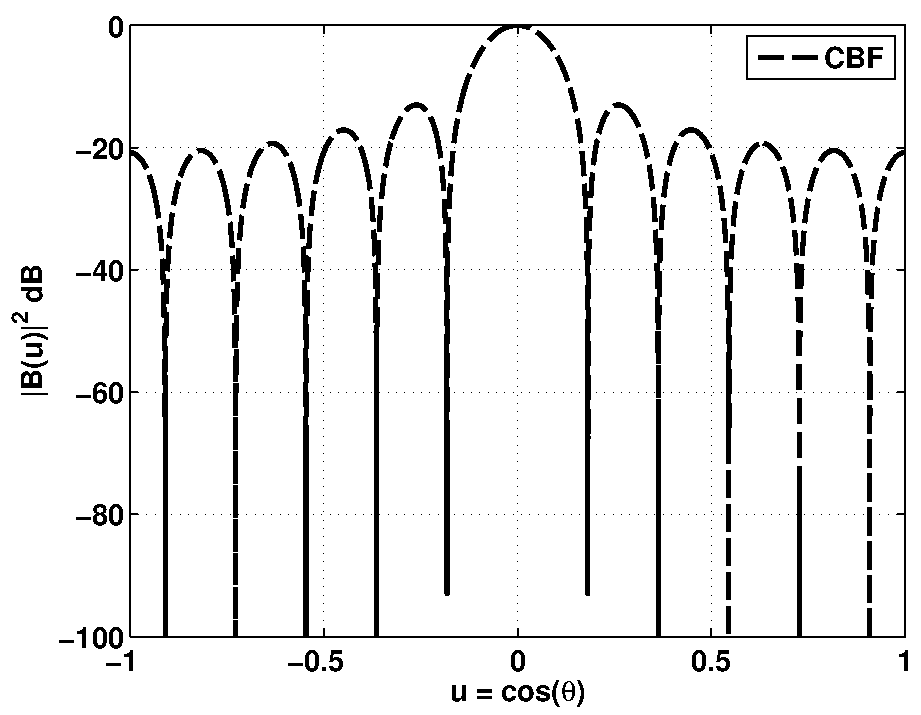
\includegraphics[width=\textwidth]{cbfbeampattern}
    \caption[Log magnitude of the CBF beampattern using an $N=11$
      sensors ULA.]{Log magnitude of the CBF beampattern using an $N=11$
      sensors ULA. The beamformer is steered towards the broadside
      ($\ulook=0$). The beampattern is characterized by a mainlobe in
      the look direction and sidelobes outside the look direction. The
      main lobe allows the signal of interest to pass through while
      the sidelobes suppress noise and interfering signals.}
    \label{fig:cbf_bp}
\end{figure}

In practice, beamformers often operate in an environment where a weak
signal of interest exists in presence of strong interfering signals
and noise. This is a common scenario in passive sonar applications
\cite{cox2002adaptive,baggeroer1999passive}. The CBF weight vector
$\wcbf$ depends only on the look direction and it produces a static
beampattern steered to the look direction. The CBF has a limited
ability to attenuate strong interferers which can leak through the
sidelobes and mask the weaker signal of interest. In such scenarios,
one approach is to design beamformers which can adapt their weights
based on measured snapshot data as discussed in \sect{}\ref{sec:abf}.

\subsection{Signal model}
\label{sec:signal-model}

This section describes the measurement signal model used in this
dissertation. The model assumes an environment consisting of multiple
narrowband planewave signals in a spatially white background noise. In
such a scenario the snapshot data is commonly modeled as
\begin{equation}
  \label{eq:array-data} \datavec = a_0\rep_0 + \sum\limits_{i=1}^D a_i\rep_i +
\noisevec,
\end{equation}
where $\rep_0$ is the desired signal array manifold vector and $a_0$
is the desired signal amplitude, $D$ is the number of interfering
signals, $a_i$ is $i^{th}$ interferer signal amplitude, $\rep_i$ is
the $i\nth$ interferer array manifold vector associated with direction
$u_i$, and $\noisevec$ is the additive white noise. This dissertation
assumes that the desired signal is absent from the snapshot
observations used to train the adaptive beamformer, i.e., $a_0 =
0$.
The interferer signal amplitude is modeled as a zero mean complex
circular Gaussian random variable, i.e.,
$a_i \sim \cnormal{0, \cov_i^2}$ and the background noise is assumed
to be spatially white with complex circular Gaussian distribution,
i.e., $\noisevec \sim \cnormal{\mathbf{0}, \cov_w^2\eye}$. Assuming
the $D$ interfering signals in \eqref{eq:array-data} are uncorrelated
and independent of noise, the interferer plus noise ensemble
covariance matrix (ECM) is
\begin{align}
  \label{eq:ecm} \Cov =& E[\datavec\datavec\herm] = \sum\limits_{i =
1}^D\cov_i^2\rep_i\rep_i\herm + \cov_w^2\eye,
\end{align}
where $\cov_i^2$ is $i^{th}$ interfering signal power and $\cov_w^2$
is the sensor level noise power. The ECM quantifies the statistical
relation between snapshot data observed at each sensor.

%\srt{Talk about interferer types and noise types sources}

\section{Adaptive beamformers}
\label{sec:abf}
Adaptive beamformers (ABF) use the knowledge of statistical properties
of the signal and noise process to compute beamformer weights which
are optimal in some statistical sense. The ABFs adjust the beampattern
to suppress the interferers and the noise. The minimum variance
distortionless response (MVDR) beamformer introduced by Capon is one
of the most commonly used ABF \cite{capon1969mvdr}. The MVDR ABF is an
optimal beamformer that minimizes the total output power but
passes planewave signals from the desired look direction
undistorted. The MVDR beamformer weight vector $\wmvdr$ solves the
constrained optimization problem
\begin{equation}
  \label{eq:mvdr-const-prob}
  \underset{\wt}\min \quad f(\wt) = 
\wt\herm\Cov\wt \quad \text{s.t.} \quad \wt\herm\replook = 1,
\end{equation}
where $\Cov$ is the interferer-plus-noise ECM and
$\replook = \rep(\ulook)$ is the array manifold vector corresponding
to the look direction $\ulook = \cos(\theta_0)$. The optimum solution
to \eqref{eq:mvdr-const-prob} gives the MVDR weight vector
\begin{equation}
  \label{eq:mvdr-wt} 
\wmvdr =
\frac{\Cov\inv\replook}{\replook\herm\Cov\inv\replook}.
\end{equation}
The weight vector $\wmvdr$ is referred to as the ensemble MVDR ABF
weight vector. \figurename{}~\ref{fig:mvdr-beampattern} is the log
magnitude beampattern of the ensemble MVDR ABF steered to the
broadside using $N = 11$ sensor ULA. A single interferer is present at
direction $\uinter = 3/N$ denoted by the vertical dotted line. The
beampattern has unity gain in the look direction and places a deep
beampattern notch in the interferer direction to suppress interferer
power and consequently minimize output power.

% When no interferer is present in the snapshot data,
% $\Cov = \noisepow\eye$. In absence of interferers, the MVDR ABF weight
% vector \eqref{eq:mvdr-wt} reduces to CBF weight vector for same look
% direction \cite{vtree2002oap}. The CBF is the optimal beamformer

\begin{figure}[!hp]
 \centering
    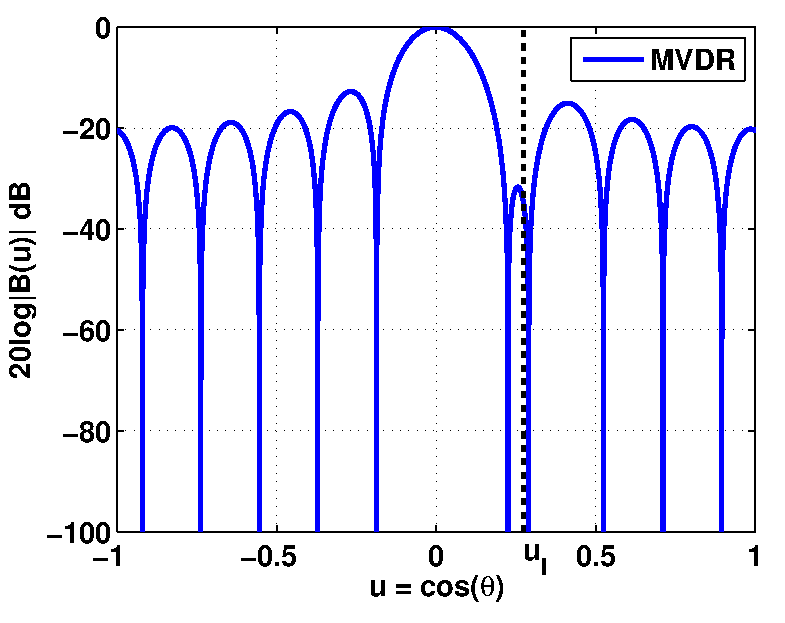
\includegraphics[width=\textwidth]{mvdr_cbf_N11_bp_plot.pdf}
    \caption[Log magnitude beampattern (solid-blue) of the ensemble MVDR ABF using $N = 11$ sensor ULA.]{Log magnitude beampattern (solid-blue) of the ensemble MVDR ABF using $N = 11$ sensor ULA. The vertical dotted line indicates a single narrowband planewave interferer present at $\uinter = 3/N$. The log magnitude beampattern for the CBF (dashed-black) using same ULA is shown for reference. The ensemble MVDR ABF places deep notch in the interferer direction compared to the CBF.} 
    \label{fig:mvdr-beampattern}
\end{figure}

% Figure showing MVDR beampattern
\subsubsection*{Notch depth}
\label{sec:notch-depth}
The magnitude squared beampattern in the interferer direction is
called the notch depth (ND), i.e.,
$\notchdepth = |\beampat{\uinter}|^2$, where $\uinter$ is the
interferer direction. The ND quantifies the interferer attenuation due
to the beamformer. The ND is defined for a particular interferer
direction $\uinter$ and it is not necessarily associated with the
local minima in the beampattern. 

In case of a single interferer with power $\interfpow$ at direction $\uinter$, the ND is
\begin{align}        
    \label{eq:ens_nd}
    \notchdepth = \frac{|\replook\herm\repint|^2/N}{\left| 1 + N \inr(1 - |\replook\herm\repint|^2) \right |^2},
\end{align}
where $\inr = \interfpow / \noisepow$ is the interference-to-noise
ratio (INR). In the single interferer case, the ND for a given
interferer depends on the number of sensors $N$ and the INR level. For
a loud interferer as $\inr \rightarrow \infty$, the
$\notchdepth \rightarrow 0$, i.e., the ensemble MVDR ABF places a null in the
interferer direction. Similar ND behavior is observed in case of multiple loud interferers \cite{vtree2002oap}.

\subsubsection*{White noise gain}
\label{sec:white-noise-gain}
White noise gain (WNG) quantifies the improvement in SNR due to
beamforming when the background noise is spatially white. Assuming
unity gain in the look direction, $\text{WNG} = 1/||\wt||^2$ where
$||\cdot||$ denotes the Euclidean norm of a vector \cite[Eq.~(2.186)]{vtree2002oap}. 
Using the Parseval's relation between the beamformer weights $\wt$ and the beampattern $\beampatu$, the WNG is expressed as
\begin{equation}
  \label{eq:wng-beampat}
   \text{WNG} = \left[\half \int\limits_{-1}^1 |\beampatu|^2 du\right]\inv.
\end{equation}
where $|\beampatu|^2$ is the magnitude squared beampattern
\cite[Eq.~(3.6)]{vtree2002oap}. Thus the WNG is inversely proportional
to the area under the magnitude squared beampattern. This relation
between the WNG and the beampattern suggests that a wider
mainlobe and higher sidelobes have negative impact on WNG. For a given
ULA, the CBF is optimal in terms of maximizing the WNG and the WNG of
the CBF equals to the number of sensors $N$. WNG is also a metric for
beamformer robustness against parameter mismatch \cite{Gilbert1955}.

\subsubsection*{Output power}
\label{sec:output-power}
The ensemble MVDR ABF output power is $\pout = E[|\wmvdr\herm\datavec|^2] = \wmvdr\herm\Cov\wmvdr$. Using the ECM definition from \eqref{eq:ecm}, the output power is
\begin{align}
  \label{eq:mvdr-ecm-pout}
  \pout =& \sum\limits_{i=1}^D\cov_i^2|\wmvdr\herm\rep_i|^2 + \norm{\wmvdr}^2  \nonumber \\
=& \sum\limits_{i=1}^D\cov_i^2\notchdepth_i + \noisepow\wng\inv \nonumber \\
=& \pinter{} + \pnoise{}
\end{align}
where $\notchdepth_i$ is the notch depth at the $i\nth$
interferer. The output power is the combination of the interferer
contribution ($\pinter$) and the white noise contribution
($\pnoise$). The ND determines the interferer contribution and the WNG
determines the white noise contribution to the output power. The
ensemble MVDR ABF adjusts the NDs and the WNG while maintaining unity
gain in the look direction, to produce the minimum output power.

\subsection{Sample matrix inversion MVDR ABF}
\label{sec:smi-mvdr}
The ensemble MVDR ABF uses the knowledge of the ECM to compute the
weight vector in \eqref{eq:mvdr-wt}. In practical situations the ECM
is unknown and so it has to be approximated from the observed snapshot
data. The ECM is commonly estimated by computing the sample covariance
matrix (SCM) from a finite number of snapshots as
\[ 
\sampCov = \frac{1}{L}\sum\limits_{l=1}^{L}\datavec_l\datavec_l\herm
\]
where $L$ is the number of snapshots and $\datavec_l$ is the
$l^{th}$ snapshot vector defined in \eqref{eq:array-data}. The SCM is
the maximum likelihood estimate of the ECM
\cite[Sec. 7.2.1]{vtree2002oap}. In the practical implementation the SCM replaces the ECM in \eqref{eq:mvdr-wt} to compute the ABF weight vector. Computing
the SCM based MVDR ABF weight vector involves inverting the SCM and
the resulting ABF is referred to as the sample matrix inversion (SMI)
MVDR ABF. The SMI MVDR ABF weight vector is
\begin{equation*}
  \label{eq:smi-wt}
  \wsmi = \frac{\sampCov\inv\replook}{\replook\herm\sampCov\inv\replook} .
\end{equation*}
Here again $\replook$ is the look direction array manifold vector and it is assumed to be known. 

The SMI MVDR ABF relies on availability of large number of snapshot
(${L \gg N}$) so that the SCM gives an accurate estimate of the ECM
\cite{boroson1980sample}. Reed et al.\ show that at least two
snapshots per sensor, i.e., $L \geq 2N$ is required to ensure the
output SINR loss due to the use of SCM instead of the ECM is less than
$3$ dB \cite{reed1974rapid}. In many beamforming scenarios, such as
passive sonar, physical non-stationarities in the environment or
source locations preclude averaging large numbers of snapshots to form
the SCM. Cox and Baggeroer show that in a moving source scenario, the
usable number of snapshots available for SCM averaging is inversely
proportional to array aperture and source velocity
\cite{baggeroer1999passive, cox2000mrabf}. The use of long arrays and
the presence of fast moving sources severely limit the available
number of snapshots. In many passive sonar applications it is common
to have only limited snapshots ($L \approx N$) or even insufficient
snapshots ($L < N$) available and even two snapshots per sensor
($L = 2N$) is considered a snapshot rich case.

When the number of snapshots are limited ($L \approx N$) the SCM is
ill-conditioned and the SCM inversion is numerically
unstable. Inadequate estimation of the SCM results in high sidelobes
and distorted mainlobe in the beampattern and subsequent loss of the
NDs and WNG \cite{Carlson1988scm, richmond2000mvdr}. Moreover, in a
snapshot deficient case $L < N$, the SCM is rank deficient and the SCM
inversion is not possible.

%  In radar and mobile communication scenario, ABFs operate are
% operating in more and more dynamic environments consisting of fast
% moving targets or interferers or co-channel interferer sources
% \cite{riba1997comm}. Operating in dynamic environments requires fast
% adaptive processing. The ABF weights have to be updated fast enough to
% keep up with changing scenario. Unable to do so results in degraded
% performance. This requirement constrains the usable number of
% snapshots before beamformer weights need to be updated and it results
% in $N \approx \mathcal{O}(L)$.

\subsubsection{Diagonal loading}
\label{sec:diagonal-loading}
One solution applies diagonal loading to the SCM to address the
ill-conditioned or rank deficient condition. A diagonal loaded (DL)
SCM is $\sampCov_\dl = \sampCov + \dl\eye{}$, where $\dl > 0$ is the
DL factor \cite{Carlson1988scm}. Diagonal loading ensures that the
modified SCM $\sampCov_{\dl}$ is full rank and invertible to compute
the beamformer weights. Substituting the ECM with the DL SCM
$\sampCov_{\dl}$ in \eqref{eq:mvdr-wt} computes the DL MVDR ABF
weights,
\begin{equation*} 
    \label{eq:dlmvdr}
{\bf \wts}_{\dl} = \frac{\sampCov_{\dl}\inv \replook}{\left(\replook\herm
\sampCov_{\dl}\inv \replook \right)}.
\end{equation*}
Applying diagonal loading essentially adds white noise power to the SCM. In
effect, the DL MVDR ABF weight vector is designed for a higher level
white noise power than is actually present in the observed
snapshot. As a result the DL MVDR ABF improves white noise suppression. Also, asymptotically as the DL factor increases such that
$\dl \rightarrow \infty$,
the DL SCM $\sampCov_\dl \approx \dl\eye$
and the DL MVDR ABF approaches the CBF \cite{vtree2002oap}.

In addition to enabling implementation of the SMI ABFs in a snapshot
deficient scenario, diagonal loading also enables better WNG and
improves robustness against parameter mismatch \cite{vtree2002oap,
  mestre2005diagonal}. However, implementing the DL MVDR ABF requires
choosing the DL factor. Appropriate choice of the DL factor requires
knowledge of the interference and noise power levels which are unknown
in practice. Several approaches have been proposed for choosing the
appropriate DL factor. Mestre and Lagunas introduced a random matrix
theory based estimator for the optimal DL factor with focus on
snapshot limited scenarios \cite{mestre2005diagonal}. The authors
derive an expression relating the asymptotic output SINR to the DL
factor $\dl$ and the ratio of snapshots per sensor. The optimal DL
factor is a solution that maximizes the output SINR. However, the
procedure to search for the optimal DL factor has a significantly
higher computational complexity compared to other procedures to
estimate the DL factor.

% =======================================================================

\subsection{Dominant mode rejection ABF}
\label{sec:dmr-abf}
Abraham and Owsley introduced the dominant mode rejection (DMR) ABF
\cite{abraham1990beamforming}. The DMR ABF uses a structured estimate
of the SCM to compute the ABF weight vector. The DMR ABF weight vector
has the same form as the SMI MVDR weight vector \eqref{eq:smi-wt} but
the DMR algorithm replaces the SCM with a structured estimate derived
from the eigendecomposition of the SCM. The DMR ABF uses
eigendecomposition to partition the SCM into a subspace containing the
dominant eigenvectors and the orthogonal noise subspace. The dominant
eigenvectors correspond to the interferers that the ABF has to
suppress. In the structured estimate, the noise eigenvalues are
replaced their average value while keeping the dominant eigenvalues intact \cite{vtree2002oap}.
\clearpage
The DMR algorithm assumes the snapshot data includes $D$ planewave
interferers plus colored noise, and white noise. The
eigendecomposition of the SCM is
\[
\sampCov = \sum\limits_{n = 1}^{N}\sampeval_n\sampevec_n\sampevec_n\herm,
\]
where $\sampeval_1 \geq \sampeval_2 \geq \ldots \geq \sampeval_n$ are
the sample eigenvalues and $\sampevec_n$s are the corresponding sample
eigenvectors. The eigenvectors corresponding to the $D$ largest
eigenvalues define the dominant interferer subspace. The DMR algorithm
forms the structured approximation to the SCM using the dominant
subspace plus the noise subspace with equal power for each noise
eigenvector,
\begin{equation}
  \label{eq:dmr-scm}
\sampCovdmr = \sum\limits_{n = 1}^{D} \sampeval_n\sampevec_n\sampevec_n\herm + \sum\limits_{n = D + 1}^{N} \noisepow\sampevec_n\sampevec_n\herm,
\end{equation}
where $\sampCovdmr$ is the estimated DMR SCM and $\noisepow$ is the
estimated noise power $ \noisepow = (\sum\limits_{n = D + 1}^{N}\sampeval_n)/(N- D).$
The DMR SCM is effectively approximating the measured noise field with
a white noise field of power $\noisepow$.  The DMR ABF weight vector is simply
the SMI MVDR weight vector \eqref{eq:smi-wt} with the SCM replaced by
the DMR SCM $\sampCovdmr$,
\[
\wdmr = (\sampCovdmr\inv\replook)/(\replook\herm\sampCovdmr\inv\replook).
\]
The DMR SCM in \eqref{eq:dmr-scm} assumes that the dominant subspace dimension $D$ is known. In practice the number of planewave signals present in the measurement is usually unknown. Hence the dominant space dimension needs to be estimated before the DMR SCM can be computed.

% Also, using the estimated
% noise power ($\noisepow$) as the eigenvalue for the noise subspace
% eigenvectors removes the small eigenvalues of the SCM that cause
% problems with inverting the SCM.

\section{Array polynomials}
\label{sec:array-poly}
The beampattern of a planewave beamformer using a ULA can be
represented as a complex polynomial
\cite{Schelkunoff1943array, Steinberg1976}. Letting $d = \lambda/2$ and
$z = e^{j\pi u}$ in the definition of beampattern \eqref{eq:beampatu} yields the array polynomial
\begin{equation}
  \label{eq:beampat-poly}
  \beampolyz{} = \sum\limits_{n=0}^{N-1} w^*_n z^{-n} = \ztrans(\wt\herm).
\end{equation}
$\beampolyz{}$ is an $N-1$ degree polynomial in complex variable $z$
and the conjugated complex beamformer weights ($w^*_n$) are the
coefficients. The array polynomial maps the directional cosine ($u$)
variable into a complex plane variable ($z$). The phase of the complex
variable $z$ is related to the directional cosine $u$ as
$\operatorname{arg}(z) = \pi u$. Also the definition in
\eqref{eq:beampat-poly} is identical to the $z$-transform of the
conjugate beamformer weights \cite[Chap.~3]{Oppenheim1989}. The array
polynomial of a beamformer is analogous to the system function of a DT
FIR filter \cite{Oppenheim1989}. Evaluating the array polynomial
\eqref{eq:beampat-poly} on the unit circle
$\lbrace z \in \mathbb{C}, |z| = 1\rbrace$ yields the beampattern
\eqref{eq:beampatu}. Continuing the analogy with DT FIR filters, the
beamformer array polynomials also have pole-zero representation on the
complex plane. For a beamformer for an $N$ sensor ULA, the array
polynomial has $N - 1$ zeros and the corresponding $N - 1$ poles at
the origin. Thus the array polynomial zeros on the unit circle create
nulls in the beampattern. The array polynomial defined in
\eqref{eq:beampat-poly} is associated with the beamformer implemented
using a ULA. In the sequel the array polynomial is referred to as the
beamformer polynomial. This thesis uses the ABF polynomial
representation to analyze and synthesize beampatterns by manipulating
the polynomial zeros.

\subsection{CBF polynomial}
\label{sec:cbf-polynomial}

A CBF steered to the broadside ($\ulook = 0$) has weight vector
$\wcbf = \mathbf{1}/N$. The $z$-transform of $\wcbf$ gives the CBF
polynomial
\begin{align}
  \label{eq:cbf-poly}
  \cbfpoly = \frac{1}{N}\sum\limits_{n=0}^{N-1}z^{-n} 
  = \frac{1}{N}\left[\frac{z^N - 1}{z^{N-1}(z - 1)}\right].
\end{align}
\eqn{}\eqref{eq:cbf-poly} shows that the CBF polynomial zeros
$\ensz_n$ are the $N\nth$ roots of unity except for the one at
$z = 1$, i.e., $\ensz_n = \expo{2\pi n/N}$ for $n = 1,\ldots, N-1$.
\figurename{}~\ref{fig:unit-circle} shows array polynomial zeros for a
CBF using an $N = 11$ sensor ULA. All the CBF polynomial zeros are
confined onto the unit circle and these zeros produce nulls in the CBF
beampattern shown in \figurename{}~\ref{fig:cbf_bp}. The unit circle
point $z_0 = 1$ corresponds to the broadside look direction and the
two adjacent zeros at $z = \expo{\pm j2\pi/N}$ are associated with the
first nulls of the CBF beampattern in \figurename{}~\ref{fig:cbf_bp}.

\begin{figure}[!hp]
 \centering
    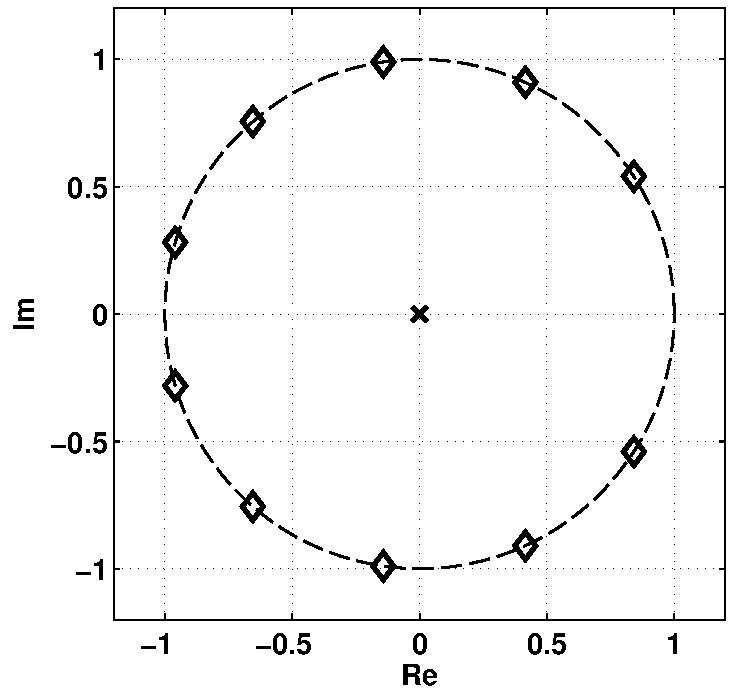
\includegraphics[width=0.75\textwidth]{cbf_pzplot_N11_INR0.pdf}
    \caption[CBF polynomial zeros for beamforming using an $N = 11$
      sensor ULA.]{CBF polynomial zeros for beamforming using an $N = 11$
      sensor ULA. All the CBF polynomial zeros fall on the unit circle. These zeros produce nulls in the CBF beampattern.}
    \label{fig:unit-circle}
\end{figure}

%%% Local Variables: 
%%% mode: latex
%%% TeX-master: "main"
%%% End:  
\chapter{MVDR ABF polynomial zeros }
\label{ch:mvdr-polyn-zeros}
The $z$ transform of the conjugated weights of the ABF produce the ABF
array polynomial. Evaluating the ABF polynomial on the unit circle
yields the beampattern. The ABF polynomial zeros on the unit circle
are associated with the ABF beampattern nulls. The ABFs use the
knowledge of the operating environment to adjust the beampattern to
achieve optimal output. As the ABFs adjust the beampattern, the
associated ABF polynomial zeros also change location on the complex
plane. This chapter focuses on the ensemble MVDR ABF polynomial and
its zeros. The first section presents the ensemble MVDR ABF polynomial
and the properties of its zeros. The second section develops a model
for the location of the ensemble MVDR polynomial zeros as a function
of interferer power. The final section discusses the behavior of the
SMI MVDR ABF polynomial zeros.

\section{Ensemble MVDR ABF polynomial}
\label{sec:mvdr-polynomial}
The ensemble MVDR ABF polynomial is
$\mvdrpoly{z} = \ztrans(\wmvdr\herm)$ where $\ztrans(\cdot)$ denotes
the $z$ transform operation and $\wmvdr$ is the ensemble MVDR ABF
weight vector. Factoring the polynomial in terms of the zeros,
\[
\mvdrpoly{z}  =  \Gamma \prod\limits_{n=1}^{N-1}(1 - \ensz_n z\inv),
\]
where $\Gamma$ is a scaling term to ensure unity gain in the look
direction ($\ulook$), i.e., $\mvdrpoly{\expo{j\pi\ulook}} = 1$ and
$\ensz_n$ is the $n^{th}$ zero. The ensemble MVDR ABF polynomial zeros
will be referred to as ensemble zeros in the
sequel. \figurename{}~\ref{fig:mvdr-plots} shows the ensemble zeros
and log magnitude of the beampattern for an example case of the
ensemble MVDR ABF using $N = 11$ sensor ULA. A single interferer is
present at $\uinter = 3/N$ and the interferer-to-noise power ratio
(INR) is 10 dB. The dashed radial line in
\figurename{}~\ref{fig:mvdr-pzplot} indicates the phase angle
$\pi\uinter$ corresponding to the interferer direction
$\uinter$. Denote the unit circle point corresponding to the
interferer direction as $\interz = \expo{j\pi\uinter}$. In the complex
plane, all $10$ ensemble zeros fall on the unit circle. These unit
circle zeros produce the beampattern nulls seen in the log magnitude
beampattern plot \figurename{}~\ref{fig:cbf-mvdr-bpplot}. The vertical
dotted line in the beampattern plot indicates the interferer direction
($\uinter$).

\begin{figure}[!hp]
  \centering
  \subfloat[]{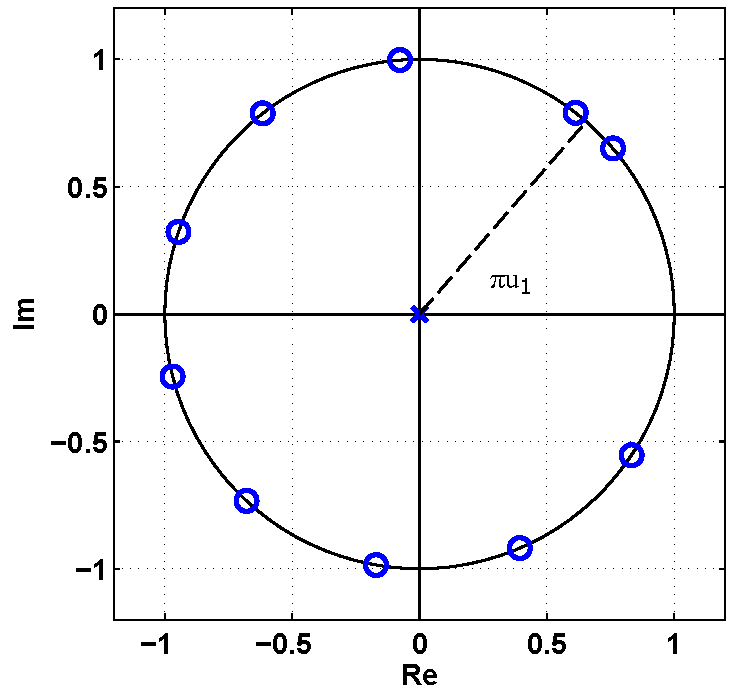
\includegraphics[width=3.5in]{mvdr_cbf_pzplot_N11_INR0}
    \label{fig:mvdr-pzplot}} \hfill
  \subfloat[]{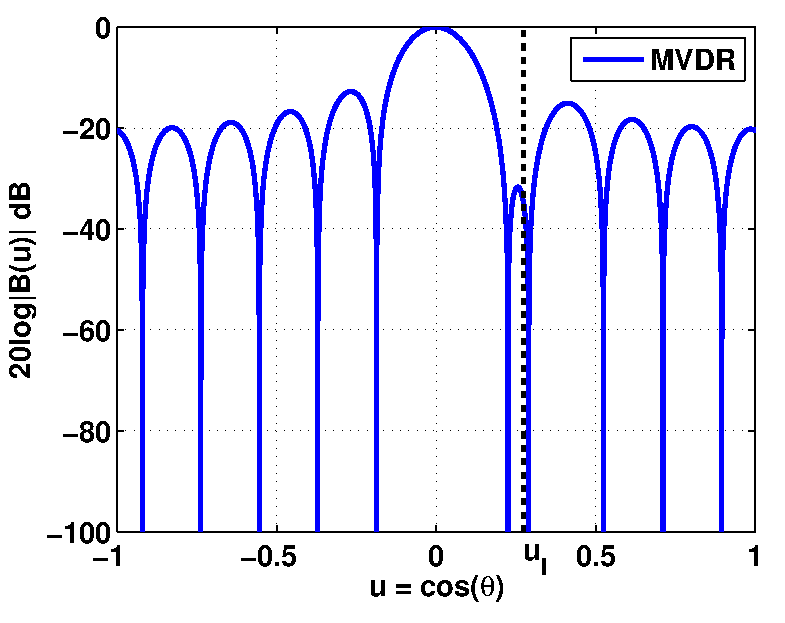
\includegraphics[width=3.5in]{mvdr_cbf_N11_bp_plot}
  \label{fig:cbf-mvdr-bpplot}}
\caption[Ensemble MVDR ABF polynomial zero locations]{Ensemble MVDR ABF \protect\subref{fig:mvdr-pzplot} polynomial
  zero locations and \protect\subref{fig:cbf-mvdr-bpplot} log
  magnitude of beampattern for an example case using $N = 11$ sensor
  ULA. A single interferer is present at $\uinter = 3/N$ indicated by
  vertical dashed line in \protect\subref{fig:cbf-mvdr-bpplot}. In
  \protect\subref{fig:mvdr-pzplot} the dashed radial line at indicates
  the phase angle $\pi\uinter$. The ensemble zeros are constrained on
  the unit circle and produce nulls in the beampattern.}
  \label{fig:mvdr-plots}
\end{figure}

Expanding to a multiple planewave interferer case, numerical
experiments found that the ensemble zeros are still constrained to the
unit circle. 50000 independent ensemble MVDR weight vectors were
generated for an $N = 11$ sensor ULA. In each scenario there were a
random number of interferers with counts ranging from
$1~\text{to}~10$, at random locations between $-1\leq u \leq 1$ and
INR level randomly set between 10 to 40 dB. The ensemble zeros in all
50000 scenarios were on the unit circle. Repeating this experiment
with a $N = 41$ sensor ULA found the same result. In fact the MVDR
ensemble zeros are always constrained on the unit circle for planewave
beamforming using ULAs. Steinhardt and Guerci found similar behavior
of the ensemble zeros, but the result does not appear to be widely
known \cite{steinhardt2004stap}. Steinhardt and Guerci present a proof
for the unit circle constraint on MVDR ensemble zeros which is
restated in Appendix~\ref{sec:apdx-mvdr-zeros}.

% Remainder of the chapter considers the single interferer case?

\section{Ensemble zero location on the unit circle}
\label{sec:mvdr-interf-suppr}
The unit circle constrained ensemble zeros create $N-1$ nulls in the
beampattern. But the ensemble MVDR ABF does not necessarily place the
nulls in the interferer directions. Numerical experiments show that
the ensemble MVDR ABF places a null in the vicinity of the interferer
direction to produce a deep notch at the interferer
direction. \figurename{}~\ref{fig:mvdr-notch-zoom} shows a zoomed
section of the ensemble MVDR ABF beampatterns in the neighborhood of
the interferer direction ($\uinter$). The vertical solid line
indicates interferer direction. The three beampatterns correspond to
the ensemble MVDR ABFs implemented for INR levels of $5$ dB (solid),
$10$ dB (dashed) and $15$ dB (dash-dot). The ensemble MVDR ABF adapts
the notch depth (ND) at the interferer direction according to the INR
level as discussed in \sect{}\ref{sec:notch-depth}. As the INR
increases, the beampattern null shifts towards the interferer
direction yielding a deeper notch. As INR decreases, the beampattern
null shifts away from the interferer direction yielding a shallower
notch. The change in beampattern null direction is replicated as
change in the location of the corresponding ensemble zero on the unit
circle.

\begin{figure}[!hp]
  \centering
  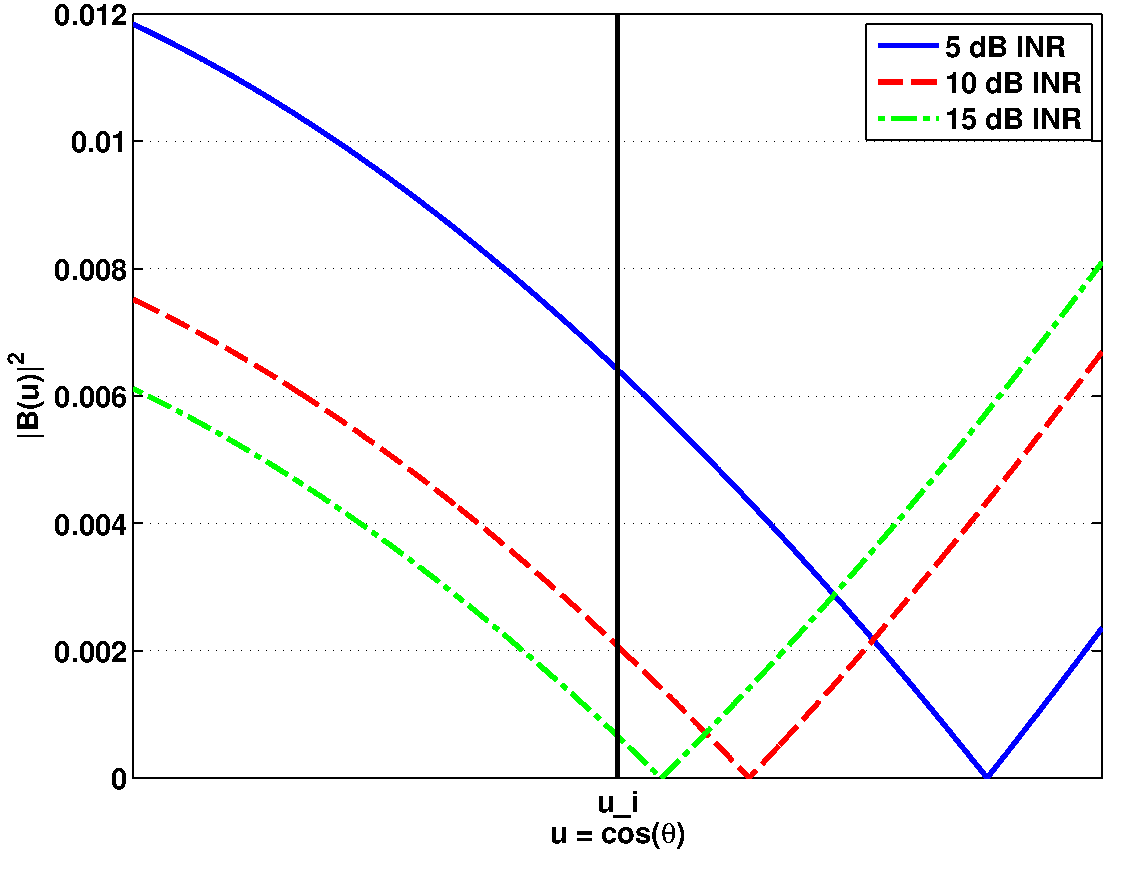
\includegraphics[width=\textwidth]{single_interf_mvdr_bp_zoom.pdf}
  \caption[Zoomed in section of the ensemble MVDR ABF
    beampatterns.]{Zoomed in section of the ensemble MVDR ABF
    beampatterns. The ABF is implemented using $N = 11$ sensor ULA and
    a single interferer is present at $\uinter$. The solid vertical
    line denotes the interferer direction. The three beampatterns
    correspond to ensemble MVDR ABF implemented for the cases of INR =
    $5$ dB, $10$ dB and $15$ dB. The ensemble MVDR ABF adjusts the
    notch depth at the interferer direction by shifting the
    beampattern null closer to the interferer direction as the
    interferer power increases.}
  \label{fig:mvdr-notch-zoom}
\end{figure}

The ensemble zeros shift along the unit circle as the ensemble MVDR
ABF adjusts the beampattern to the interferer and the noise. Since the
ensemble zeros are constrained on the unit circle it is sufficient to
observe the phase angle of the ensemble zeros to examine their
location on the complex
plane. \figurename{}~\ref{fig:mvdr-zeros-phase} shows the phase angle
of the ensemble zeros as the INR changes from $-40$ dB to $40$ dB for
an example case of the ensemble MVDR ABF using an $N = 11$ sensor ULA
and steered towards broadside ($\ulook = 0$). A single interferer is
present at $\uinter = 3/N$. The solid curves denote the phase angle of
each of the $10$ ensemble zeros over the range of INR values. The
dashed horizontal line denotes the phase angle of the interferer point
$\interz = \expo{j\omega_I}$. The phase angle corresponding to the
look direction is $\omega_0 = 0$. The phase angles are expressed as
fraction of $\pi$ for convenience. For the following discussion,
denote the ensemble zero producing the black curve as $\ensz_1$ and
the ensemble zero producing to the magenta curve as $\ensz_2$. The
ensemble zeros $\ensz_1$ and $\ensz_2$ are the two zeros closest to
the interferer point.

As discussed in \sect{}\ref{sec:mvdr} the ensemble MVDR ABF simplifies
to the CBF for the case of zero interferer power. In
\figurename{}~\ref{fig:mvdr-zeros-phase}, for INR levels $< -20$ dB,
the solid curves are uniformly spaced in phase angle except at the
look direction phase angle. This uniform phase angle spacing indicates
that the ensemble zeros are approximately in the CBF polynomial zero
locations. As the INR increases the black curve and the magenta curve
shift towards the horizontal dashed line. This implies that the two
zeros $\ensz_1$ and $\ensz_2$ shift closer to the interferer point
($\interz$). Approximately beyond INR $> 10$ dB INR only the black
curve continues to move closer to the horizontal dashed line while the
magenta curve stop shifting. This implies that only the closest zero
($\ensz_1$) continues to move towards the interferer point for higher
INR values. Asymptotically as INR grows large, the ensemble zero
$\ensz_1$ approaches the interferer point $\interz$ and the ensemble
MVDR beamformer asymptotically places a null in the interferer
direction \cite{vtree2002oap}. Over the range of INR values examined
in \figurename{}~\ref{fig:mvdr-zeros-phase}, only two ensemble MVDR
polynomial zeros closest to the interferer change location with change
in INR level and the rest are approximately in the CBF polynomial zero
locations. In fact, at higher INR levels, only the closest ensemble
zero $\ensz_1$ is sensitive to the INR level. This suggests that for
strong interferers, the notch depth adaptation is dominated by the
single null corresponding to the ensemble zero
$\ensz_1$. Additionally, the continuous solid curves indicate that
each ensemble zero for a particular INR level has an associated CBF
polynomial zero location. The following section develops a model that
characterizes the phase angle of $\ensz_1$ as a function of the INR.

% the change in the closest zero $\ensz_1$ in terms of the perturbation
% of $\ensz_1$ from the interferer direction on the unit circle.

\begin{figure}[!hp]
  \centering
  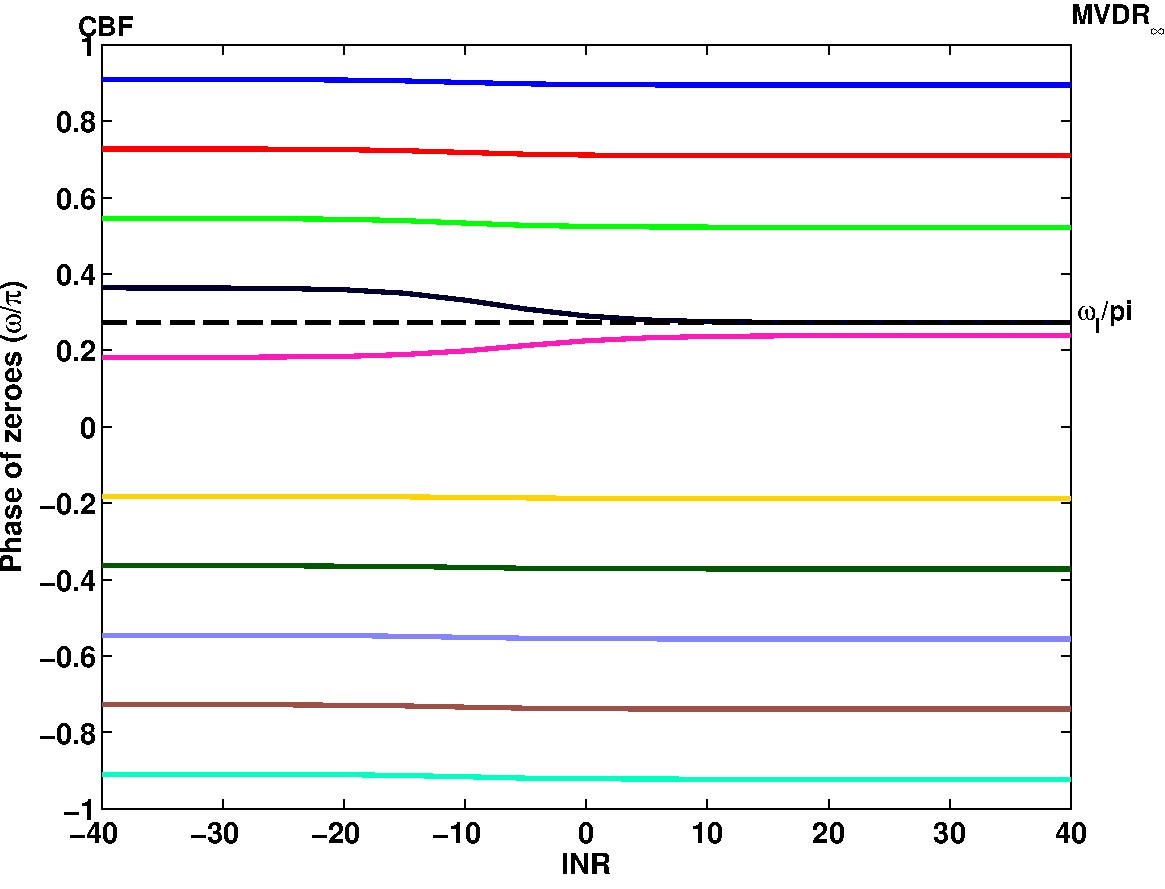
\includegraphics[width=6in]{mvdr_zeros_phase}
  \caption[Phase angle of the ensemble MVDR ABF polynomial
  zeros]{Phase angle of the ensemble MVDR ABF polynomial zeros for a
    range of INR values. The ABF is implemented using an $N = 11$
    sensor ULA and a single interferer is present at $\uinter = 3/N$.
    The phase angle of the interferer direction is denoted by the
    horizontal dashed line. Only the ensemble zeros corresponding to
    the black and the magenta curve are sensitive to INR.}
  \label{fig:mvdr-zeros-phase}
\end{figure}

% =======================================================================
\section{Ensemble zero phase angle perturbation}
\label{sec:perturbation-model}
This section develops an approximate model for the location of the
ensemble zeros ($\ensz_n$) based on the observations in
\figurename{}~\ref{fig:mvdr-zeros-phase}. The model makes following
assumptions:
\begin{itemize}
\item A single strong interferer is present in the direction
  $\uinter$. The model focuses in the region where INR $\geq 10$ dB in \figurename{}~\ref{fig:mvdr-zeros-phase}.
\item Only the location of the ensemble zero closest to the interferer
  direction is sensitive to the INR level. The closest zero is denoted
  by $\ensz_1$. This model ignores the dependence of the second
  closest zero $\ensz_2$ on the INR, demonstrated by magenta curve in
  \figurename{}~\ref{fig:mvdr-zeros-phase}.
\item The remaining $N - 2$ ensemble zeros are approximated to be in
  the CBF polynomial zero positions. For a given ULA size, the CBF
  polynomial zero locations are known \cite{vtree2002oap}.
\end{itemize}

\begin{figure}[!hp]
  \centering
  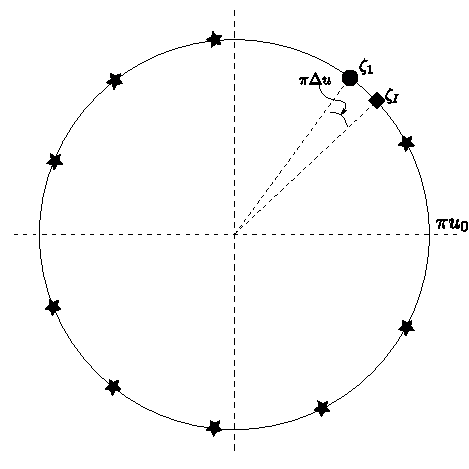
\includegraphics[width=6in]{unit_arc_zeros_pertb.pdf}
  \caption[Approximate model for ensemble zero locations]{Approximate model for
    ensemble zero locations. The diamond marker denotes the interferer
    point ($\interz$) on the unit circle. The circle marker denotes
    the ensemble zero closest to the interferer and its location is
    expressed as phase angle perturbation of $\deltau$ from the
    interferer point. The phase angle perturbation $\deltau$ depends
    on the INR level. The star markers denote the CBF polynomial zeros
    which approximate the location of the remaining $N - 2$ ensemble
    zeros. The CBF polynomial zero locations are independent of the
    INR level.}
  \label{fig:perturb-model}
\end{figure}

\figurename{}~\ref{fig:perturb-model} shows the ensemble zero
configuration based on the assumptions stated above for the case of an
ensemble MVDR ABF implemented using a $N = 11$ sensor ULA. The diamond
marker denotes the interferer point ($\interz$) and the circle marker
denotes the ensemble zero $\ensz_1$. The phase angle of $\ensz_1$ is
defined as some perturbation from the interferer point phase angle,
i.e., $\ensz_1 = \expo{j\pi u_1} =\expo{j\pi(\uinter + \deltau)}$. The
phase angle perturbation $\deltau$ depends on the INR level. The star
markers denote the remaining $10$ ensemble zeros which are
approximated to be in the CBF zero locations which are independent of
the INR level. Based on the ensemble zero configuration in
\figurename{}~\ref{fig:perturb-model}, the ensemble MVDR ABF
polynomial is,
\begin{align*} 
  \mvdrpoly{z} &\approx \left(\prod\limits_{n=2}^{N-1}\frac{1 - \cbfz_n z\inv}{1 - \cbfz_n}\right) \left(\frac{1 - \ensz_1 z\inv}{1 - \ensz_1}\right).
\end{align*}
where $\cbfz_n$ denote the $N-2$ CBF zeros. Expressing $\ensz_1$ as a
complex exponential, the MVDR polynomial becomes a bivariate function
of the complex variable $z$ and the perturbation parameter $\deltau$,
\begin{align}
  \label{eq:mvdr-approx-poly}
  \mvdrpoly{z, \deltau}  &\approx \left(\prod\limits_{n=2}^{N-1}\frac{1 - \cbfz_n z\inv}{1 - \cbfz_n}\right) \left(\frac{1 - \expo{j\pi(\uinter + \deltau)}z\inv}{1 - \expo{j\pi(\uinter + \deltau)}}\right) \nonumber \\
                         &\approx \cbfNtwozeropoly(z)\funczero{z}.
\end{align}
$ \mvdrpoly{z, \deltau}$ is the approximate ensemble MVDR ABF
polynomial.  Using the approximate MVDR ABF polynomial, the magnitude
squared beampattern is
\begin{align} 
  \label{eq:bp-poly-perturb}
  |\beampat{u, \deltau}|^2  &= |\mvdrpoly{\expo{j\pi u}, \deltau}|^2 \nonumber\\
  &= |\cbfNtwozeropoly(u)|^2 \
  |\funczero{\expo{j\pi u}} |^2 \nonumber\\
  &= |\cbfNtwozeropoly(u)|^2 \left( \frac{\sin(\pi(u - \uinter -
      \deltau)/2)}{\sin(\pi(\uinter + \deltau)/2} \right)^2.
\end{align}

Using the beampattern defined in \eqref{eq:bp-poly-perturb}, the interferer contribution to output power is
\begin{align} 
  \label{eq:approx-inter-pout}
  \interfout(\deltau) &= \interfpow|\beampat{\uinter, \deltau}|^2 \nonumber \\
&= \interfpow|\mvdrpoly{\expo{j\pi\uinter}, \deltau}|^2 \nonumber \\
&= \interfpow|\cbfNtwozeropoly(\uinter)|^2 |\funczero{\expo{j\pi \uinter}} |^2.
\end{align}
Similarly, using the definition of WNG in \eqref{eq:wng-beampat} the white noise contribution to output power is
\begin{align} 
\label{eq:approx-wn-pout}
  \noiseout(\deltau) &= \noisepow\left(\half\int_{-1}^{1}|\beampat{u, \deltau}|^2\, du\right) \nonumber \\
&= \noisepow\left(\half\int_{-1}^{1}|\mvdrpoly{\expo{j\pi u}, \deltau}|^2\, du\right) \nonumber \\
&= \noisepow\left(\half\int_{-1}^{1} |\cbfNtwozeropoly(u)|^2 |\funczero{\expo{j\pi \uinter}} |^2\, du\right).
\end{align}
As previously seen in \sect{}\ref{sec:mvdr}, when the observed
snapshot contains a single planewave interferer in a white noise, the
ensemble MVDR ABF output power is the sum of the contributions from
the interferer and the white noise. Hence, the total output power is
the sum of \eqref{eq:approx-inter-pout} and \eqref{eq:approx-wn-pout}
expressed as a function of $\deltau$,
\begin{equation}
  \label{eq:pout-deltau}
  \mvdroutput(\deltau) = \interfout(\deltau) + \noiseout(\deltau).  
\end{equation}

The ensemble MVDR ABF is the optimal ABF that minimizes the output
power for a given interferer and noise scenario
(\sect{}\ref{sec:mvdr}). This implies that for a given INR level the
optimal value of $\deltau$ in \eqref{eq:pout-deltau} should also
minimize the output power. Assuming unity gain in the look direction
and no parameter mismatch, the minimum output power is achieved when
the sum of two terms in \eqref{eq:pout-deltau} is also minimum. Taking
derivative of \eqref{eq:pout-deltau} w.r.t $\deltau$ and equating to
zero,
\begin{align}
  \label{eq:derivative-equation}
  \frac{d\,\mvdroutput(\deltau)}{d\deltau} &= 0 \nonumber \\
 \frac{d\,\interfout(\deltau)}{d\deltau} &= -\frac{d\,\noiseout(\deltau)}{d\deltau}.
\end{align}
Substituting \eqref{eq:approx-inter-pout} and \eqref{eq:approx-wn-pout} in \eqref{eq:derivative-equation} and evaluating the derivatives gives
\begin{align}
\label{eq:deltau-model}
-\interfpow \pi\deltau C &=  \noisepow (-A + \pi\deltau B),
\nonumber \\
% -\frac{\interfpow}{\noisepow} \pi \deltau C &= -A + \pi\deltau B
% \nonumber \\
\intertext{ and solving the equation yields}
\deltau &= \frac{A/\pi}{B + \inr \, C}
\end{align}
where $A$, $B$ and $C$ are constants derived in
Appendix~\ref{app:apdx-derivation} and $\inr = \interfpow/\noisepow$
is the INR. Eq.~\eqref{eq:deltau-model} is the optimal phase angle
perturbation expressed as function of the INR. The functional form of
\eqref{eq:deltau-model} is similar to a first-order lowpass filter
transfer function with INR ($\inr$) as the variable
\cite{Oppenheim1989}. As the INR $\inr\rightarrow \infty$ the phase
angle perturbation $\deltau \rightarrow 0$. Consequently the ensemble
zero $\ensz_1$ falls exactly over $\interz$ and the ensemble MVDR ABF
places a null in the interferer direction. As the INR ($\inr$)
decreases, the phase angle perturbation ($\deltau$) increases and the
ensemble zero $\ensz_1$ moves away from $\interz$. This behavior of
the ensemble zero $\ensz_1$ described by \eqref{eq:deltau-model} is
consistent with the observations in
\figurename{}~\ref{fig:mvdr-notch-zoom}.

For a particular INR level \eqref{eq:deltau-model} gives the optimal
choice of $\deltau$. Using the optimal $\deltau$ in
\eqref{eq:pout-deltau} gives the optimal output power. The optimal
$\deltau$ balances the improvement in interferer suppression with
degradation in white noise suppression as suggested in
\eqref{eq:derivative-equation}. Thus ensemble MVDR ABF can be seen as
placing a null in the vicinity of the interferer direction to create
an optimal combination of the interferer contribution ($\interfout$)
and the white noise contribution ($\noiseout$) to produce the minimum
output power.

%% Added later SRT ##################
% Any given interferer direction $\uinter$ always falls within $1/N$
% interval of the closest CBF null location for the given ULA
% size. Hence the parameter $\deltau$ can take a maximum value of
% $1/N$ when INR = $0$ and the interferer falls between two CBF null
% locations.

\figurename{}~\ref{fig:model-true-compare} compares the actual (solid)
and the model predicted (dashed) values of the ensemble zero
($\ensz_1$) phase angle perturbation ($\deltau$) in a log-log
scale. The phase angle perturbations are compared for ULAs with
$N = 11,~21,~41,~81$ sensors and over a range of INR
$-40\text{dB} \leq \inr \leq 40\text{dB}$. The top panel considers the
case of the interferer at $\uinter = 3/N$, which is also the case in
\figurename{}~\ref{fig:mvdr-zeros-phase}. In the high INR region
although the model predicted dashed curves closely follow the solid
curves, the model slightly underpredicts the perturbation values for
all ULA cases. This prediction mismatch is attributed to use of
approximate zero locations in deriving the model
\eqref{eq:deltau-model}. The bottom panel considers the case of the
interferer at $\uinter = 3.5/N$. In the high INR region the model
predicted dashed curves are aligned over the solid curves indicating a
good model prediction of the actual perturbation values for all ULA
cases. The matched prediction suggests that the zero locations used in
the model are suitable approximation for the case of interferer at
$\uinter = 3.5/N$. Thus the phase angle perturbation model
\eqref{eq:deltau-model} produces predictions comparable to the true
perturbation values in high INR cases.

\begin{figure*}[!hp]
\centering
\subfloat[]{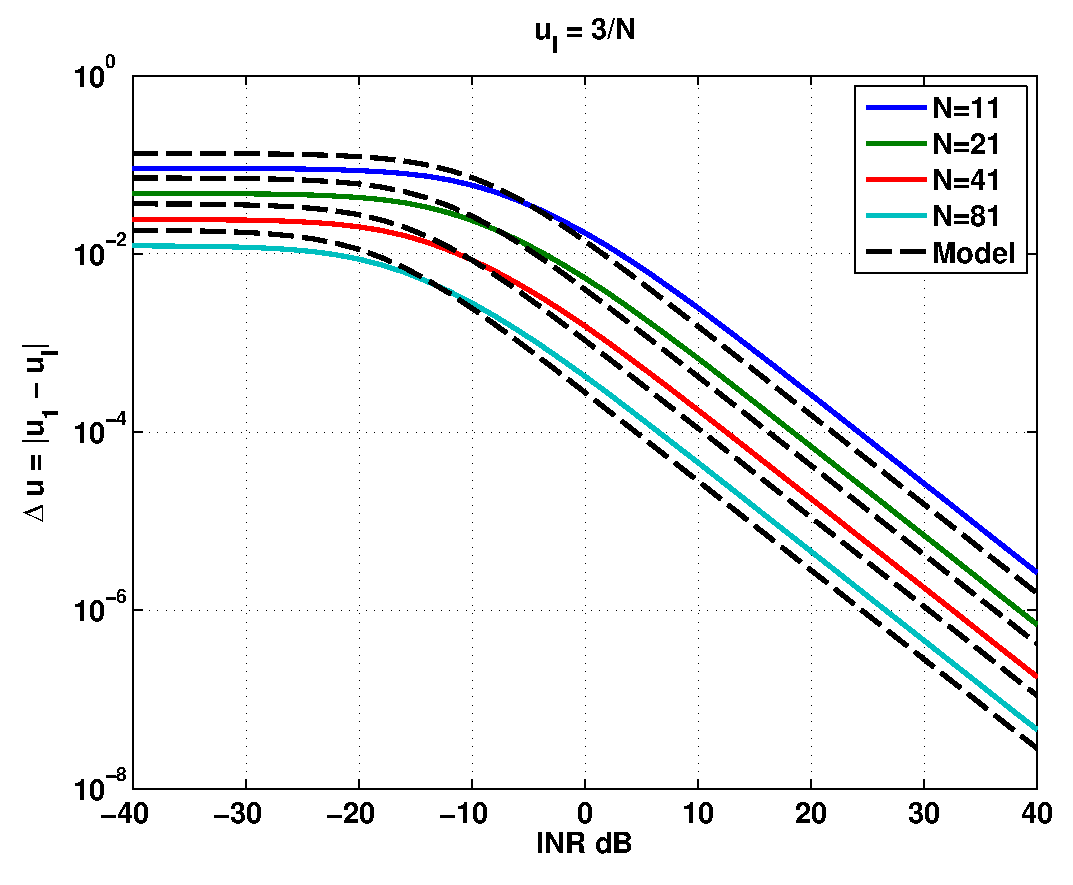
\includegraphics[width=3.5in]{zero_pertb_true_model_ulook1}%
\label{fig:compare_first_case}}

\subfloat[]{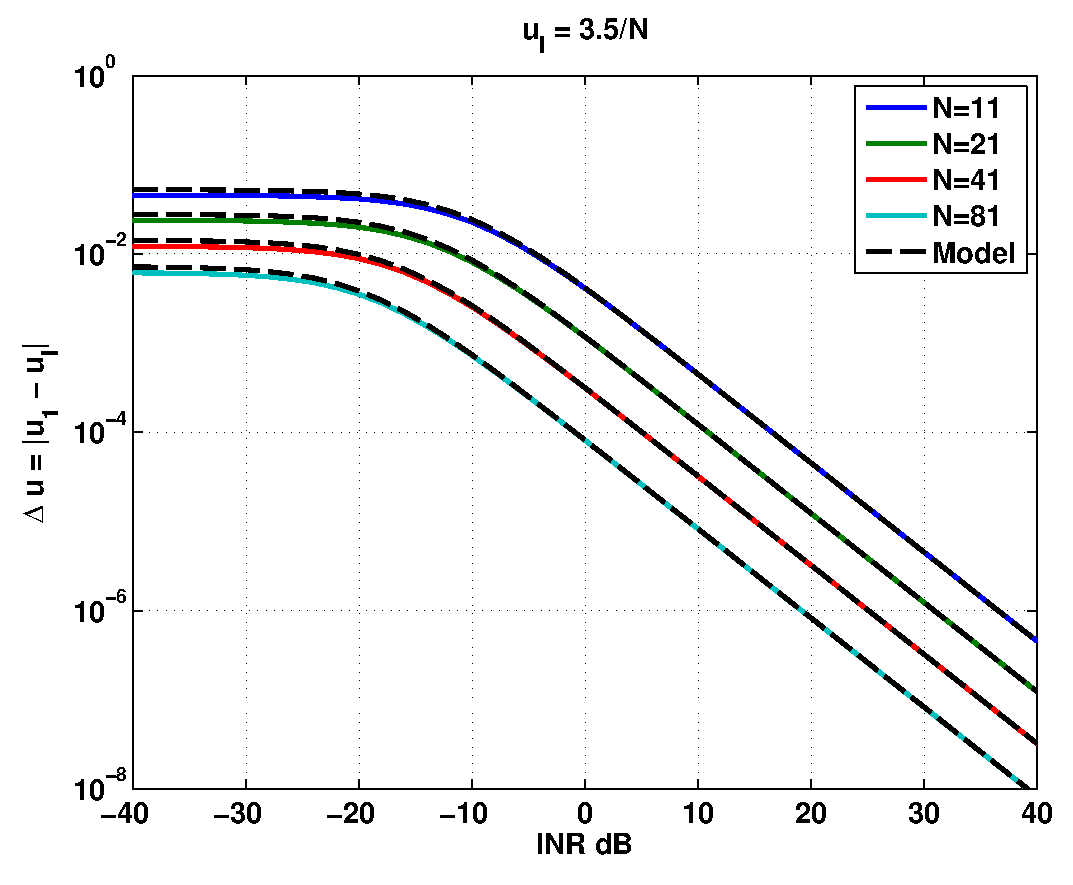
\includegraphics[width=3.5in]{zero_pertb_true_model_ulook2}%
  \label{fig:compare_second_case}}
\caption[Comparison between the actual and the model predicted values
  of the phase angle perturbation $\deltau$]{Comparison between the actual and the model predicted values
  of the phase angle perturbation $\deltau$ when the interferer is
  present at (a) $\uinter = 3/N$ and (b) $\uinter = 3.5/N$. The model
  gives a good prediction of the actual perturbation values.}
\label{fig:model-true-compare}
\end{figure*}

\section{SMI MVDR ABF polynomial}
\label{sec:smi-poly}
The SMI MVDR ABF is the practical realization of the ensemble MVDR
ABF. Each realization of the SMI MVDR ABF has an array polynomial
representation $\smipoly = \ztrans(\wsmi\herm)$. Factoring the SMI
MVDR ABF polynomial in terms of its zeros
\[
\smipoly = G\prod\limits_{n = 1}^{N-1}(1 - \sampz_nz\inv),
\]
where $G$ is a scaling factor ensuring unity gain in the look
direction ($\ulook$), i.e., $P_S(\expo{j\pi\ulook}) = 1$ and
$\sampz_n$ is the $n\nth$ zero. The SMI MVDR ABF polynomial zeros
($\sampz_n$) will be referred to as sample zeros in the sequel. Each
realization of the SMI MVDR ABF produces a new set of $N-1$ sample
zeros. In addition, the sample zeros ($\sampz_n$) do not necessarily
fall on the unit circle, unlike the ensemble zeros ($\ensz_n$) as
described in \sect{}~\ref{sec:mvdr-interf-suppr}.

Numerical experiments show that the sample zeros ($\sampz_n$) are
randomly perturbed from the ensemble zeros ($\ensz_n$) on the complex
plane. \figurename{}~\ref{fig:smi-mvdr-pzplot} shows sample zeros
(green markers) obtained from 1000 independent realizations of the SMI
MVDR ABF. The blue circle markers denote the ensemble zero
locations. The ABF is implemented using a $N = 11$ sensor ULA and
$L = 110$ snapshot data. A single interferer is present at
$\uinter = 3/N$ with $40$ dB INR. Each green marker denotes one of the
ten sample zeros generated from each realization of the SMI MVDR
ABF. The sample zeros cluster around the ensemble zero locations while
not necessarily falling on the unit circle. The sample zeros appear to
be a zero mean perturbation of the ensemble zero locations, although
no analytical characterization is presented here. The number of
snapshots considered in the example is impractically large for passive
sonar scenario, but it is chosen to enhance the clustering of the
sample zeros around the ensemble locations.

The sample zeros located away form the unit circle do not produce
beampattern nulls. Following the analogy with the DT LTI filters, the
sample zeros that fall away from the unit circle produce shallow
troughs instead of deep nulls in the beampattern. Moreover sample
zeros that fall closer to the origin or far outside the unit circle
have negligible contribution to beampattern
\cite[Chap.~5]{Oppenheim1989}. Hence SMI MVDR ABF suffers from high
sidelobes and a distorted mainlobe in the beampattern. Consequently,
the SMI MVDR ABF loses ability to suppress interferers and white
noise. The following chapter describes how the SMI MVDR ABF can be
modified to improve interferer suppression by projecting the sample
zeros to the unit circle.

%% Add this later after JRB approves other detail
% The SMI MVDR ABF converges in probability to the ensemble
% MVDR ABF as the number of snapshots $L$ increases
% \cite{richmond2000nulling}. This implies that the sample zeros
% converge to ensemble zero locations as the number of snapshot
% increases.

\begin{figure}[!hp]
  \centering
  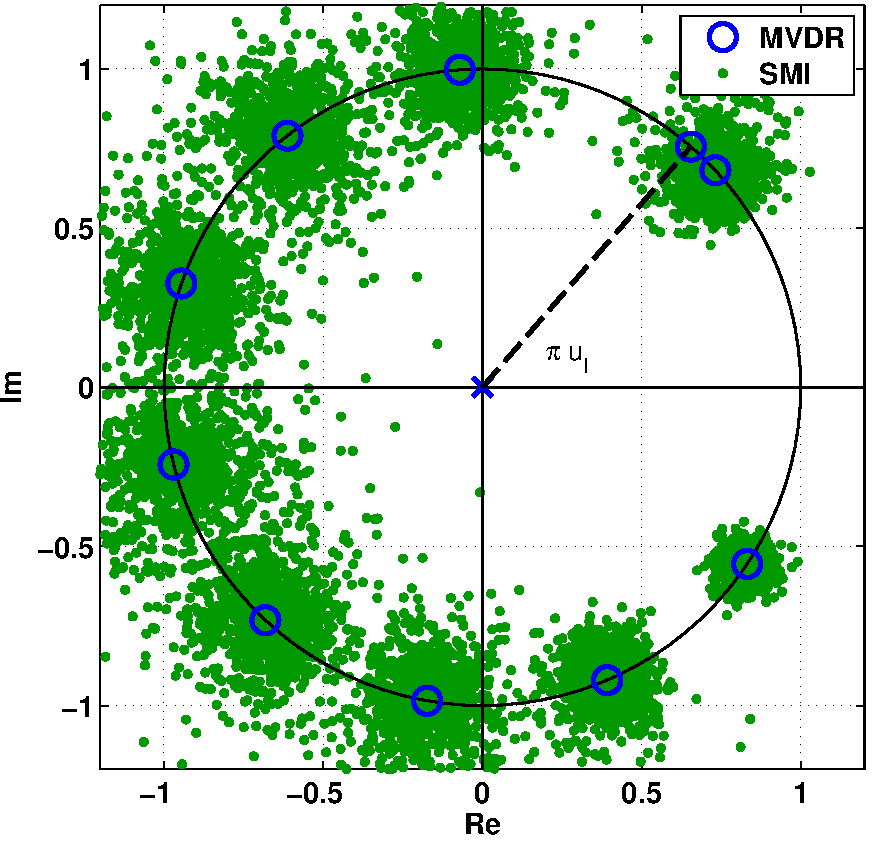
\includegraphics[width=5in]{mvdr_smi_pzlot_N11_L110_INR40}
  \caption[SMI MVDR zeros from 1000 Monte Carlo trials for N = 11, L =
  10 N and INR = $40$ dB]{SMI MVDR zeros from 1000 Monte Carlo trials
    for N = 11, L = 10N and INR = 40 dB. The dashed radial line
    denotes the phase angle associated with the interferer direction
    $\uinter$. The number of snapshots is impractically large for many
    passive sonar situations, but is chosen to create a clearer
    clustering of the SMI zeroes around the ensemble zeroes.}
  \label{fig:smi-mvdr-pzplot}
\end{figure}

%%% Local Variables:
%%% mode: latex
%%% TeX-master: "main"
%%% End:
 % OK
\chapter{Unit circle MVDR ABF}
\label{ch:ucmvdr}
The array polynomial is the $z$-transform of the array weights for a
narrowband planewave beamformer using a ULA as previously discussed in
\ref{sec:array-poly}. Evaluating the array polynomial on the unit
circle in the complex plane yields the beampattern. The locations of
the polynomial zeros on the unit circle indicate the locations of
beampattern nulls. For planewave signals measured with a ULA, the
locations of the ensemble MVDR polynomial zeros are constrained on the
unit circle \cite{steinhardt2004stap,tuladhar2015ucmvdr}. However, the
SMI MVDR polynomial zeros generally do not fall on the unit
circle. This chapter presents the unit circle MVDR (UC MVDR) ABF which
exploits the constraint on the ensemble MVDR polynomial zeros to
modify the SMI MVDR polynomial zeros. The UC MVDR ABF creates deeper
notches and lowers sidelobes on average compared to the SMI MVDR ABF
resulting in better interferer suppression and improved WNG. The first
part of the chapter presents the UC MVDR algorithm. The second part of
the chapter presents the numerical experiment results evaluating the
performance of the UC MVDR ABF. The last part of the chapter discusses
the UC MVDR ABF implementation in a snapshot deficient scenario and
the unit circle DMR ABF implementation. In the sequel, the SMI MVDR
polynomial zeros will be referred to as sample zeros and the ensemble
MVDR polynomial zeros will be referred to as ensemble zeros.

% ====================
% ---------------------
% Algorithm and numerical result discussion included inside "ucmvdr.tex"
% All content from journal submitted to IEEE
\section{UC MVDR algorithm}
\label{sec:ucmvdr-algorithm}
The UC MVDR ABF projects the sample zeros radially on the
unit circle staying consistent with the unit circle constraint on the
ensemble MVDR polynomial zeros. By placing zeros on the unit circle,
the UC MVDR ABF guarantees beampattern nulls in the directions
corresponding to the unit circle zeros. The constraining approach used
by UC MVDR ABF is similar in spirit to ABF approaches which enforce
known structural constraints in the ensemble quantity onto the sampled
data based implementation, e.g., forcing Toeplitz structure when
evaluating the SCM in case of planewave beamforming using ULA
\cite{fuhrmann1991toeplitz}. The rest of the section describes the UC
MVDR algorithm assuming the beamformer is steered towards the
broadside ($\ulook = 0$). The algorithm extends naturally to the case
of a different look direction ($\ulook = u_L$) by rotating all the
zeros to match the look direction.

Algorithm~\ref{alg:ucmvdr} outlines the UC MVDR ABF
implementation. The algorithm begins from the SMI MVDR weights
$\wsmi$. The $z$-transform of the conjugated weights gives the SMI
MVDR polynomial $\smipoly(z) = \ztrans{(\wsmi\herm)}$. Factoring the SMI
MVDR polynomial in terms of the zeros,
\[
\smipoly(z) = G \prod\limits_{n=1}^{N-1}(1 - \sampz_n z\inv),  
\]
where $G$ is a scaling level to ensure unity gain in the look
direction ($\ulook = 0$), i.e., $\smipoly(\expo{j\pi\ulook}) = 1$ and $\sampz_n = r_ne^{j\omega_n}$ is the $n^{th}$ SMI MVDR
polynomial zero. As previously discussed in Sec.~\ref{sec:mvdr-poly},
the sample zeros are not necessarily on the unit circle
and hence the magnitudes $|\sampz_n| = r_n$ of the roots are generally
not unity. The next step is to radially project the SMI MVDR
polynomial zeros $\sampz_n$ to the unit circle. \figurename{}~\ref{fig:ucmvdr-cartoon} illustrates the projection of the sample zeros (diamond markers) to the unit circle where the zeros are denoted with circle markers. Projection yields a
set of unit circle zeros $\ucz_n = e^{j\omega_n}$ denoted by circle
markers. An exception occurs when the sample zeros fall within the CBF
main-lobe region in the complex plane
i.e. $|\operatorname{arg}(\sampz_n)|<2\pi/N$. Projecting such
zeros radially to the unit circle results in nulls inside the
main-lobe of the UC MVDR ABF. A null inside the main-lobe results in
an undesired effect of the main-lobe distortion and drastic loss in
WNG \cite[Sec.~6.3.1]{vtree2002oap}. Rather than radially projecting
to the unit circle, such zeros are moved to the closest CBF
first-null location on the unit circle such that
$\operatorname{arg}(\ucz_n) = \sign(\omega_n){2\pi/N}$ where
$\sign(\cdot)$ is the sign function. Keeping the zeros outside the
main-lobe region ensures the UC MVDR main-lobe remains undistorted.

\begin{figure}[!hp]
\centering
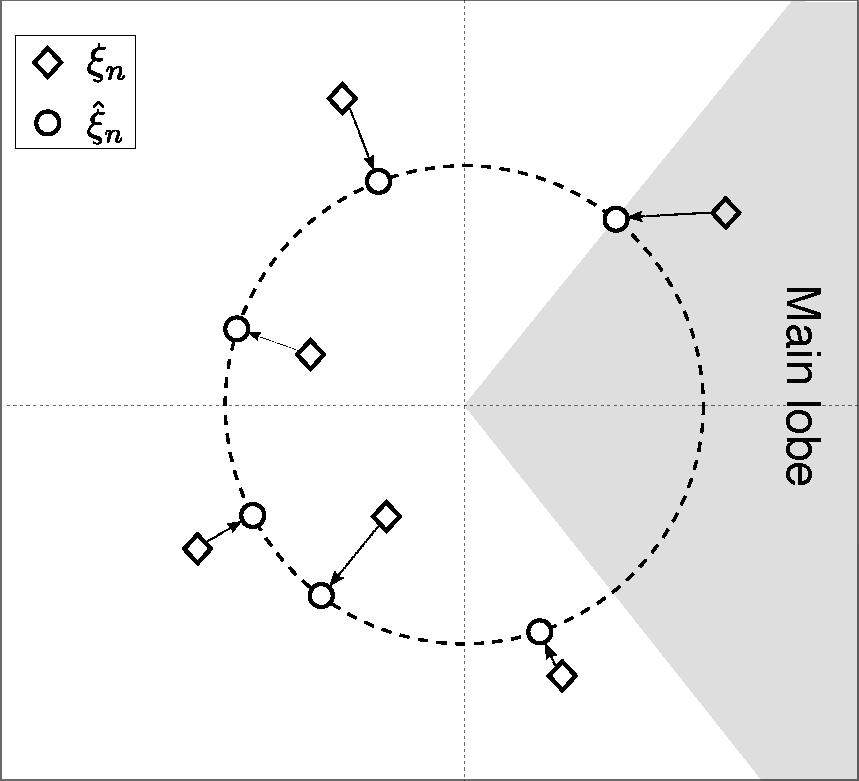
\includegraphics[width=0.9\textwidth]{ucmvdr_cartoon}  
\caption{Schematic shows the unit circle projection technique. The
  diamond markers denote the sample zeros ($\sampz_n$) and the circle
  markers denote the unit circle zeros ($\ucz$) obtained by radially
  projecting the sample zeros. The sample zeros within the main-lobe
  region ($-2/N \leq u \leq 2/N$) are moved to the closest CBF
  first-null location ($u_{\text{null}} = \pm 2/N$) on the unit circle.}
\label{fig:ucmvdr-cartoon}
\end{figure}

The projected unit circle zeros $\ucz_n$ are used to synthesize a unit
circle polynomial
\begin{align}
\label{eq:uc-poly}
\ucpoly(z) =& \prod\limits_{n=1}^{N-1}\frac{(1 - \ucz_n z\inv)}{(1 - \ucz_n)}. \nonumber \\
\intertext{Rewriting the polynomial in terms of the coefficients
}
\ucpoly(z) =& \sum\limits_{n=0}^{N-1} c_n^* z\inv.
\end{align}
Comparing \eqref{eq:uc-poly} to the definition of the array polynomial
\eqref{eq:beampat-poly}, the coefficients $c_n$s can be viewed as
beamformer weights. Thus, the UC MVDR ABF weight vector is defined as
$\wuc = [c_1, c_2, \ldots, c_N]\trans$. Evaluating $\ucpoly(z)$ on the
unit circle produces the UC MVDR ABF beampattern with $N-1$ nulls in
the directions corresponding to $\ucz_n$s and a unity gain in the look
direction ($\ulook = 0$), i.e., $\ucpoly(\expo{j\pi\ulook}) = 1$.

\begin{algorithm}
  \caption{DZ MVDR beamformer} \label{alg:ucmvdr}
  \begin{algorithmic}
    \Procedure{SMI MVDR}{$\datavec{}$}\Comment{Compute SMI MVDR weights}
     \State $\sampCov = \frac{1}{L}\sum\limits_{\ell=1}^L\datavec\datavec\herm$
     \State $\wsmi = {\sampCov\inv\replook}/{(\replook\herm\sampCov\inv\replook)}$
    \EndProcedure
    \Procedure{ProjectUnitCcircle}{$\wsmi$}\Comment{Project zeros to unit circle}
    \State $\smipoly(z) = \ztrans (\wsmi\herm) = G\prod\limits_{n=1}^{N-1}(1 - \sampz_nz\inv)$ 
    \State  $\sampz_n = r_ne^{j\omega_n}$ \Comment{SMI MVDR polynomial zero}
     \If{$|\omega_n| > 2\pi/N$}
     \State $\ucz_n = e^{j\omega_n}$     
     \ElsIf{$|\omega_n| \leq 2\pi/N$}
     \State $\ucz_n = e^{\sign(\omega_n){j2\pi/N}}$
     \EndIf
     \EndProcedure
     \Procedure{UC MVDR}{$\ucz_n$}\Comment{Compute UC MVDR weights}
    \State $\ucpoly(z) = \prod_{n=1}^{N-1}(1 - \ucz_n z\inv)/(1 - \ucz_n) = \sum_{n=0}^{N-1} c_n^*z^{-n}$ 
    \State $\wuc = [c_1, c_2,\ldots,c_N]\trans$
    \EndProcedure
  \end{algorithmic}
\end{algorithm}

%  In order to satisfy the
% distortionless constraint of the MVDR beamformer, the $c_n$s are
% scaled to force unity gain in the look direction. The resulting UC
% MVDR beamformer weight vector is
% $\wuc = {\bf{c}}/{\replook\herm\bf{c}}$ where
% $\mathbf{c} = [c_0, c_1 \ldots c_{N-1}]$ and $\replook$ is the array
% manifold vector for the look direction $\ulook = \cos(\theta_0)$.
% Since the polynomial zeros are invariant to coefficient scaling, the
% UC MVDR beampattern still has nulls in the same locations as the
% polynomial $\ucpoly(z)$.


\figurename{} \ref{fig:smi-ucmvdr-plots} shows a representative
example of the zero locations and the beampattern of a UC MVDR and the
SMI MVDR ABF using an $N = 11$ sensor ULA and $L = 12$ snapshots. Both
ABFs are steered to broadside ($\ulook = 0$) look direction and a
single interferer is present at $\uinter = \cos(\theta_I) = 3/N$. In
\figurename{}~\ref{fig:smi-ucmvdr-pzplot}, the green diamond markers
indicate the SMI MVDR polynomial zero locations and the red circle
markers indicate the UC MVDR zeros projected on unit
circle. \figurename{}~\ref{fig:smi-ucmvdr-bpplot} shows nulls and
lowered sidelobes in the UC MVDR beampattern (solid red) in contrast
to the shallow notches and higher sidelobes of the SMI MVDR
beampattern (dot-dash green). The lowering of the sidelobes reduces
the area under the beampattern magnitude, which in turn improves the
WNG of the UC MVDR as described by \eqref{eq:wng-beampat}.

As discussed in Sec.~\ref{sec:mvdr-poly}, the SMI MVDR polynomial
zeros are randomly perturbed in both magnitude and phase from the
ensemble zero locations on the unit circle. Projecting the SMI MVDR
polynomial zeros back on the unit circle corrects the magnitude
perturbation in the sample zeros thereby satisfying the
ensemble constraint of unit circle zeros. Moreover, the UC MVDR
weights can be seen as the closest approximation of SMI MVDR weights
in the ensemble constraint space, i.e., on the unit circle.

\begin{figure}[!hp]
\centering
\subfloat[Zero locations]
{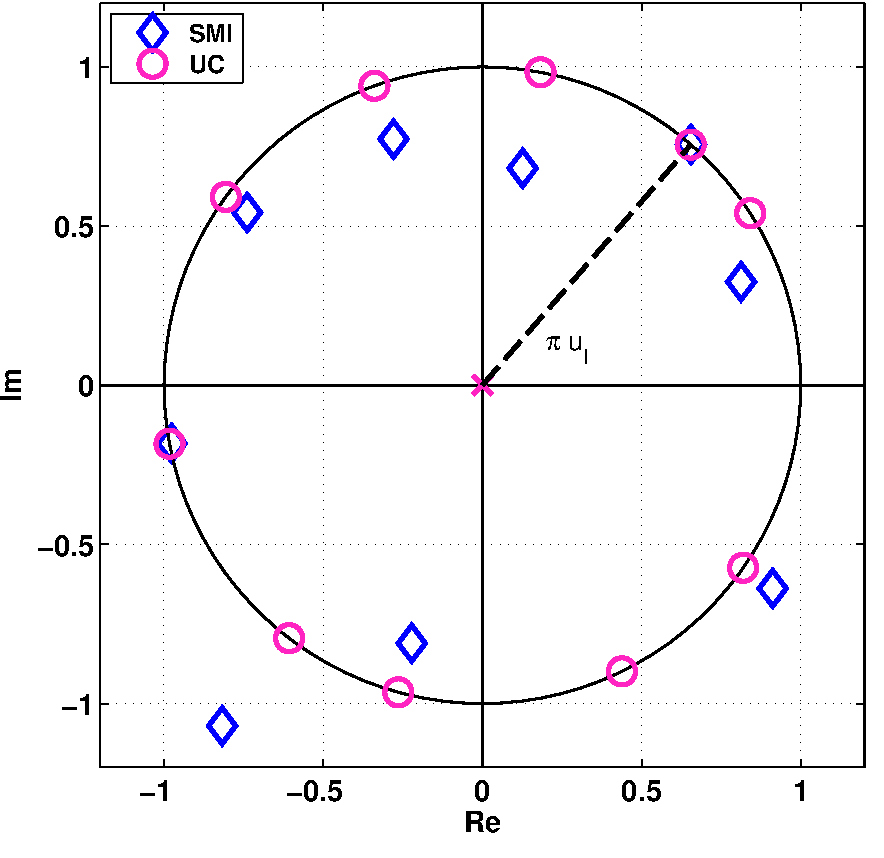
\includegraphics[width=3.5in]{mvdr_smi_dl_zfc_N11_pzplot_eg}  \label{fig:smi-ucmvdr-pzplot}}

\subfloat[Log-magnitude beampattern]{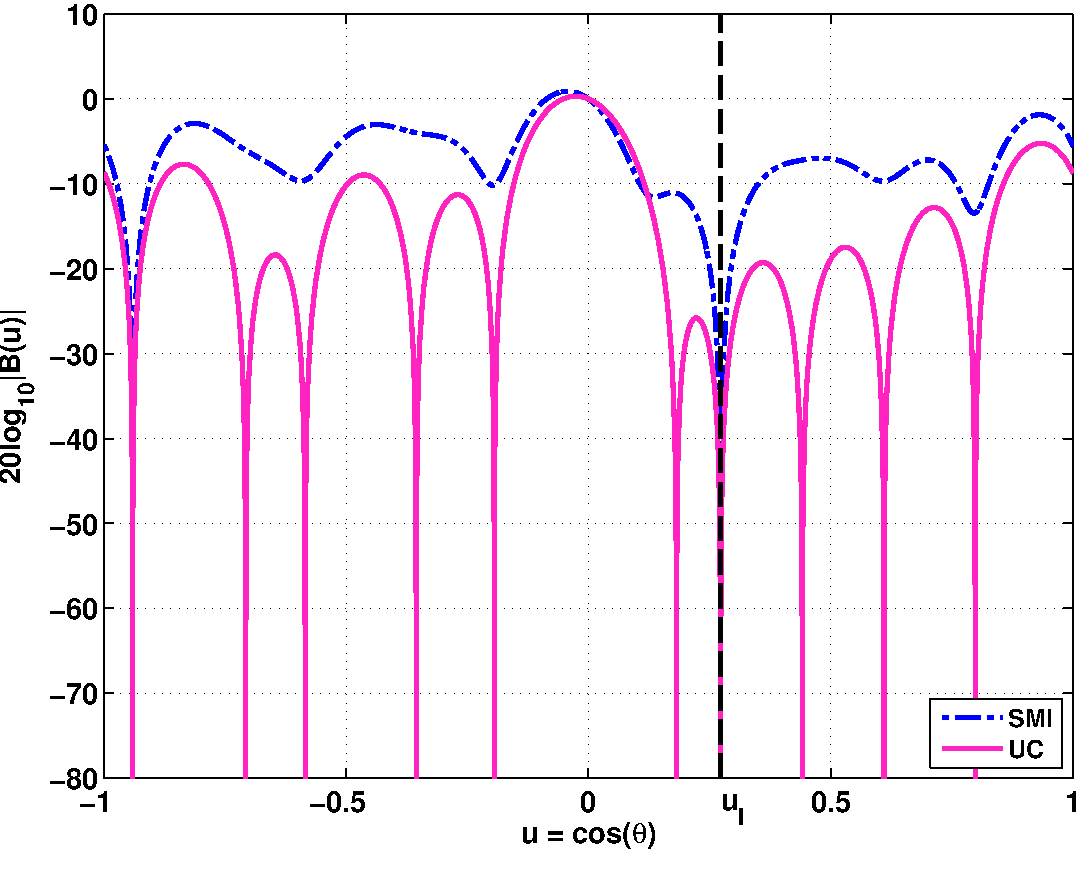
\includegraphics[width=3.5in]{mvdr_smi_dl_zfc_N11_bpplot_eg}  \label{fig:smi-ucmvdr-bpplot}}
\caption{Zero locations and log-magnitude beampatterns of a
  representative example of SMI MVDR (blue) and UC MVDR ABF (magenta)
  using $N = 11$ sensor ULA for $L = 12$ snapshots and look direction
  $\ulook = 0$. The unit circle zeros of the UC MVDR ABF produce nulls
  and lowers sidelobes compared to the SMI MVDR ABF beampattern.}
\label{fig:smi-ucmvdr-plots}
\end{figure}

%%% Local Variables: 
%%% mode: latex
%%% TeX-master: "main"
%%% End: 

\section{Simulation results}
\label{sec:ucbf-perf}
This section presents results of the simulation experiments evaluating
the performance of the UC MVDR ABF compared to the SMI MVDR and the DL
MVDR ABFs. All ABFs are implemented using $N = 11$ and $N = 51$
element ULAs and steered to the broadside look direction($\ulook =
0$). The experiments assume a passive sonar environment where the ABFs
often operate with barely sufficient snapshots $L = N + 1$ and two
snapshots per sensor $L = 2N$ is considered a snapshot rich scenario
\cite{cox2002adaptive,baggeroer1999passive}. The simulated snapshot
consists of a single loud interferer present at $\uinter = 3/N$ and a
unit power white background noise. For such measurement scenario, the
ABF output power $\pout$ is a sum of interferer contribution $\pinter$
and noise contribution $\pnoise$ as discussed in
\sect{}\ref{sec:output-power}. In the sequel, the two components of
the output power are referred to as the interferer output power
($\pinter$) and white noise output power
($\pnoise$). \sect{}\ref{sec:ucmvdr-interf-outp-result} compares the
interferer output power of the ABFs and
\sect{}\ref{sec:ucmvdr-wng-result} compares the WNGs of the
ABFs. Since the white noise output power is determined by the WNG, it
is sufficient to compare the WNGs of the ABFs. All the results are
averaged from a 3000 trial Monte Carlo experiment.

% The ABF output power is computed
% as $\pout = \wthat\herm \Cov \wthat$ where $\wthat$ is the ABF weight
% vector. Using the definition of the ECM for the single interferer case
% the output power is
% $\pout = \cov_I^2|\wthat\herm \rep_I|^2 + \cov_w^2||\wthat||^2 =
% \cov_I^2 \notchdepth + \cov_w^2 {\rm WNG}\inv = \pinter + \pnoise$.
% The total output power is the sum of interferer contribution
% ($\pinter$) and the white noise contribution ($\pnoise$).

%%% TODO
% JRB Comments
% Explain steps in order: first run UC MVDR trials, compute average WNG, then iterate estimating DL level for DL MVDR to match WNG.  Makes it clearer why you can't necessarily predict this.  

% We need to address Mestre DL algorithm at some point.  That really is the best existing benchmark, at least until Milutin Pajovic's papers are published.   

To ensure a fair comparison between the UC MVDR ABF and the DL MVDR
ABF, the DL level ($\dl$) can be chosen to match either the average
WNGs or the average notch depths (ND) between the two ABFs. In the
experiments, the DL level is chosen to match the average WNG between
the UC MVDR and the DL MVDR ABF. In order to determine the DL level,
the experiments first implement the UC MVDR for all trials and compute
the average WNG of the UC MVDR ABF. The DL level is then estimated
iteratively to match the average WNG between the UC MVDR and DL MVDR
ABFs.


\subsection{Interferer output power}
\label{sec:ucmvdr-interf-outp-result}
\figurename{}~\ref{fig:ecdf-plots} shows the empirical cumulative
distribution function (ECDF) of the interferer output power
($\pinter$) for the UC MVDR ABF compared to the SMI MVDR and DL MVDR
ABFs. The upper two panels show the ECDF graphs for the $N = 11$
sensor ULA and the lower two panels show the ECDF graphs for the $N =
51$ sensor ULA. The left two panels show the limited snapshot cases
where $L = N + 1$ and the right two panels show the snapshot rich case
where $L = 2N$. For all ULA sizes and snapshot cases, the sensor level
INR was set at $40$ dB. The dashed vertical line represents the
ensemble interferer output power $\pinter$ obtained from the MVDR
beamformer implemented using the ECM. The interferer output power
$\pinter$ corresponding to the ECDF equal to $0.5$ defines the median
value. The closer the median of the interferer output power $\pinter$
of the ABFs is to the dashed vertical line, higher the better the
probability of producing output comparable to the ensemble case. For
all four cases examined, the DL level for the DL MVDR ABF is chosen to
match the average WNGs as described earlier.

Over the observed interferer output power range in
\figurename{}~\ref{fig:ecdf-plots}, the UC MVDR ABF exhibits
higher probability of achieving lower interferer output power
$\pinter$ compared
against both SMI MVDR and DL MVDR ABFs. For instance in
\figurename{}~\ref{fig:ecdf_N11L12INR40} the median output power of UC
MVDR was approximately 20 times lower than SMI MVDR and 10 times lower
than DL MVDR ABF. The DL MVDR has improved interferer
suppression over SMI MVDR as expected, but UC MVDR has improved
performance compared to both SMI MVDR and DL MVDR ABFs.

\begin{figure}[!hp]
  \centering
  \subfloat[N = 11, L = 12]{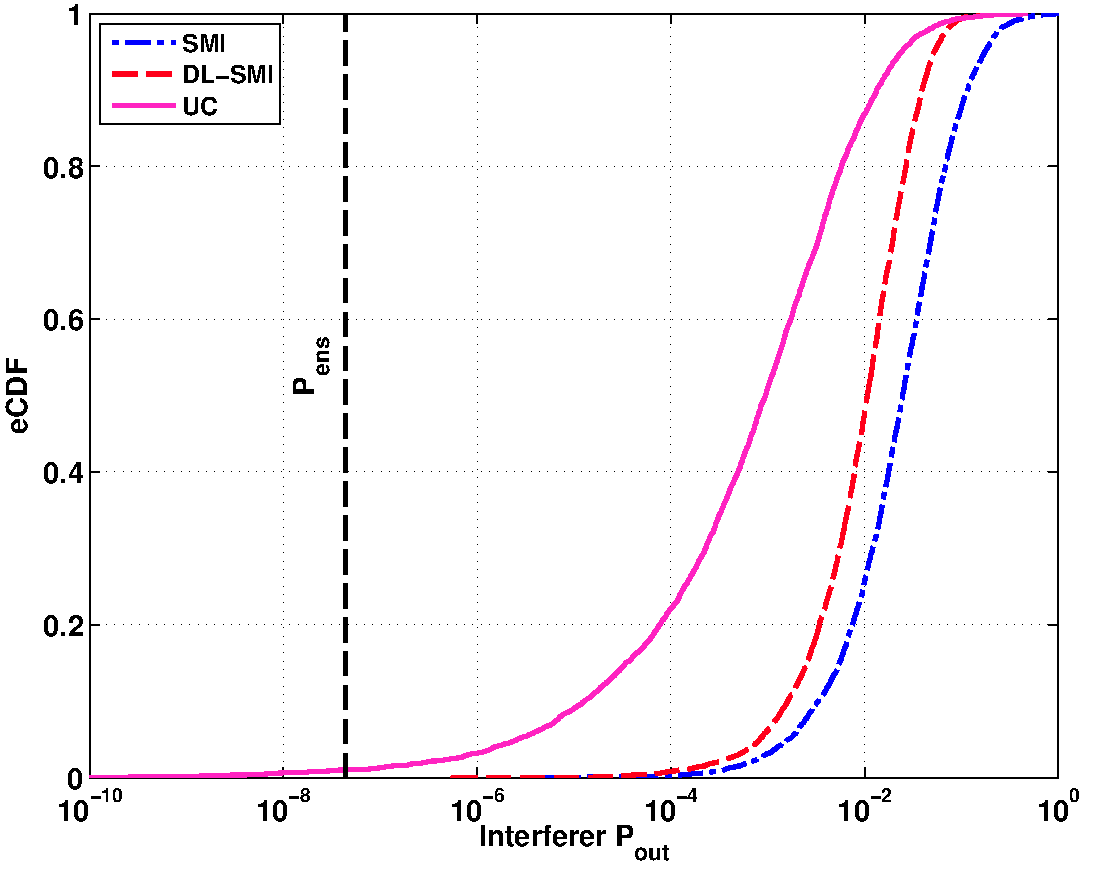
\includegraphics[width=3in]{mvdr_smi_zfc_dl_Po_ecdf_N11L12_INR40}%
    \label{fig:ecdf_N11L12INR40}}
  \subfloat[N = 11, L = 22]{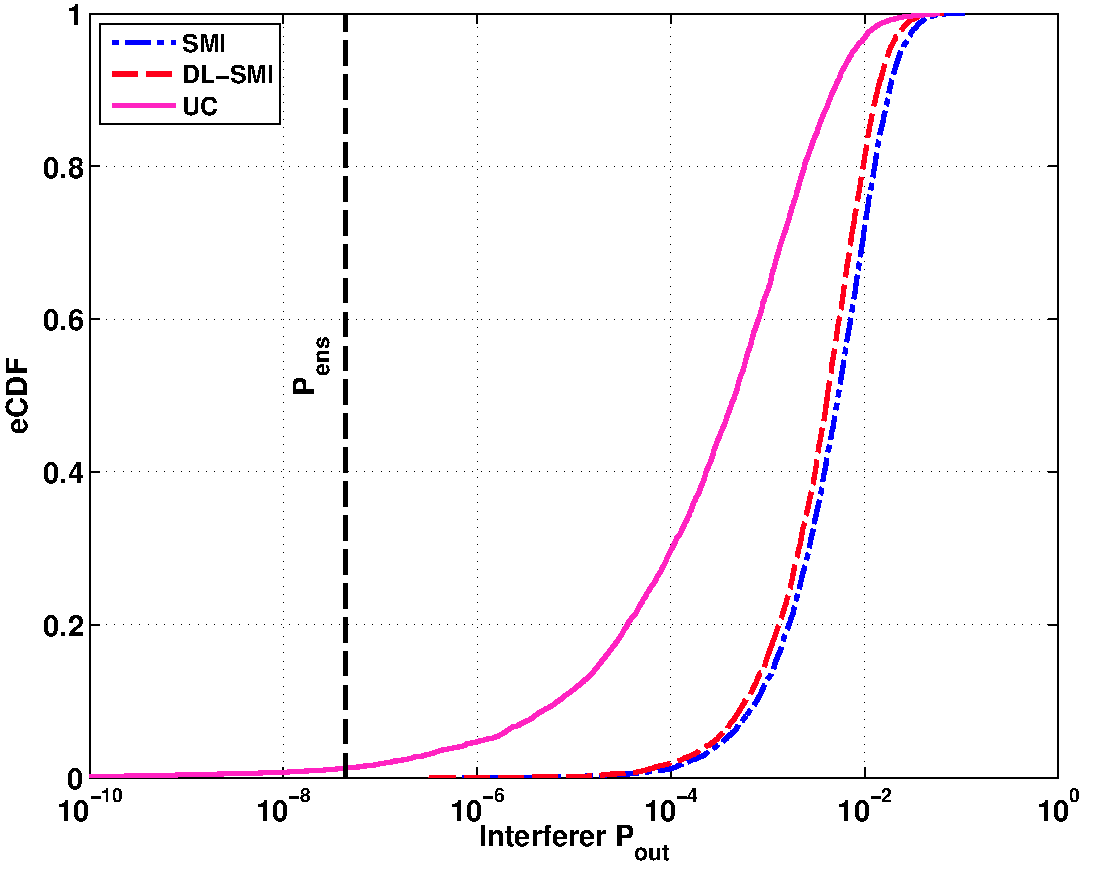
\includegraphics[width=3in]{mvdr_smi_zfc_dl_Po_ecdf_N11L22_INR40}%
    \label{fig:ecdf_N11L22INR40}}\\
  \vfill
  \subfloat[N = 51, L = 52]{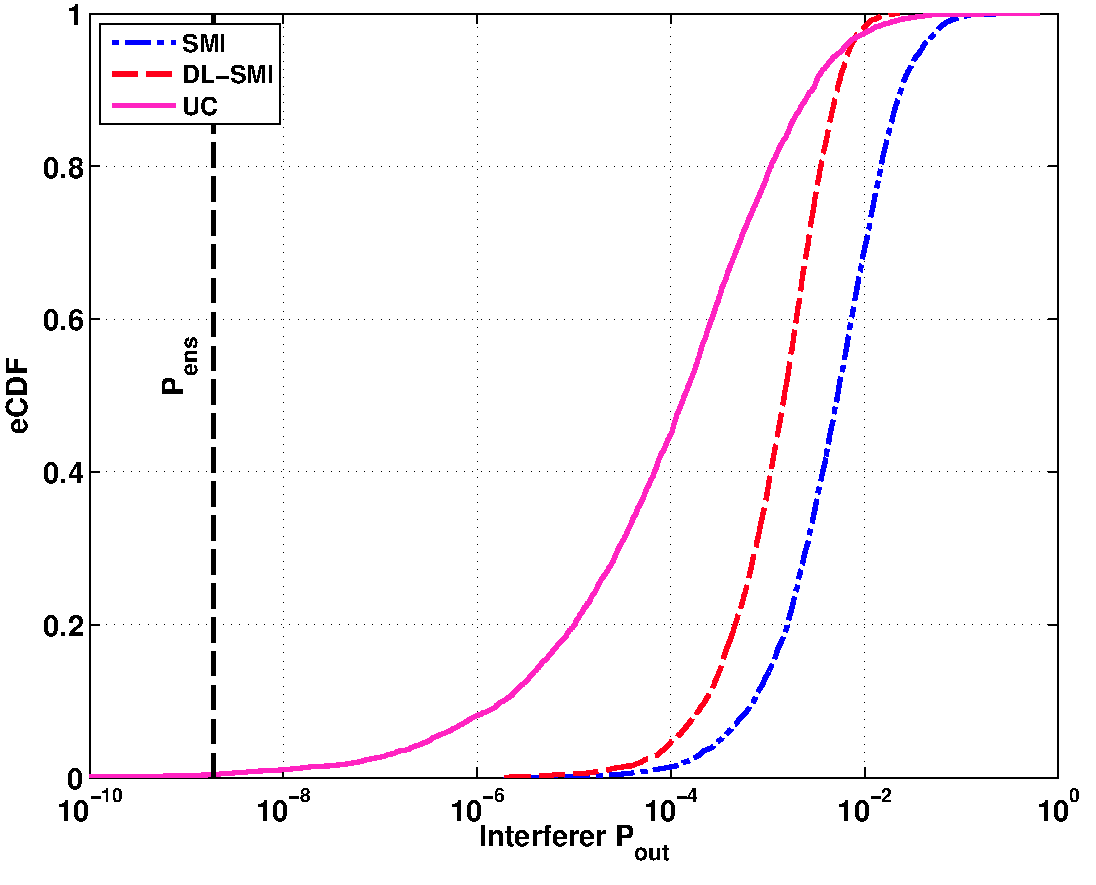
\includegraphics[width=3in]{mvdr_smi_zfc_dl_Po_ecdf_N51L52_INR40}%
    \label{fig:ecdf_N51L52INR40}}
  \subfloat[N = 51, L = 102]{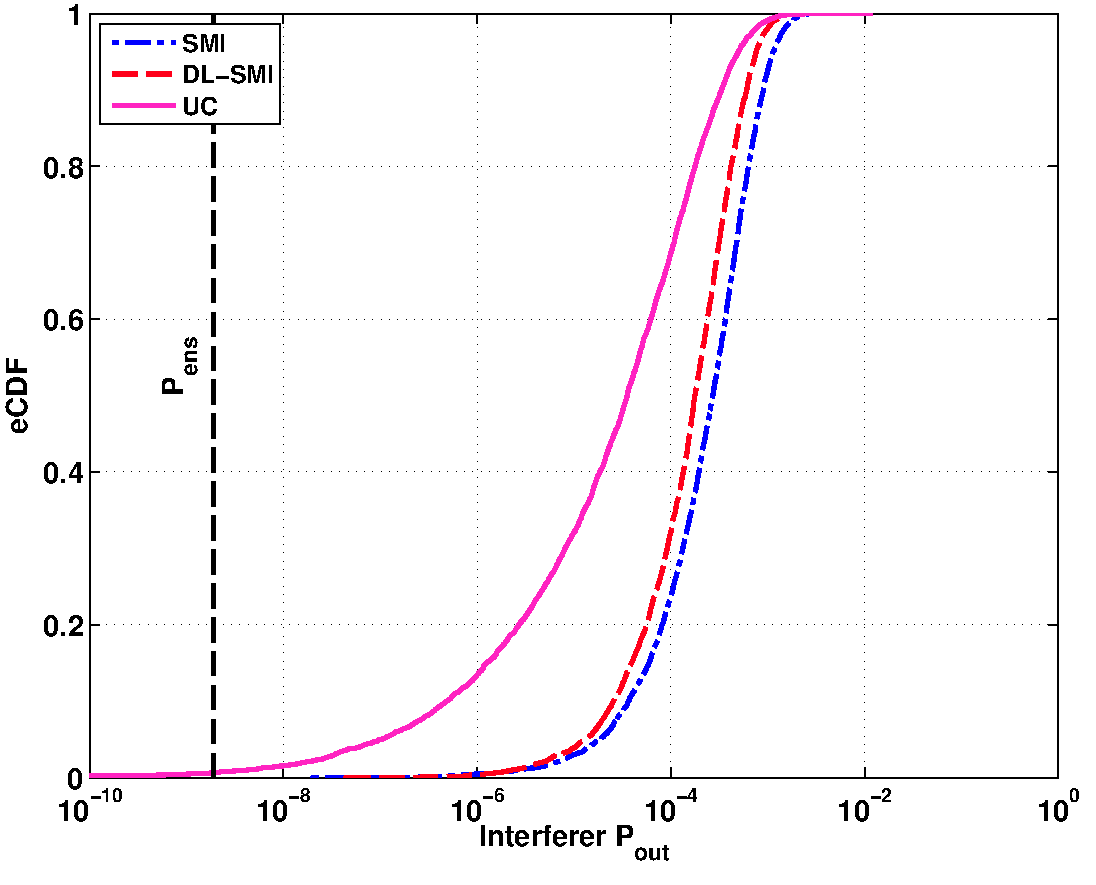
\includegraphics[width=3in]{mvdr_smi_zfc_dl_Po_ecdf_N51L102_INR40}%
    \label{fig:ecdf_N51L102INR40}}
  \caption[Comparison of the ECDF of the interferer contributed output
  power.]{ ECDF of the interferer contributed output power
    $\pinter$. The ECDFs are compared between the SMI MVDR, DL MVDR
    and the UC MVDR ABFs. The ABFs use $N = 11$ element ULA in the top
    panel and $N = 51$ element ULAs in the bottom panel. The left
    panels shows the snapshot deficient case ($L = N + 1$) and the
    right panels shows the snapshot rich case ($L = 2N$). In each
    panel the dashed vertical line denotes the interferer contributed
    output power for the ensemble MVDR ABF. In all cases, the UC MVDR
    ABF suppresses the interferer better compared to the SMI MVDR and
    DL MVDR ABFs.}
  \label{fig:ecdf-plots}
\end{figure}

\figurename{}~\ref{fig:pout-mean-var-plots} compares the squared mean
(solid) and variance (dashed) of interferer output power $\pinter$ for
UC MVDR and SMI MVDR ABFs over a range of INR values from 0 dB to 40
dB. The interferer output power $\pinter$ of the UC MVDR ABF has lower
mean and variance compared to the interferer output power $\pinter$ of
the SMI MVDR ABF. The reduced mean interferer output power $\pinter$
using UC MVDR supports the earlier conclusion that UC MVDR ABF
provides improved interferer suppression. The reduced variance on
interferer output power suggests the UC MVDR ABF should achieve better
detection performance as well.

\begin{figure*}[!hp]
  \centering
  \subfloat[L = 12 snapshots]
{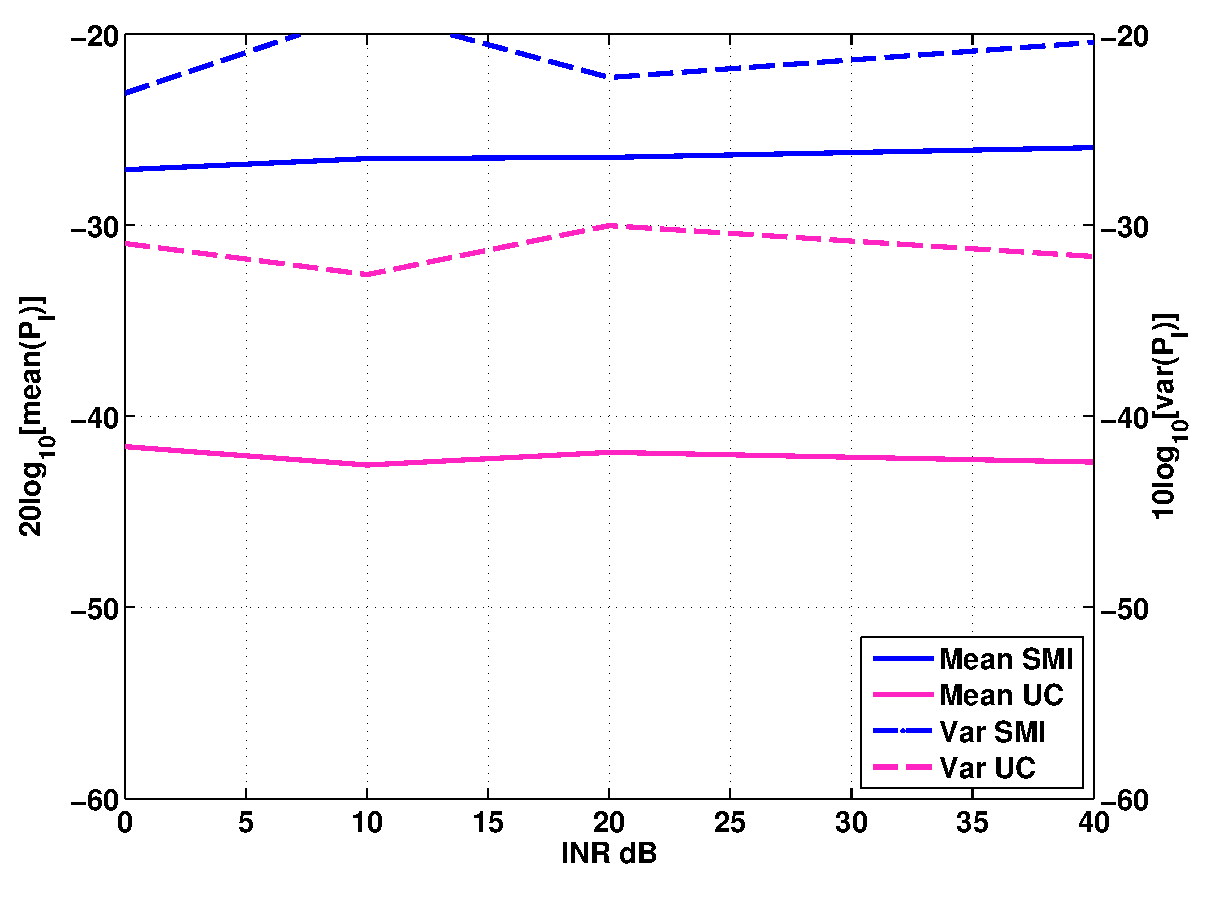
\includegraphics[width=4in]{mvdr_smi_zfc_Po_meansq_var_N11_L12}%
    \label{fig:mpout_N11L12}}  \hfill
  \subfloat[L = 22 snapshots]
{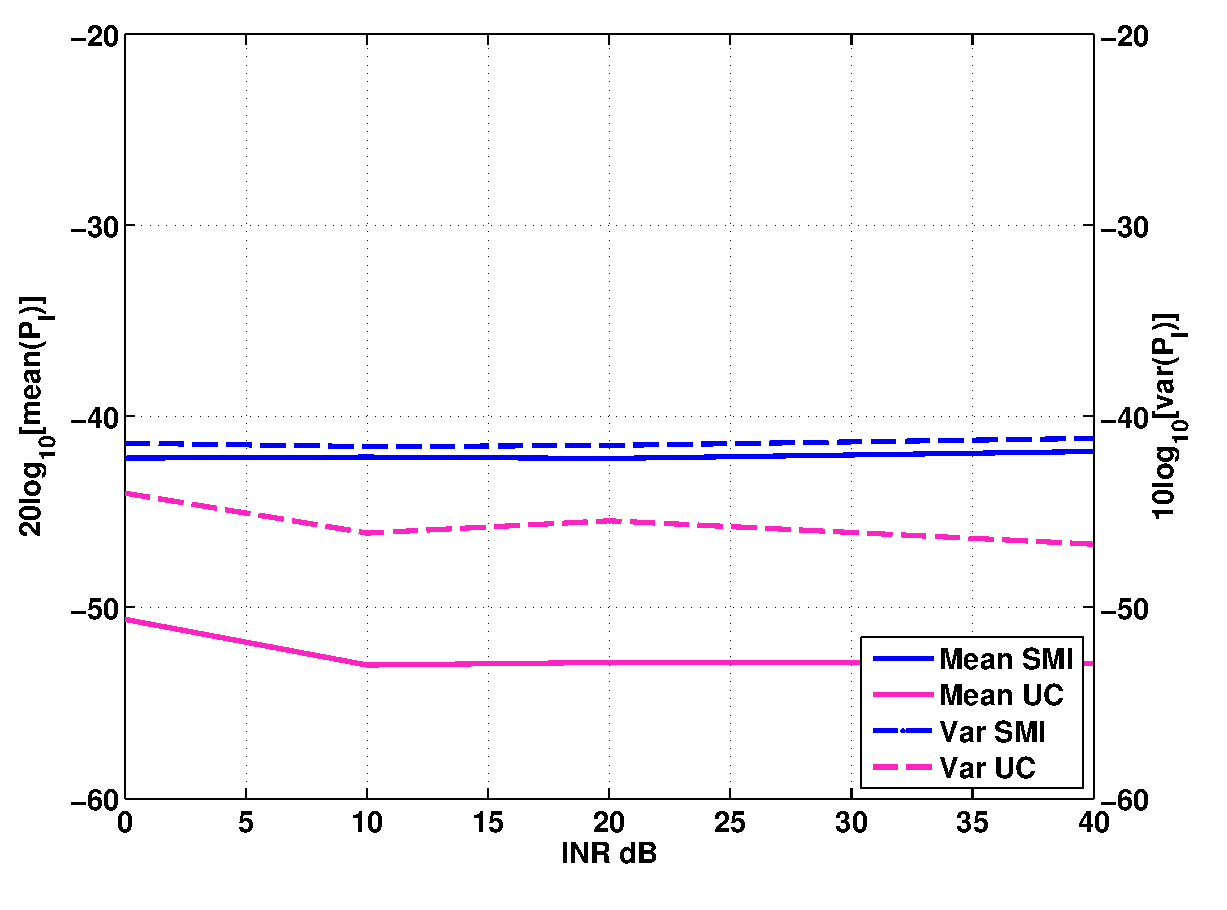
\includegraphics[width=4in]{mvdr_smi_zfc_Po_meansq_var_N11_L22}%
    \label{fig:mpout_N11L22}}
  \caption{Dual y-axis plot of mean and variance of interferer output power $\pinter$ for the SMI MVDR (blue) and the UC MVDR ABF (magenta). Both ABFs are implement using $N = 11$ element ULA and SCM computed from $L = 12$ snapshots in top panel and $L = 22$ snapshots in bottom panel. The UC MVDR ABF yields interferer contributed output power with lower mean and variance compared to the SMI MVDR ABF.}
  \label{fig:pout-mean-var-plots}
\end{figure*}

\subsection{White noise gain}
\label{sec:ucmvdr-wng-result}
\figurename{}~\ref{fig:wng} compares the WNG of the UC MVDR and the
SMI MVDR ABF implemented using $N = 11$ sensor ULA and $L = 12$
snapshots. The maximum WNG for this experiment is $N = 11$ and
corresponds to the CBF
\cite{vtree2002oap}. \figurename{}~\ref{fig:wng-hist-plot} compares
the histograms of the WNG for the UC MVDR and SMI MVDR ABFs. The UC
MVDR ABF achieves improved WNG compared to the SMI MVDR ABF. The
dashed vertical line denotes the ensemble WNG of $10.473$. The UC MVDR
ABF has a greater probability of achieving higher WNG with an average
WNG of $5.672$ compared to an average WNG of $2.629$ using the SMI
MVDR ABF.

\figurename{}~\ref{fig:wng-scatter-plot} is a scatter plot of the WNG
for the UC MVDR and the WNG for the SMI MVDR ABF. Each point in the
scatter plots the WNG of the UC MVDR ABF against the WNG of SMI MVDR
ABF for a single realization of the ABFs in the Monte Carlo
experiment. The scatter plot shows that the UC MVDR has a higher WNG
than SMI MVDR ABF in each trial instance except for small number of
cases (bottom left corner in \figurename{}~\ref{fig:wng-scatter-plot})
where both ABFs have low WNG. Similar results were observed for the
case of $N = 51$ sensor ULA. Thus, on average the UC MVDR ABF has a
higher WNG than the SMI MVDR ABF. In addition of being able to
suppress white noise, the improved WNG implies that the UC MVDR ABF is
also less sensitive to array parameter perturbations
\cite{Gilbert1955,vtree2002oap}.

% Although a DL MVDR is able to achieve a
% specified WNG with a choice of DL level, it requires
% numerically solving for the DL level \emph{a priori} where as UC MVDR improves the
% WNG devoid of such \emph{a priori} requirements.

\begin{figure}[!hp]
  \centering
  \subfloat[]{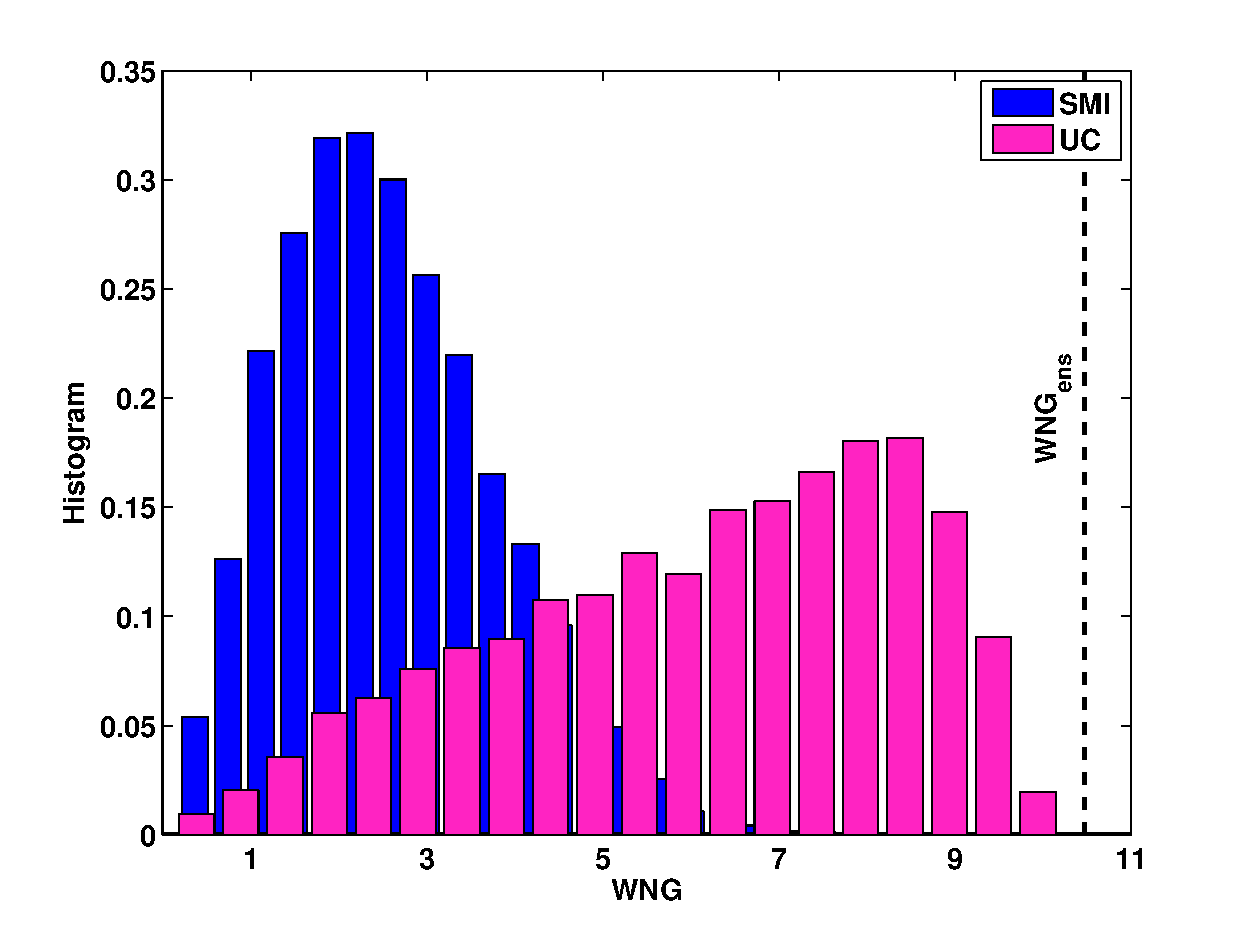
\includegraphics[width=3.5in]{mvdr_smi_zfc_WNG_hist_N11L12_INR40}
    \label{fig:wng-hist-plot}}

\subfloat[]{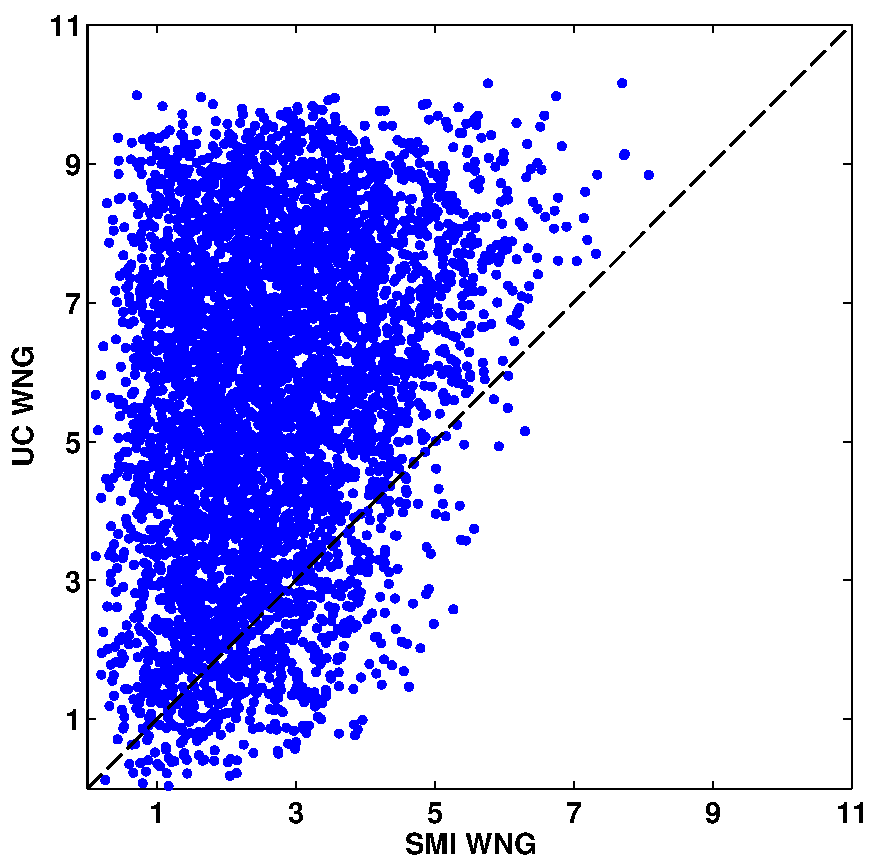
\includegraphics[width=3in]{mvdr_smi_zfc_WNG_scatter_N11L12_INR40}
    \label{fig:wng-scatter-plot}}
  \caption{Comparison of WNG between the UC MVDR and the SMI MVDR ABF,
    both implemented using an $N = 11$ element ULA and $L = 12$
    snapshots. Top panel compares the histogram of WNGs and the lower
    panel is a scatter plot of the WNGs. On average, the UC MVDR ABF
    has higher WNG compared to the SMI MVDR ABF. }
  \label{fig:wng}
\end{figure}

\subsection{UC MVDR and DL MVDR polynomial zeros}
\label{sec:ucmvdr-dlmvdr}
The UC MVDR and the DL MVDR ABF are both derived by modifying the SMI
MVDR ABF. As described above, the UC MVDR ABF moves the sample zeros
radially back on to the unit circle. This section discusses how DL
changes the DL MVDR zeros and compares with the UC MVDR polynomial
zeros.

\figurename{}~\ref{fig:ucbf-dlsmi-pzplot} shows array polynomial zeros
a representative example of ABFs implemented using an $N = 11$ element
ULA and steered to $\ulook = 0$. A single interferer is present at
$\uinter = 3/N$ denoted by the radial dashed line. The blue squares
denote the sample zeros, the magenta circles denote the UC MVDR zeros
and the black diamonds denote the CBF zeros. Each black dot denotes a
DL MVDR zero location as the DL level changes from $-40$ dB to $40$ dB
in $4$ dB steps. When the DL level $\dl \approx 0$, the DL MVDR zeros
are essentially in sample zero locations. As the DL level increases,
the DL MVDR zeros converge towards the CBF zero locations as denoted
by the intermediate dot markers. The intermediate dot markers trace a
trajectory of DL MVDR zero locations starting from the sample zero
location to CBF zero location, as the DL level changes. A specific
trajectory is associated with each sample zero. Hence, changing the DL
level moves the DL MVDR zeros along specific trajectories. As
previously seen in \sect{}\ref{sec:diagonal-loading}, Mestre and
Lagunas present an approach to compute the optimal DL level
\cite{mestre2006finite}. The DL MVDR zeros associated with the optimal
DL level are constrained on the specific trajectories of each sample
zero, and may not be particularly close to the ensemble zero
locations. In fact, any choice of DL level always yields zeros along
the trajectories from sample zero to CBF zero
locations. Comparatively, the UC MVDR ABF approach of moving the
sample zeros radially back to the unit circle is markedly different
approach.

Moreover, one use of applying DL is to improve WNG of the ABFs
\cite{vtree2002oap}. As the DL MVDR zeros move closer to the CBF zero
locations, the WNG performance improves. However, moving zeros closer
to the CBF zero locations leads to loss of ND in the interferer
direction. Hence choosing DL level involves a trade off between loss of
interferer suppression and improved WNG. On the contrary, the unit
circle zeros of the UC MVDR create beampattern nulls which
simultaneously improve notch depth and lower sidelobes. Consequently,
the UC MVDR ABF improves both the interferer suppression and the WNG
performance as discussed in \sect{}\ref{sec:ucbf-perf}. Further, the
UC MVDR ABF does not require choosing a tuning parameter like the DL
level.

% The optimal DL level computed using Mestre and Lagunas
% \cite{mestre2006finite} approach chooses where to stop along the
% trajectory but the trajectories move
% the zeros towards the CBF zero locations instead of the ensemble zero
% locations. The DL MVDR zeros may not be particularly close to the
% ensemble zero locations.  The UC MVDR zeros do not follow the DL MVDR
% zeros trajectory and as seen above improve both WNG and interferer
% suppression.
 

% One benefit of applying DL is that it improves the WNG of the SMI MVDR
% ABF \cite{Gilbert1955}. This improvement in the WNG lowers the
% beampattern sidelobes of the ABF as mentioned earlier in
% \sect{}\ref{sec:wng}. \figurename{}~\ref{fig:ucbf-dlsmi-pzplot} shows
% that the DL MVDR ABF is able to lower the sidelobes by moving the
% polynomial zeros closer to the unit circle. As the zeros move closer
% to the unit circle, the beampattern local minimas become deeper and
% pull down the sidelobes. In contrast, the UC MVDR ABF always projects
% the SMI MVDR polynomial zeros to the unit circle. The unit circle
% zeros ensure nulls in the beampattern and also reduce sidelobes
% improving WNG. Moreover, as discussed earlier the UC MVDR ABF does not
% require an \emph{a priori} choice of a tuning parameter like the DL
% level.

\begin{figure}[!hp]
  \centering
  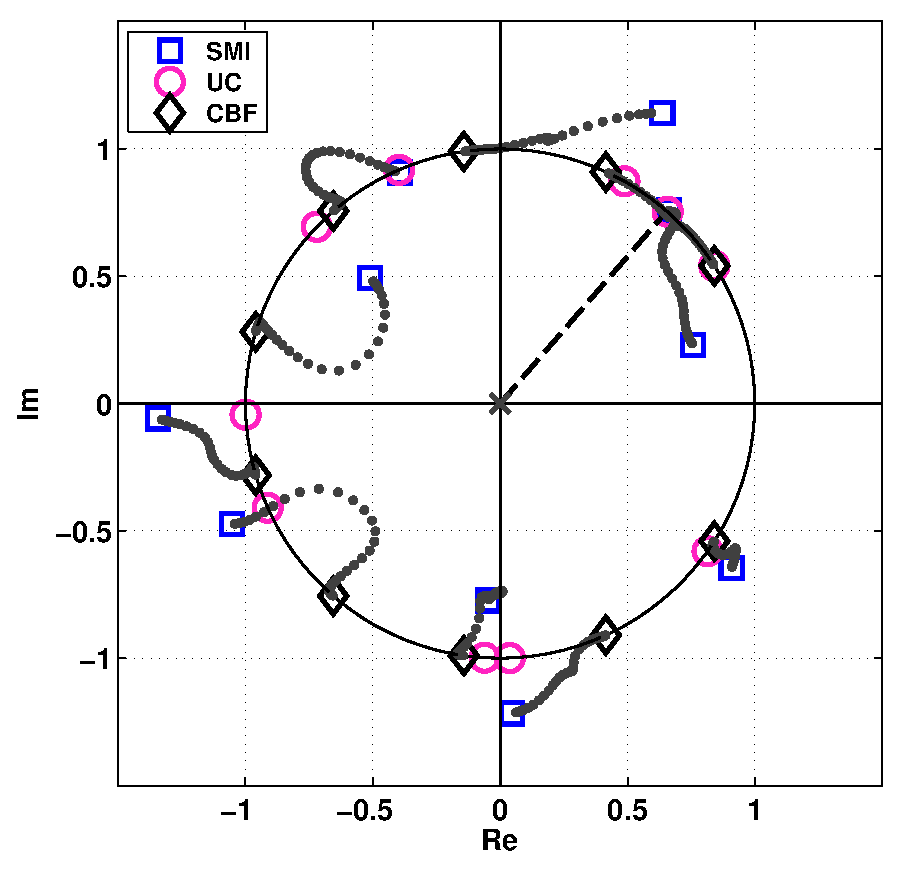
\includegraphics[width=\textwidth]{mvdr_smi_uc_cbf_dl_varying_pzplot}
  \caption{UC MVDR polynomial zeros compared against DL MVDR
    polynomial zeros as the DL level $\dl$ is increased from $-40$ dB to
    $40$ dB. The DL MVDR polynomial zeros asymptotically converge to CBF polynomial zero locations as $\dl \rightarrow \infty$. }
  \label{fig:ucbf-dlsmi-pzplot}
\end{figure}

%%% Local Variables: 
%%% mode: latex
%%% TeX-master: "main"
%%% End: 

% --------------------
% ====================

\section{UC MVDR ABF in snapshot deficient case}
\label{sec:uc-mvdr-snapshot-def}
This section presents one approach to implement the UC MVDR ABF in a
snapshot deficient scenario ($L < N$). The UC MVDR algorithm begins by
initially computing the SMI MVDR weights. However, when snapshot
deficient the SCM is not invertible and hence SMI MVDR ABF cannot be
directly implemented as mentioned in Ch.~\ref{ch:lit-rev}. One common
solution is to apply diagonal loading (DL) to the SCM to make it full
rank and hence invertible. The SMI MVDR weights are then computed
using the full rank DL SCM. The DL level can be chosen using one of the
approaches mentioned in \sect{}\ref{sec:ucbf-perf}. The previous
section discussed the effect of applying DL on the locations of the
sample zeros. When the DL level is small enough the
effect on the SMI MVDR polynomial zero locations is negligible.

In the snapshot deficient scenario, an alternative approach is to
choose a minimal DL level $\dlmin$ just enough to make the SCM
invertible and compute the SMI MVDR weights. The SMI MVDR weights
evaluated using the minimally loaded SCM can be seen as the closest
approximation to the SMI MVDR weights when just enough snapshots are
available ($L \approx N$) to obtain a full rank SCM without having to
apply DL. Following this alternative approach, the proposed
implementation of the UC MVDR ABF in snapshot deficient case begins
with a minimally loaded SCM used to compute the SMI MVDR
ABF. Subsequently the UC MVDR ABF weights are derived by projecting
the sample zeros onto the unit circle as described
previously.

\figurename{}~\ref{fig:ucmvdr-snapshot-deficient} evaluates the UC
MVDR ABF implemented for a $N = 11$ sensor ULA in two snapshot
deficient cases. The top panel corresponds to the case with $L = 10$
snapshots and the bottom panel corresponds to the case with $L = 5$
snapshots. In both panels, the solid magenta curve shows the
interferer output power ECDF graph for the UC MVDR ABF implemented
using a minimal DL level \mbox{$\dl_{min} = 10^{-8}$}. The dot-dashed
red curve shows the interferer output power ECDF graph for the DL MVDR
ABF. The DL level $\dl$ is chosen to match the average WNG with the UC
MVDR ABF. As described in \sect{}~\ref{sec:ucbf-perf}, finding the DL
level for the DL MVDR ABF involves first implementing the UC MVDR ABF
with minimal DL for all trials and computing the average WNG. The DL
level for DL MVDR is estimated iteratively to match average WNG
between the two ABFs. Following this approach, in the top panel use
$\dl = 0.1080$ and in the bottom panel uses $\dl = 0.5856$ for the DL
MVDR ABF. Comparison of the ECDF graphs show that in both snapshot
cases, the UC MVDR ABF exhibits higher probability of suppressing the
interferer compared to the DL MVDR ABF. This implies even in a
snapshot deficient case, on average the UC MVDR ABF implemented using
the minimal DL approach attenuates interferer better than the DL MVDR
ABF.

\begin{figure*}[!hp]
  \centering
  \subfloat[L = 10, $\dl = 0.1080$]
  {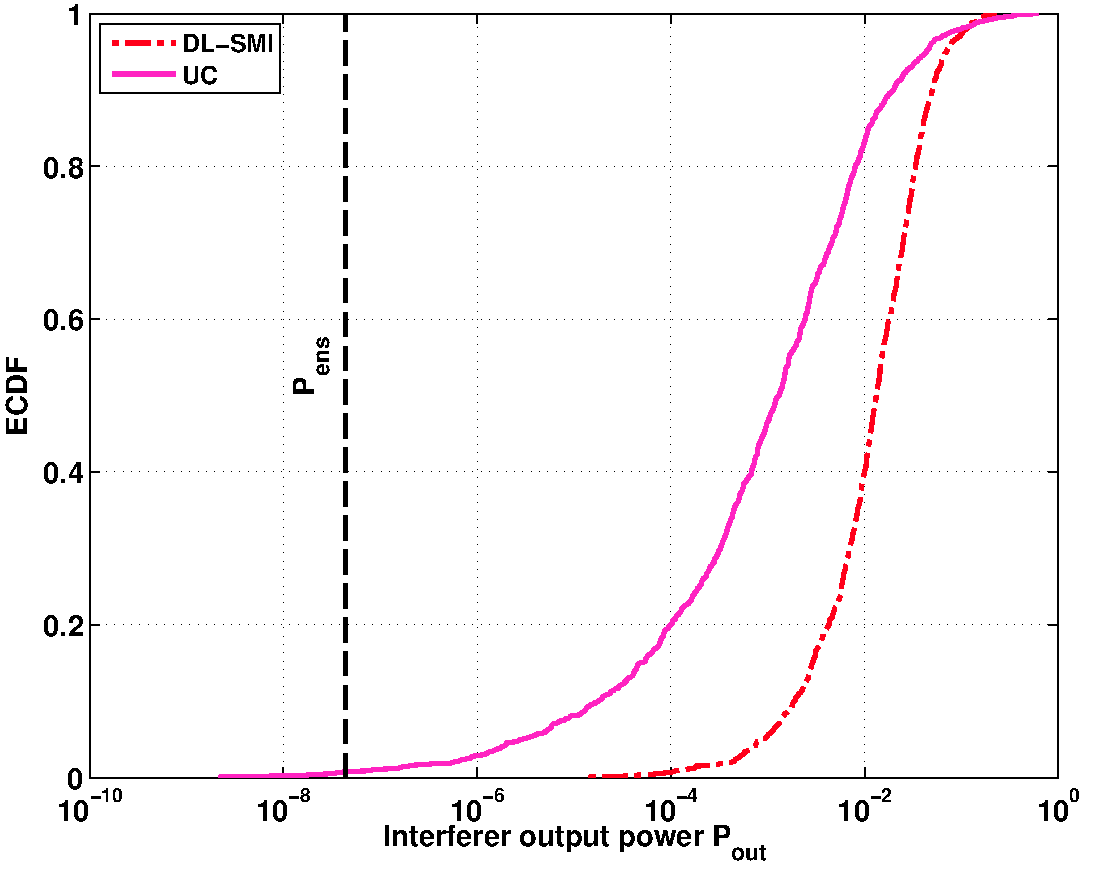
\includegraphics[width=3.5in]{mvdr_dlsmi_uc_ssd_Po_ecdf_N11L10_INR40.pdf}}  

  \subfloat[L = 5, $\dl = 0.5856$]
  {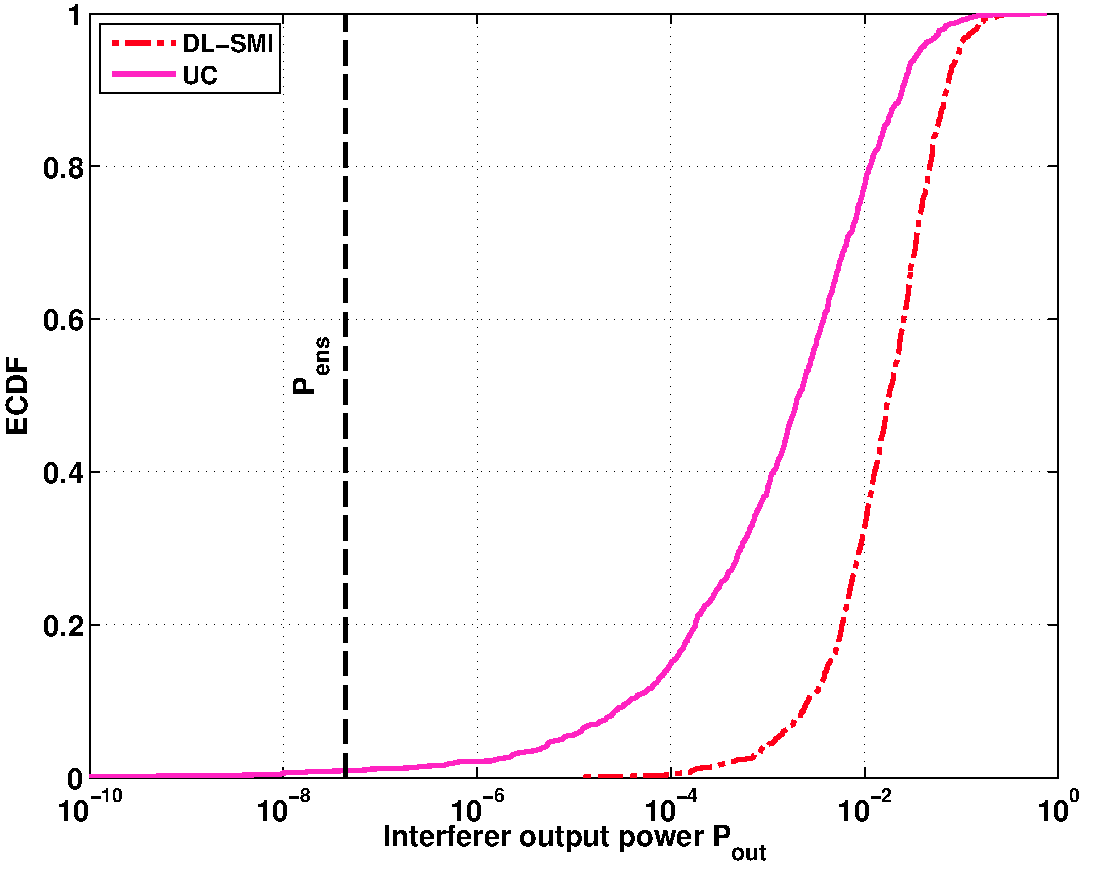
\includegraphics[width=3.5in]{mvdr_dlsmi_uc_ssd_Po_ecdf_N11L5_INR40.pdf}}

  \caption[ECDF of interferer contributed power for the UC MVDR ABF
  and the DL MVDR ABF in a snapshot deficient scenario.]{ECDF of
    interferer contributed output power compared between the UC MVDR
    ABF and the DL MVDR ABF in a snapshot deficient scenario. Both
    ABFs are implemented using $N = 11$ element ULA and the top panel
    considers $L = 10$ snapshots while the bottom panel considers
    $L = 5$ snapshots available to compute SCM. In both cases, the UC
    MVDR ABF uses a minimal DL ($\dl_{min} = 1e^{-8}$) and the DL MVDR
    ABF uses a DL level set to match the WNG with the UC MVDR ABF. The
    UC MVDR }
  \label{fig:ucmvdr-snapshot-deficient}
\end{figure*}

\section{ Unit Circle DMR ABF}
\label{sec:uc-mvdr-dmr}
As previously noted, the DMR ABF is another practical implementation
of the MVDR beamformer. The DMR ABF is almost always implemented using
the SCM. The DMR ABF replaces the SCM in \eqref{eq:mvdr-wt} with the
structured DMR SCM \eqref{eq:dmr-scm} to compute the DMR ABF
weights. The ensemble form of the DMR ABF is essentially the MVDR
beamformer in white background noise. Following a
similar approach as the UC MVDR ABF, a unit circle DMR (UC DMR) ABF is
derived by projecting the DMR polynomial zeros on the unit circle. The
difference from the UC MVDR ABF is that the SCM noise eigenvalues are
averaged implementing the unit circle constraint.
  
\figurename{}~\ref{fig:uc-mvdr-dmr-pout} compares the interferer
output power ECDF of the UC DMR ABF, the UC MVDR and the SMI MVDR
ABF. The ABFs are implemented using $N = 11$ sensor ULA and $L = 12$
snapshots. A single interferer with $40$ dB INR is present at
direction $\uinter = 3/N$. Knowing that only a single interferer is
present, the dominant subspace dimension for the DMR SCM equals to
one. The noise eigenvalue of the DMR SCM is averaged from the $10$
smallest eigenvalues of the SCM. In
\figurename{}\ref{fig:uc-mvdr-dmr-pout}, the top panel compares the
ECDF graphs of the UC MVDR, the UC DMR and the SMI MVDR
ABFs. Comparisons of the output power ECDF graphs show that the UC
MVDR ABF and the UC DMR ABF have comparable ability to suppress
interferer. As expected both the UC MVDR and the UC DMR ABFs perform
better than the SMI MVDR ABF. The bottom panel shows a scatter plot
where each dot marker denotes the WNG of the UC MVDR ABF against the
WNG of the UC DMR ABF. Examining the WNG scatter plot, the WNG of the
UC MVDR ABF is almost always lower than the WNG of the UC DMR ABF. The
WNG of the UC MVDR ABF exhibits high variability while the WNG of the
UC DMR ABF has almost no variability and on average comparable to the
optimal WNG of $N = 11$. Wage and Buck have shown that in case of a
signal strong interferer outside the main-lobe, the WNG of the DMR ABF
has low variability and on average the WNG is close to the optimal WNG
of $N$\cite{wage2013dmr}. The UC DMR ABF inherits the WNG behavior of
the DMR ABF. These results indicate that compared to the UC MVDR ABF,
the UC DMR ABF exhibits similar ability to suppress the interferer
and a better WNG performance. However, the UC DMR ABF is limited by
the need to determine the dominant subspace dimension before
implementing the ABF whereas the UC MVDR ABF is devoid of such prior
requirements.

\begin{figure}[!hp]
  \centering
  \centering
  \subfloat[]
  {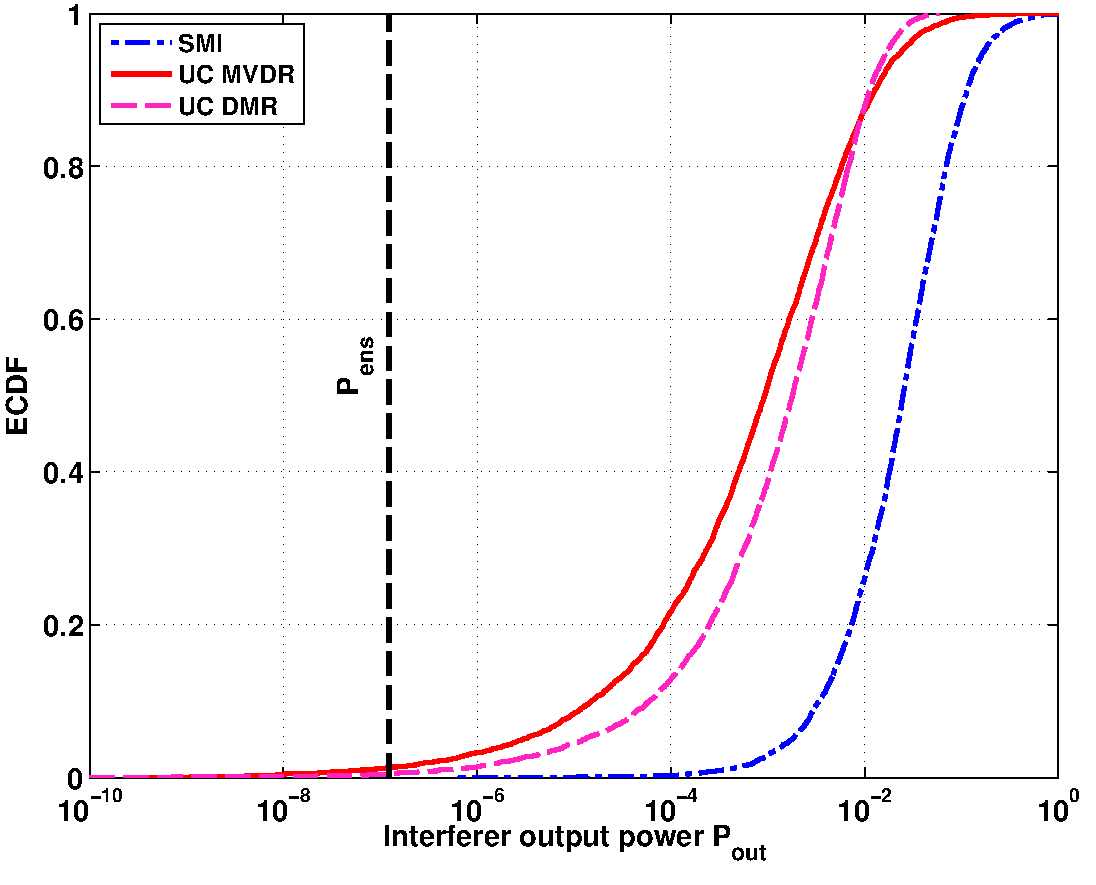
\includegraphics[width=3.5in]{smi_ucmvdr_ucdmr_Po_ecdf_N11L12_INR40.pdf}}  

  \subfloat[]
  {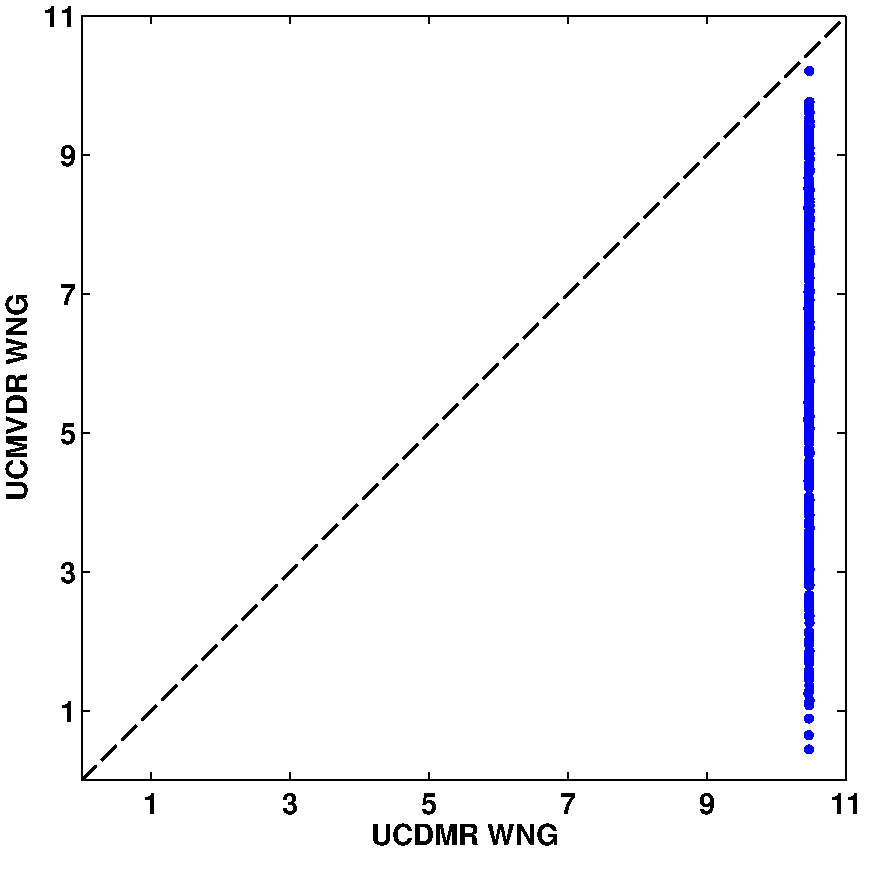
\includegraphics[width=3in]{smi_ucmvdr_ucdmr_WNG_scatter_N11L12_INR40.pdf}}
  \caption[Output power comparison between UC MVDR and UC DMR]{(a)
    ECDF of the interferer contributed output power compared between
    the UC MVDR, UC DMR and the SMI MVDR ABFs. (b) Scatter plot of the
    WNGs of the UC MVDR and UC DMR ABFs. All ABFs are implemented
    using $N = 11$ sensor ULA and $L = 12$ snapshots. The UC DMR attenuates interferer similarly to the UC MVDR ABF and has superior WNG.}
  \label{fig:uc-mvdr-dmr-pout}
\end{figure}

\section{Summary}
\label{sec:ch3-summary}
This chapter presents the UC MVDR ABF which projects the SMI MVDR
polynomial zeros radially on the unit circle to create perfect nulls
in the beampattern. By moving the sample zeros to the
unit circle, the UC MVDR zeros satisfy the unit circle constraint on
the ensemble zeros and creates deeper beampattern notches in the
interferer directions. In a snapshot deficient scenario the UC MVDR
ABF is derived from a SMI MVDR ABF evaluated using a minimally loaded
SCM. Numerical simulations show that the UC MVDR ABF suppresses
interferer better than both the SMI MVDR and DL MVDR ABF. Comparing
the WNG of the ABFs shows that on average the UC MVDR ABF has
higher a WNG than the SMI MVDR. Also, the UC MVDR ABF interferer
suppression is comparable to the UC DMR ABF. However unlike the DL MVDR ABF and the UC DMR ABF both of which requires choosing a design parameter,
the UC MVDR is not constrained to such requirements.
%%% Local Variables:
%%% TeX-master: "main"
%%% End: % OK
\chapter{Double zero MVDR ABF for notch broadening}
\label{ch:dzmvdr}
ABFs encounter interferer direction mismatch because of interferer
motion or limited sample support available to compute the SCM
\cite{vtree2002oap}. This mismatch results in a loss of interferer
suppression and degraded output performance. Notch broadening is a
robust beamforming technique to address interferer mismatch by
creating wider beampattern notch in the interferer direction. This
chapter presents a new ABF approach for notch broadening. The double
zero MVDR (DZ MVDR) ABF exploits the properties of the array
polynomial zeros to create broad notch in the interferer
direction. The DZ MVDR ABF assumes using a ULA similarly to the UC
MVDR ABF, but does not necessarily assume that the observed snapshots are
plane waves. The first two sections of this chapter introduces the
interferer mismatch problem and the notch broadening technique for
robust beamforming. \sect{}~\ref{sec:second-order-zeros} discusses the
behavior of ABF beampattern in the vicinity of a null.
\sect{}\ref{sec:double-zero-mvdr} describes the DZ MVDR
algorithm. \sect{}\ref{sec:results} presents results of experiments
evaluating the DZ MVDR ABF in both stationary and moving interferer
scenarios. The DZ MVDR ABF is compared with the SMI MVDR, the DL MVDR
and the CMT MVDR ABF.

\section{Interferer mismatch}
\label{sec:interferer-mismatch}
ABFs place sharp and deep notches in the expected interferer direction
to suppress interferer power at the output. However in applications
involving interferer motion or limited snapshot support, the ABFs
suffer from interferer mismatch, i.e., the expected interferer
direction is different from the true interferer direction
\cite{vtree2002oap, riba1997comm, baggeroer1999passive}. Due to this
mismatch in interferer direction, the ABFs place a deep notch in a
direction different from the true interferer direction. As a result,
the ABF produces a shallower notch in the true interferer direction
which does not sufficiently attenuate the interferer. Hence,
interferer direction mismatch results in degraded notch depth (ND) in
the interferer direction and subsequent loss of suppression.

In a dynamic environment, moving interferers may traverse several
resolution widths during the snapshot averaging interval
\cite{baggeroer1999passive}. The motion spreads the interferer power
into multiple eigenvalues of the SCM. The number of dominant
eigenvalues is approximately equal to the number of resolution width
($\resW$) traversed by the interferer
\cite{cox2000mrabf}. Effectively, a single source appears to split
into multiple spatially separate sources. This source splitting due to
interferer motion results in interferer direction mismatch when
implementing the SCM based ABFs. In a snapshot limited scenario
($L \approx N$), random matrix theory based analysis show that the
dominant eigenvectors of the SCM are biased estimates of the dominant
eigenvectors of the ECM \cite{paul2007asymptotics,
  benaych2011eigen}. When the observed snapshots consist of planewave
interferers in white background noise, the dominant eigenvectors
represent the interferers that need to be suppressed
\cite{vtree2002oap}. However, due to the biased estimate of the
dominant eigenvectors, an ABF implemented using the SCM suffers from
the interferer direction mismatch. As discussed above, the interferer
mismatch leads to degraded notch depth in the interferer direction and
subsequent loss of interferer power suppression using ABFs.

\section{Notch broadening}
\label{sec:notch-broadening}
Beampattern notch broadening is a robust beamforming technique that
addresses the interferer mismatch problem arising from interferer
motion and the limited snapshot condition \cite{vtree2002oap}. A broad
notch in the interferer direction can continue to suppress the
interferer even in the case of a mismatch. One approach to notch
broadening is covariance augmentation method which modifies the SCM
such that the resulting ABF creates broad interferer notches
\cite[Sec.~6.7.6]{vtree2002oap}. Riba et al. proposed a notch
broadening technique by modifying the SCM using a 'spreading matrix'
\cite{riba1997comm}. The beamformer was designed for mobile
communication environment with fast moving interferers. Zatman and
Mailloux independently proposed separate but related methods to
produce broad notches in the MVDR beampattern \cite{zatman1995null,
  mailloux1995null}. Both methods modify the SCM to introduce a
cluster of incoherent fictitious sources around each of the original
interferer direction. The fictitious sources are introduced by
modifying the SCM prior to computing the MVDR weights. The resulting
MVDR weights places a null in the vicinity of each fictitious source,
producing a wide notch region around the interferer direction. Later,
Guerci combined the two methods under the theory of covariance matrix
tapering (CMT) for notch broadening \cite{guerci1999cmt}. The CMT
approach uses a spatially tapered SCM to compute the MVDR ABF weights
which produces broad notches in the interferer direction. The CMT
approach for notch broadening is discussed in the next section.

Another approach is to impose constraints on the derivatives of the
beampattern in the interferer direction
\cite[Sec.~6.7.1.4]{vtree2002oap}. This approach computes the MVDR ABF
weights with the constraint of the derivative of the beampattern
function $\beampatu$ with respect to directional cosine $u$ set to a
specified value at the interferer direction $\uinter$. The derivative
constraint forces the beampattern at the interferer directions, i.e.,
the notches to be flatter and broader. Gershman used the
derivative constraint approach to produce notch broadening in the MVDR ABF
beampattern. Gershman's method sets the beampattern derivatives at all
the interferer directions to zero \cite{gershman1991synthesis}. The
method does not require \emph{a priori} knowledge of interferer
direction, however the method assumes either a high power interferer
or a large number of snapshots available to estimate the SCM
accurately. Such assumption of large snapshot support is suitable only
in electromagnetic waves based applications but is unrealistic in most
passive sonar applications \cite{baggeroer1999passive}.

\subsection{Covariance matrix tapering}
\label{sec:cmt}
Guerci proposed the CMT approach for notch broadening in ABF
beampatterns \cite{guerci1999cmt}. The CMT technique augments the SCM
using a taper matrix $\taperMat$ to generate the tapered SCM
$\sampCov_{\rm T} = \sampCov\circ\taperMat$, where $[\circ]$ denotes
the Hadamard matrix product. The taper matrix $\taperMat$ is a
positive semi-definite (p.s.d) matrix with all the main diagonal
entries equal to unity. The p.s.d taper matrix ensures that the
tapered SCM is also p.s.d and the unity diagonal entries ensures that
$\tr{\sampCov_{\rm T}} = \tr{\sampCov}$, i.e., the tapering conserves
the total input power in the SCM. The CMT MVDR ABF weight vector is
computed by replacing the ECM with the tapered SCM $\sampCov_{\rm T}$
in \eqref{eq:mvdr-wt}. The ABF weight vector computed using the
tapered SCM produces broad notches in the interferer direction
compared to the SMI MVDR ABF. The choice of the taper matrix
$\taperMat$ determines the shape and width of the broadened notch. The
simplest choice for the taper matrix $\taperMat$ has the entries,
\begin{equation}
  \label{eq:taper-mat}
[\taperMat]_{mn} = {\rm sinc}((m - n)\cmtW/2)  
\end{equation}
where the parameter $\cmtW$ defines the desired notch width in terms
of directional cosine. Using the taper matrix in \eqref{eq:taper-mat}
creates a uniform notch of width $\cmtW$ centered at the interferer
direction. Unlike the Zatman and Mailloux approach, the CMT approach
does not require prior knowledge of the interferer direction, but it
requires choosing the notch width parameter $\cmtW$ before
implementation. The choice of the width parameter depends on the
application environment which is usually unknown a priori. In a
passive sonar application scenario, Song suggests that an appropriate
choice for the notch width is equal to the resolution width for the
given array aperture, i.e., $\cmtW = 2/(N-1)$ \cite{song2003null}.

\begin{figure}[!ht]
  \centering
  \subfloat[]{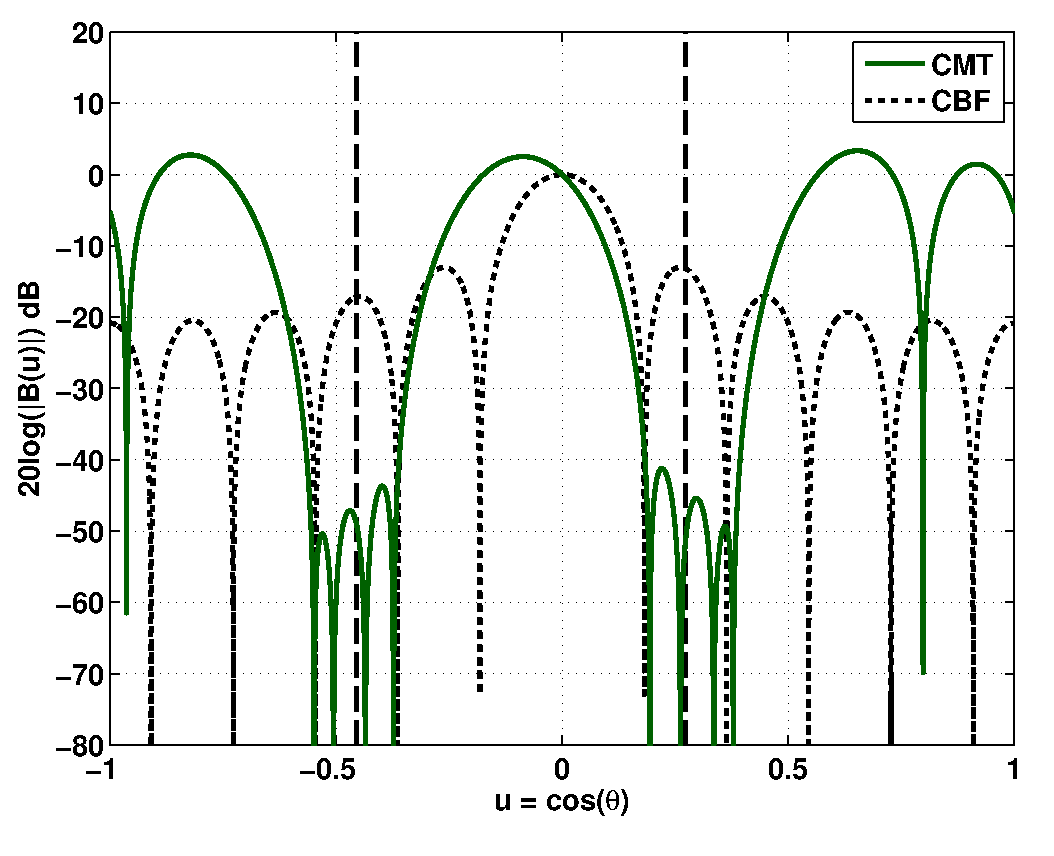
\includegraphics[width=0.5\textwidth]{cmt_bp.pdf}\label{fig:cmt-bp}}

  \subfloat[]{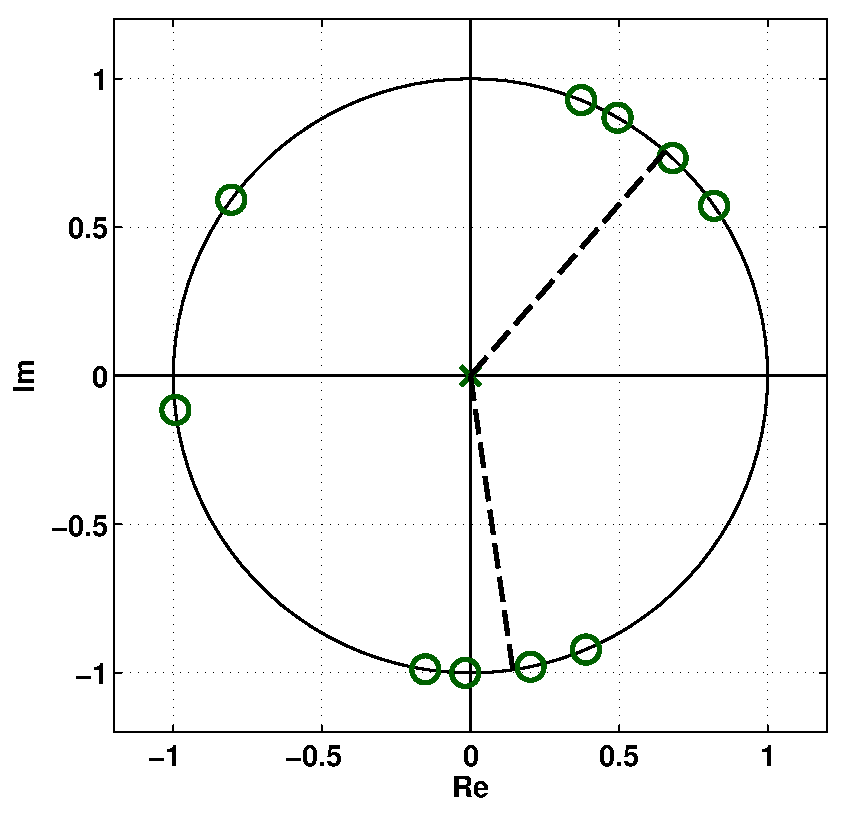
\includegraphics[width=0.5\textwidth]{cmt_pz.pdf}\label{fig:cmt-pz}}

  \caption{(a) Log-magnitude beampattern and (b) zeros of CMT MVDR ABF using $N = 11$ sensor ULA and steered towards $\ulook = 0$. The CMT notch width $\cmtW = 2/(N-1$). Two interferers are present at directions $\uinter = 3/N$ and $-5/N$ denoted by dashed vertical lines in (a) and dashed radial lines in (b). The CMT MVDR uses four zeros per interferer to create broad notch at the cost of high sidelobes and wider mainlobe.}
\label{fig:cmt-bp-pz}
\end{figure}

\figurename{}~\ref{fig:cmt-bp-pz} shows the log-magnitude beampattern
(top panel) and the polynomial zeros (bottom panel) of a CMT MVDR ABF
(solid green) implemented using $N = 11$ sensor ULA assuming the ECM
is known. A CBF beampattern (dotted black) is also shown for
reference. Two independent interferers are present at $\uinter = 3/N$
and $-5/N$ respectively as denoted by the vertical dashed lines in
beampattern and radial dashed lines in zeros plot. The CMT notch width
is set to $\cmtW = 2/(N-1)$. Examining the beampattern, the CMT MVDR
ABF produces broad notch at each interferer direction. The notch
broadening is achieved by clustering multiple beampattern nulls in the
vicinity of the interferer direction. Equivalently, the associated CMT
MVDR polynomial zeros cluster in the vicinity of a interferer
direction, as seen in the zeros plot. For a given interferer strength,
the number of zeros used to produce the notch broadening depends on
the notch width parameter $\cmtW$. The wider the notch width
required, more zeros per interferer are used to produce notch
broadening. In the \figurename{}~\ref{fig:cmt-pz}, the CMT MVDR ABF is
using four zeros per interferer to produce broad notches. However, as
seen in the beampattern the CMT MVDR ABF produces broad notches at the
cost of high sidelobes and wider mainlobe which reduces the WNG
[\sect{}~\ref{sec:wng}].

\subsubsection{CMT as spatial modulation}
\label{sec:cmt-as-spatial}

\srt{Added this section to discuss how eigenanalysis of taper matrix explains the usage of three DoF per interferer when $\cmtW = 2/(N-1)$.}

The CMT approach of augmenting the SCM with the taper matrix
$\taperMat$ in \eqref{eq:taper-mat} is equivalent to performing
spatial modulation of the observed snapshots. The spatial modulation
of the snapshot generates fictitious sources around the planewave
sources contained in the snapshot. The eigendecomposition of the taper
matrix is
$\taperMat = \sum_{n=1}^{N}\eval_n\taperevec_n\taperevec_n\herm$ where
$\taperevec_n$ is the $n\nth$ eigenvector and $\eval_n$ is the
associated eigenvalue such that
$\eval_1 \geq \eval_2 \geq \ldots \eval_N$. The number of significant
eigenvalues of the taper matrix in \eqref{eq:taper-mat} is
$\cmtW(N-1)/2 + 1$ \cite{song2003null}. Hence, for a notch width of
$W = 2/(N-1)$, the taper matrix $\taperMat$ has only two significant
eigenvalues. Using the eigendecomposition of $\taperMat$, the tapered
SCM is
\begin{align*}
  \sampCov_{T} &= \left( \frac{1}{L}\sum\limits_{\ell = 1}^{L}\datavec_{\ell}\datavec_{\ell}\herm \right) \circ \left( \sum\limits_{n=1}^{N}\eval_n\taperevec_n\taperevec_n\herm \right).\\
  \intertext{Considering only the two largest eigenvalues $\eval_1$ and $\eval_2$, and rearranging the terms,}
  \
   \sampCov_{T} &= \frac{1}{L}\sum\limits_{n=1}^{2}\eval_n\sum\limits_{\ell = 1}^{L}(\datavec_{\ell}\circ\taperevec_n)(\datavec_{\ell}\circ\taperevec_n)\herm\\
               &= \frac{1}{L}\sum\limits_{n=1}^{2}\eval_n\sum\limits_{\ell = 1}^{L}\modvec_{n\ell}\modvec_{n\ell}\herm \\
               &= \sum\limits_{n=1}^{2}\eval_n\sampCov_n
\end{align*}
where $\modvec_{n\ell} = (\datavec_{\ell}\circ\taperevec_n)$ is the
$\ell\nth$ snapshot modulated by $\taperevec_n$ and
$\sampCov_n$ is the SCM obtained by averaging the snapshots modulated
by $\taperevec_n$ for $n = 1, 2$. Hence, the tapered SCM
$\sampCov_{T}$ is a combination of $\sampCov_n$ weighted
by the eigenvalues ($\eval_n$) of the taper matrix.

\figurename{}~\ref{fig:cmt-eigenbeam} shows the magnitude of
eigenbeams of the first two principal eigenvectors $\taperevec_1$
(blue) and $\taperevec_2$ (green). The eigenbeam for $\taperevec_1$
has a single mainlobe in the broad side direction, identical to a CBF
beampattern steered to the broadside direction. This eigenbeam
indicates that snapshot modulation by $\taperevec_1$ keeps the
planewave signal in the snapshot, unchanged. However, the eigenbeam
for $\taperevec_2$ has two distinct peaks on either side of the
broadside direction. The two peaks in the eigenbeam indicates that
snapshot modulation by $\taperevec_2$ produces scaled copies of the
planewave signal in the snapshot, on either side of the signal
direction. In effect, the CMT operation using the taper matrix in
\eqref{eq:taper-mat} introduces a pair of fictitious sources on either
side of the interferer direction. Hence, an MVDR ABF implemented using
the tapered SCM $\sampCov_{T}$ places notch on either side of the
interferer direction, effectively producing broader notch as seen in
\figurename{}~\ref{fig:cmt-bp}. Consequently, the CMT MVDR ABF using
notch width $\cmtW = 2/(N-1)$ uses three degree of freedom (DoF) per
interferer to produce notch broadening.

\begin{figure}[!htb]
  \centering
  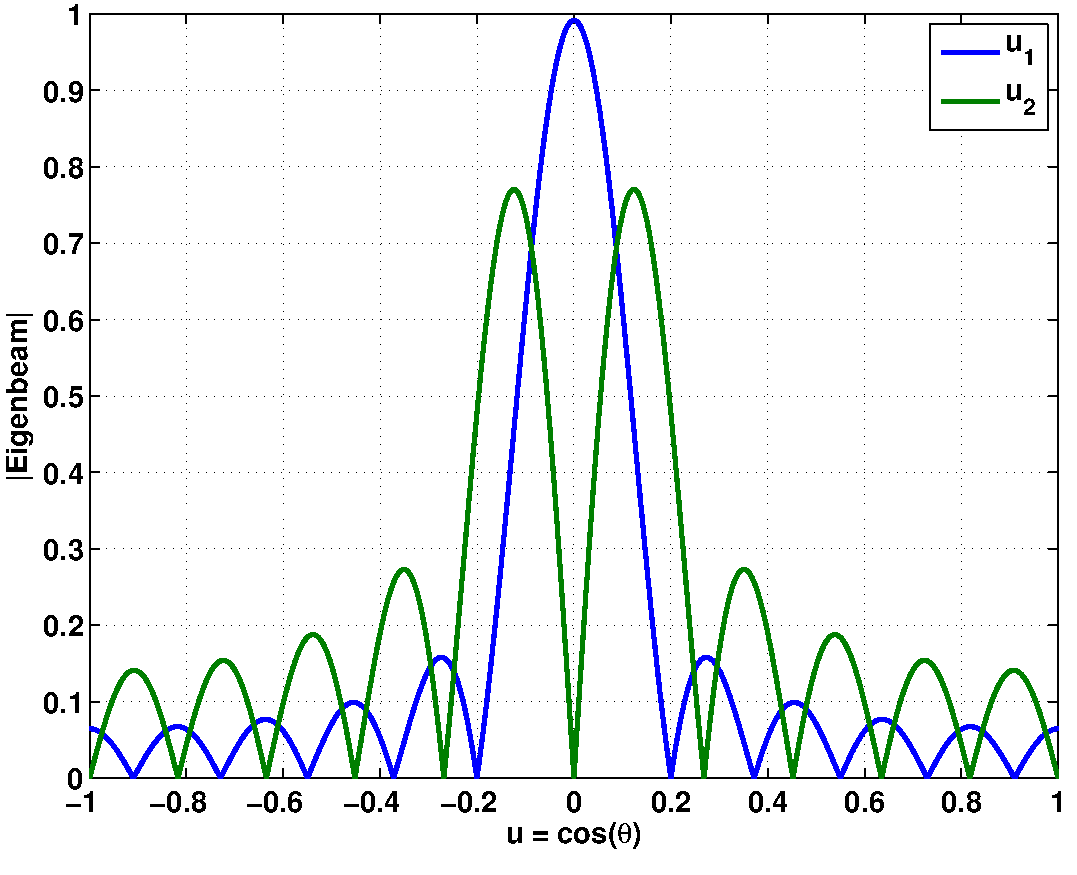
\includegraphics[width=0.8\textwidth]{cmt_eigval_beam.pdf}
  \caption{Magnitude of eigenbeam for first two principal eigenvectors of taper matrix in \eqn{}\eqref{eq:taper-mat}. The eigenvectors spatially modulate the snapshots to create replica of planewave signal in the snapshot on either side of the signal direction.}
  \label{fig:cmt-eigenbeam}
\end{figure}

\section{Properties of the beampattern near a  zero}
\label{sec:second-order-zeros}
Evaluating the array polynomial \eqref{eq:beampat-poly} on the unit
circle $z = e^{j\pi u}$ yields the beampattern in
\eqref{eq:beampatu}. The array polynomial $\beampolyz{}$ has $N - 1$
zeros in the complex plane and the zeros that fall on the unit circle
produce nulls in the beampattern. A first-order zero on the unit
circle produces a `sharp' null in the beampattern. The beampattern in
the neighborhood of a first-order null is linear in the directional
cosine $u$ \cite[Sec.~3.2.3]{vtree2002oap}\cite{Steinberg1976}. In contrast, the
second-order zeros (SOZ) produce flatter nulls in the beampattern. The
beampattern in the neighborhood of a second-order null is quadratic in
directional cosine $u$. \figurename{}~\ref{fig:mvdr-null-zero}
compares the MVDR beampattern magnitude in the neighborhood of a first-order
null (blue solid) and a second-order null (red dashed). The SOZ effectively
imposes a first derivative constraint on the beampattern which forces
the second-order null to be flatter compared to the sharp first-order
null.

As previously discussed, the ensemble MVDR beamformer places a
beampattern null in the neighborhood of the true interferer direction
to attenuate the interferer. The vertical dashed line in
\figurename{}~\ref{fig:mvdr-null-zero} denotes the interferer
direction $\uinter$. The interferer falls on the 'shoulder' of the
null where the first-order null creates a sharp notch whereas the
second-order null creates a deeper and broader notch. Any mismatch in
the interferer direction changes the ND at the interferer direction
$\uinter$. In case of a mismatch, the ND produced by the first-order
null exhibits greater variation compared to the second-order null
due to the linear and quadratic nature of their respective
beampatterns. As a result, the ND produced by the first-order null is
more sensitive to interferer direction mismatch compared to the ND
produced by the second-order null. The DZ MVDR ABF presented in the
next section exploits this property of a second-order null to produce
broader notches in the MVDR beampattern.

\begin{figure}[!hp]
  \centering
  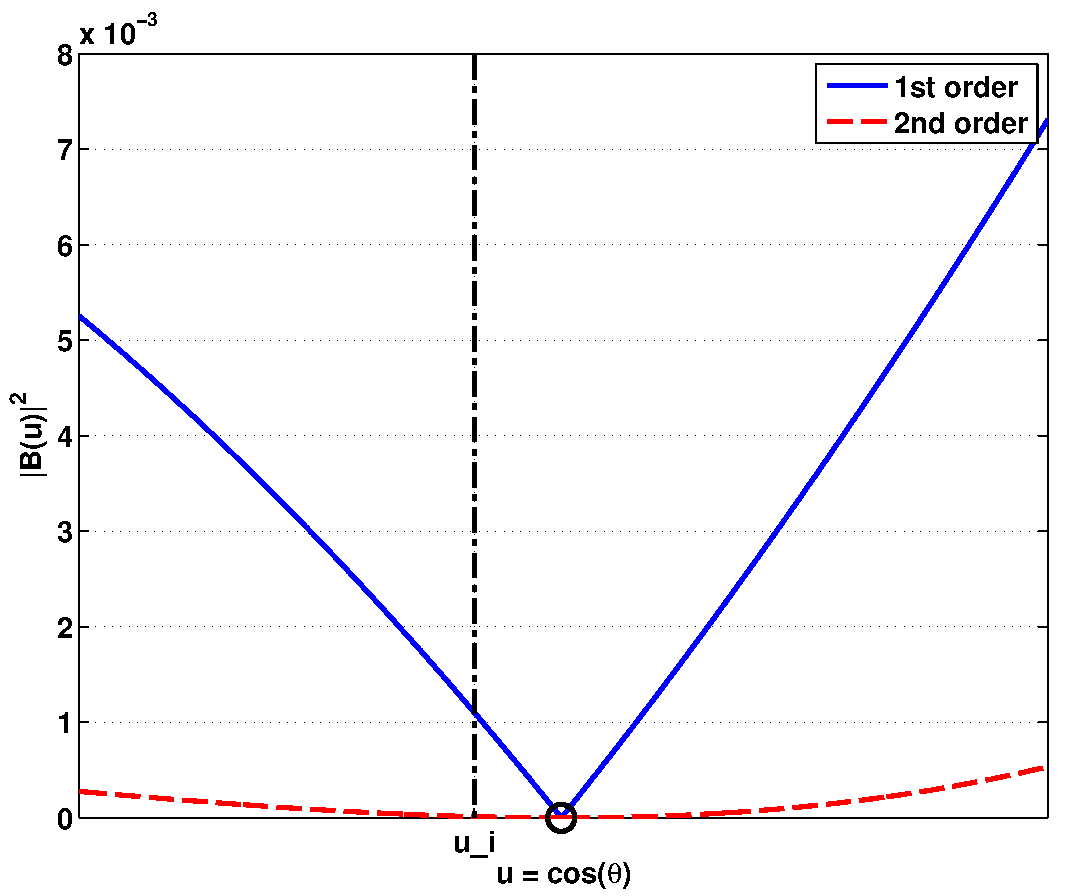
\includegraphics[width=0.8\textwidth]{interf_single_dbl_zero_beampattern.pdf}
  \caption{MVDR beampattern magnitude zoomed into the neighborhood of a
    null. The null location in directional cosine $u$ axis is denoted by
    the circle marker.  The vertical dashed line indicates the
    interferer direction. The blue solid curve denotes the first order
    null produced by the MVDR beamformer. The red dashed curve denotes
    a second order null in the same location.}
  \label{fig:mvdr-null-zero}
\end{figure}

% ==========================================
% Include files 

\section{Double Zero MVDR ABF}
\label{sec:double-zero-mvdr}
The double zero MVDR (DZ MVDR) ABF is designed to produce broad
beampattern notch in the interferer direction. The DZ MVDR algorithm
exploits the property of the SOZs of array polynomial to produce broad beampattern notches. The flow
diagram \figurename{}~\ref{fig:flow} provides an overview of the DZ
MVDR algorithm. The following section describes the DZ MVDR ABF
algorithm assuming the number of sensors $N$ is odd. The algorithm
extends naturally when $N$ is even by including an additional zero at
$u = 1$ as constrained by even symmetry even length array weights.

\subsection{Algorithm}
\label{sec:algorithm}
The DZ MVDR ABF begins with $L$ data snapshots from an $N$ element
ULA, represented as a data matrix $\dataMat{}$ of dimension
$N \times L$.  The data matrix $\dataMat{}$ is partitioned to create
two submatrices $\dataSubMat{{\rm a}} = \dataMat{(1:K, 1:L)}$ and
$\dataSubMat{\rm b} = \dataMat{(K:N, 1:L)}$ where $K = (N + 1)/2$. The
indices in the subscript of $\dataMat{}$ indicate the range of rows
and columns of $\dataMat{}$ assigned to each submatrix. This
partitioning of the data matrix is equivalent to partitioning the $N$
element full ULA into two $K$ element
subarrays shown in \figurename{}~\ref{fig:subarray}. The $(K-1)\nth$ sensor denoted by white circle is used in both subarrays. The submatrices $\dataSubMat{{\rm a}}$ and
$\dataSubMat{{\rm b}}$ are combined to create an augmented data matrix
$\dataMatK = [\dataSubMat{{\rm a}} | \dataSubMat{{\rm b}}]$ of
dimension $K \times 2L$. The data matrix $\dataMatK$ can be
interpreted as the collection of $2L$ snapshot observed by $K$ element
ULA.

The augmented data matrix is used to compute the subarray SCM
$\sampCov_{\rm K} = (\dataMatK\dataMatK\herm)/(2L)$ and subsequently
the ABF weight vector for a $K$ element subarray
\begin{equation}
  \label{eq:subarray-wt}
  \wtK = \frac{\sampCov_{K}\inv\rep_{K}}{(\rep_{K}\herm \sampCov_{K}\inv\rep_{K})}
\end{equation}
where $\rep_{K}$ is an array manifold vector in the look direction for
the $K$ element subarray. The beamformer in \eqref{eq:subarray-wt} can
be implemented as a SMI MVDR ABF on a $K$ element ULA. The DZ MVDR ABF
weight vector for the full ULA is obtained by convolving the weight vector
$\wtK$ with itself
\begin{equation}
  \label{eq:wt-convo}
  \wtdz = \wtK*\wtK
\end{equation}
where [*] denotes discrete convolution operation considering the weight vector
$\wtK$ as a discrete sequence of length $K$. The resulting DZ MVDR ABF
weight vector $\wtdz$ is of length $2K - 1 = N$.

 The z-transform of \eqref{eq:subarray-wt} yields the array polynomial of
 the subarray SMI MVDR ABF weight vector,
\begin{equation}
  \label{eq:subarray-poly}
  \beampolyz{{\rm K}} = \ztrans{(\wtK)} = G_K\prod_{i=1}^{K - 1}( 1 -
  \sampz_{Ki} z\inv).
\end{equation}
The array polynomial $\beampolyz{{\rm K}}$ has $(K - 1)$ first-order
zeros $\sampz_{Ki}$ on the complex plane. The convolution operation in
\eqref{eq:wt-convo} is equivalent to multiplying the array polynomial
$\beampolyz{{\rm K}}$ with itself to obtain the DZ MVDR array polynomial,
\begin{align*}
\beampolyz{{\rm DZ}} =& \beampolyz{{\rm K}}\beampolyz{{\rm K}} \\
                     =& G_K^2\prod\limits_{i=1}^{K - 1}( 1 -
                        \sampz_{Ki} z\inv)^2  = \ztrans{(\wtdz)}.
\end{align*}
Thus the convolution operation doubles the number of zeros from the
subarray SMI MVDR ABF to produce the DZ MVDR ABF. The DZ MVDR ABF
array polynomial $\beampolyz{{\rm DZ}}$ has $(K - 1)$ SOZs in the same
locations as $\sampz_{Ki}$  the zeros of the subarray SMI MVDR ABF.

The DZ MVDR ABF algorithm is extensible to the case when the number of
sensors $N$ is even. When $N$ is even, the subarray size is set to
$K = N/2$. In this case, the convolution operation produces only
$N - 2$ zeros in total while $N - 1$ zeros are required for a $N$
element ULA. The one additional polynomial zero required for the $N$
element ULA weight vector is chosen to be at $z = -1$. This choice is
motivated from the constraint that an FIR filter with a conjugate even
symmetric impulse response and odd number of zeros must have a zero at
$z = -1$ \cite[Sec.~5.7.3]{Oppenheim1989}.

% Algorithm block

\begin{algorithm}
  \caption{DZ MVDR beamformer} \label{alg:dzmvdr}
  \begin{algorithmic}
    \Procedure{SubarrayDataMatrix}{$\dataMat{}$}\Comment{Partition data
    matrix.}
     \State $\dataSubMat{{\rm a}} = \dataMat{1:K,1:L}$
     \State $\dataSubMat{{\rm b}} = \dataMat{K:N,1:L}$
     \State $\dataMatK = \dataSubMat{{\rm a}} | \dataSubMat{{\rm b}}$
    \EndProcedure
    \Procedure{MVDR}{$\dataMatK$}\Comment{Subarray SMI MVDR weights}
    \State $\sampCov_{K} = (\dataMatK \dataMatK\herm)/(2L)$
    \State  $\wtK = \sampCov_{K}\inv\rep_{K}/(\rep_{K}\herm \sampCov_{K}\inv\rep_{K})$
    \EndProcedure
    \Procedure{ConvolveWeights}{$\wtK$}
    \State $\wtdz = \wtK*\wtK$
    \EndProcedure
  \end{algorithmic}
\end{algorithm}


% ------ Flow diagram and sub-array configuration ------
\begin{figure}[!ht]
  \centering

  \subfloat[]
  {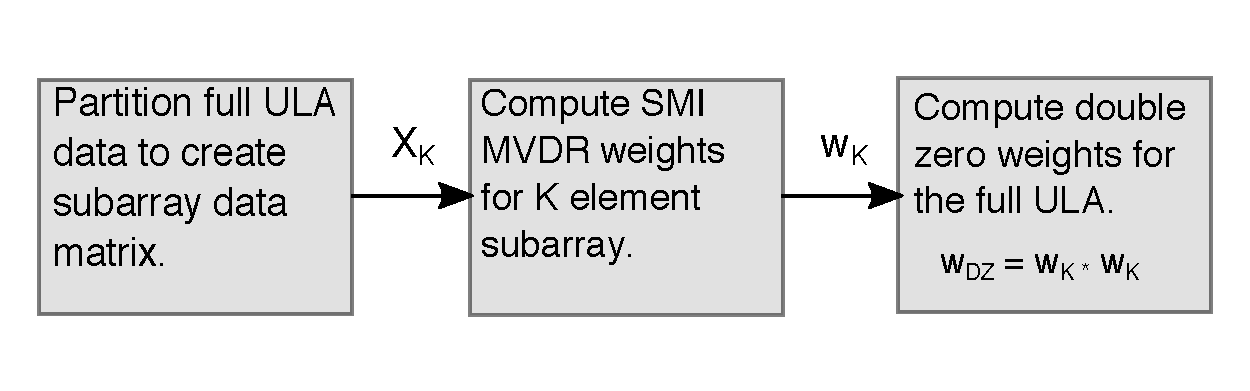
\includegraphics[width=5in]{dz_mvdr_flow.pdf}%
    \label{fig:flow}}
  \vfil

  \subfloat[] 
  {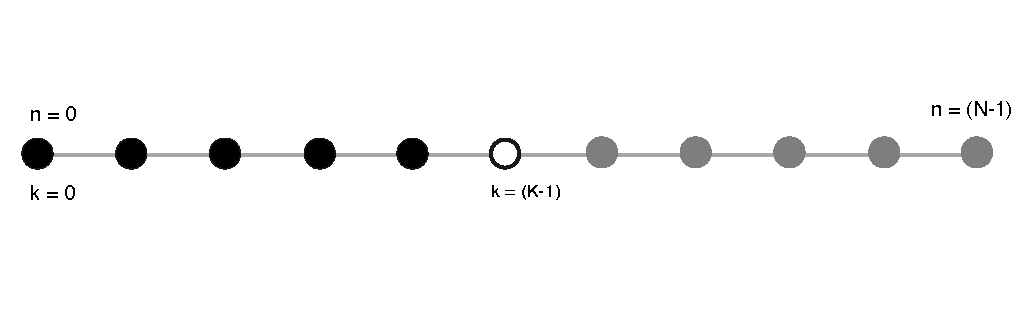
\includegraphics[width=5in]{sub_array.pdf}%
    \label{fig:subarray}}

  \caption{DZ MVDR algorithm (a) flow diagram and (b) two $K$ element
    subarray configuration within the $N$ sensor ULA.}
  \label{fig:dzmvdr}
\end{figure}
% ------------------------------------------------------

The DZ MVDR algorithm involves subarray processing using a $K$ element
subarray. Abraham and Owsley present subarray processing as a
technique to reduce computational overhead for ABFs implemented using
long arrays \cite{abraham89preproc}. The inherent subarray processing
in DZ MVDR ABF also reduces the computational requirement compared to the
standard SMI MVDR ABF implemented on a full ULA saving a factor of 8
in the computation of the SCM inverse. The SCM inversion operation in
\eqref{eq:subarray-wt} takes $\bigO{K^3}$ in contrast to $\bigO{N^3}$
required for the full ULA implementation. Further, the additional
convolution operation in \eqref{eq:wt-convo} takes no more than
$\bigO{K \operatorname{log} K}$. Further, the subarray SCM
($\sampCov_{\rm K}$) is computed using the augmented data matrix with
$2L$ subarray snapshots. The subarray SCM effectively has four times
more snapshots per sensor compared to the standard SCM computed using
the full ULA snapshots. The increase in snapshots to sensor ratio
lowers the bias in the subarray SCM eigenvector estimates which reduces
interferer mismatch \cite{benaych2011eigen, paul2007asymptotics}. The reduction in interferer mismatch enables the DZ MVDR ABF to place deeper notch at the interferer compared to the standard SMI MVDR ABF. 

The computation gain from subarray processing comes at the cost of
reduced spatial degree of freedom (DOF) and widening of the main-lobe
for the DZ MVDR ABF \cite{abraham89preproc}. The DOF is constrained to
about $N/2$, which limits the DZ MVDR ABFs ability to suppress
multiple interferers. Also, the use of $K$ element subarray produces a
main-lobe twice as wide compared to the SMI MVDR ABF using full ULA. A wider main-lobe implies reduced ability of the ABF to resolve two planewaves.

\subsection{Unit circle constrained DZ MVDR ABF}
\label{sec:unit-circle-constr}
As previously seen in Ch.~\ref{ch:mvdr}, the ensemble MVDR beamformer
polynomial zero locations are constrained on the unit circle for
planewave beamforming using a ULA. The DZ MVDR algorithm described
above can be modified to force all the SOZs onto the unit circle
thereby satisfying the unit circle constraint on ensemble case
zeros. In \eqref{eq:subarray-wt}, computing the subarray weights
$\wtK$ as a unit circle (UC) MVDR ABF weights instead of the SMI MVDR
weights produces $K - 1$ zeros $\sampz_{Ki}$ on the unit circle
\cite{tuladhar2015ucmvdr}. The DZ MVDR ABF weight vector $\wtdz$
derived by convolving the subarray UC MVDR weight vector $\wtK$ has
all the SOZs on the unit circle. The unit circle SOZs produce flatter
beampattern nulls and create broader notches in the interferer
direction as discussed in \ref{sec:array-poly-rep}. However enforcing
the UC constraint comes at a cost of additional computational overhead
of solving for the zeros of $K\nth$ order array polynomial to compute
the subarray UC MVDR ABF weights \cite{tuladhar2015ucmvdr}.

% \subsection{Higher-order-zero MVDR }
% \label{sec:higher-order-zero}
% Extending DZ MVDR to higher-order zero implementation for wider nulls.


%%% Local Variables:
%%% mode: latex
%%% TeX-master: "main"
%%% End:
  % algorithm description
\section{Simulation Results}
\label{sec:results}
This section discusses the results of the numerical experiments
evaluating the performance of the DZ MVDR ABF. The experiments are
conducted for two cases: (1) stationary interferers and (2) a moving
interferer. In the stationary interferer cases, the DZ MVDR ABF is
compared with the SMI MVDR and the DL MVDR ABFs. In the moving
interferer case, the DZ MVDR ABF is compared with the CMT MVDR ABF.
In the experiments, all ABFs are implemented using an $N = 31$ element
standard ULA and steered to broadside ($\ulook = 0$). The experiments
assume a passive sonar application where ABFs commonly operate with
barely sufficient snapshots $L = N + 1$ and even $L = 2N$ snapshots
is a relatively snapshot rich case
\cite{cox2002adaptive,baggeroer1999passive}. For all experiments, the
simulated snapshots consists of interferers and unit power white
background noise. No source signal is present in the simulated
snapshot data. All results discussed below are obtained from 3000
trials Monte Carlo experiment.

\subsection{Stationary interferer case}
\label{sec:stat-interf}
Stationary interferers maintain a fixed direction during the snapshot
averaging interval. Two scenarios with stationary interferers are
considered for evaluation of the ABFs. The first scenario has a single
narrowband interferer present at direction $\uinter = 3/N$ with $40$
dB of INR. The second scenario has four discrete narrowband
interferers at directions $\uinter = \{-7/N, ~-3/N, ~3/N, ~7/N \}$
with $\{30, ~20, ~20, ~30 \}$ dB of INR respectively.

\figurename{}~\ref{fig:pout-ecdf} shows the empirical cumulative
distribution function (ECDF) of the output power from the DZ MVDR ABF
compared with the SMI MVDR, and the DL MVDR ABFs. The left panels show
the ECDF graphs for the snapshot limited case ($L = 32$) and the right
panels show the ECDF graphs for the snapshot sufficient case
($L = 62$). The dotted vertical line in each panel denotes the
ensemble output power ($P_{\rm ens}$) produced by the MVDR beamformer
implemented using the knowledge of the ECM. The ensemble output power
is the ideally possible minimum output power for the experimental
scenario. The output power level corresponding to the ECDF value of
$0.5$ denotes the median output power. The closer the median is to the
dotted vertical line, higher the probability of the ABFs to produce
output power comparable to the ensemble output power. The DL factor
for the DL MVDR ABF is set to match the average WNG between the DL
MVDR ABF and the DZ MVDR ABF in each case.

In all four cases in \figurename{}~\ref{fig:pout-ecdf} the DZ MVDR ABF
exhibits higher probability of producing lower output power compared
to the SMI MVDR and the DL MVDR ABF, over the observed output power
range. When snapshot limited ($L = 32$), the DZ MVDR median output
power is less than the SMI MVDR ABF median output power by a factor of
ten. When snapshot sufficient ($L = 62$) the DZ MVDR median output
power is less than the SMI MVDR ABF median output power approximately
by a factor of $1.5$. The DZ MVDR ABF exhibits the greatest
improvement over the SMI MVDR ABF in the snapshot limited
cases. Moreover, the DZ MVDR ABF achieves consistently lower median
output power independent of the snapshots for both single and multiple
interferer scenarios. In contrast, the SMI MVDR ABF's output is
sensitive to the number of snapshots available.

For all interferer scenarios and snapshot conditions, the ECDF of the
DZ MVDR ABF is comparable with the DL MVDR ABF which has the same average
WNG. Examining the snapshot limited ($L = 32$) case for both single
and multiple interferer scenario the DZ MVDR ABF has lower median
output power than the DL MVDR ABF. The lower output power indicates that
the DZ MVDR ABF suppresses the interferer and noise better than the DL
MVDR ABF. In the snapshot sufficient ($L = 62$) case for both single
and multiple interferer scenario, the DZ MVDR and the DL MVDR ABF have
essentially equal median output power. However the DL MVDR ABF
requires a prior choice of the DL factor whereas the DZ MVDR ABF
achieves same performance without the need to choose a design
parameter.

\begin{figure*}[!hp]
  \centering
  \subfloat[Single interferer, L = 32]  {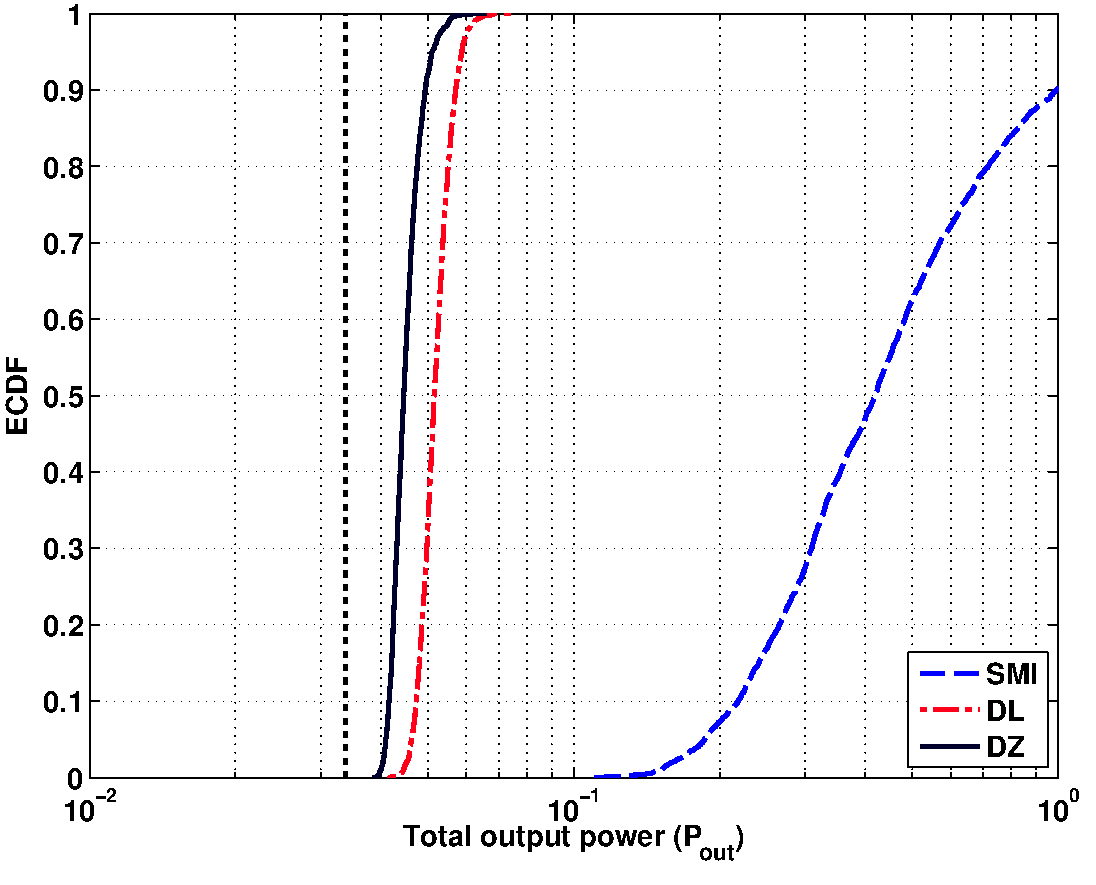
\includegraphics[width=3in]{total_pout_ecdf_single_interf_N31_L32_INR40.pdf}%
    \label{fig:pout-s-L32}}
\subfloat[Single interferer, L = 62]
{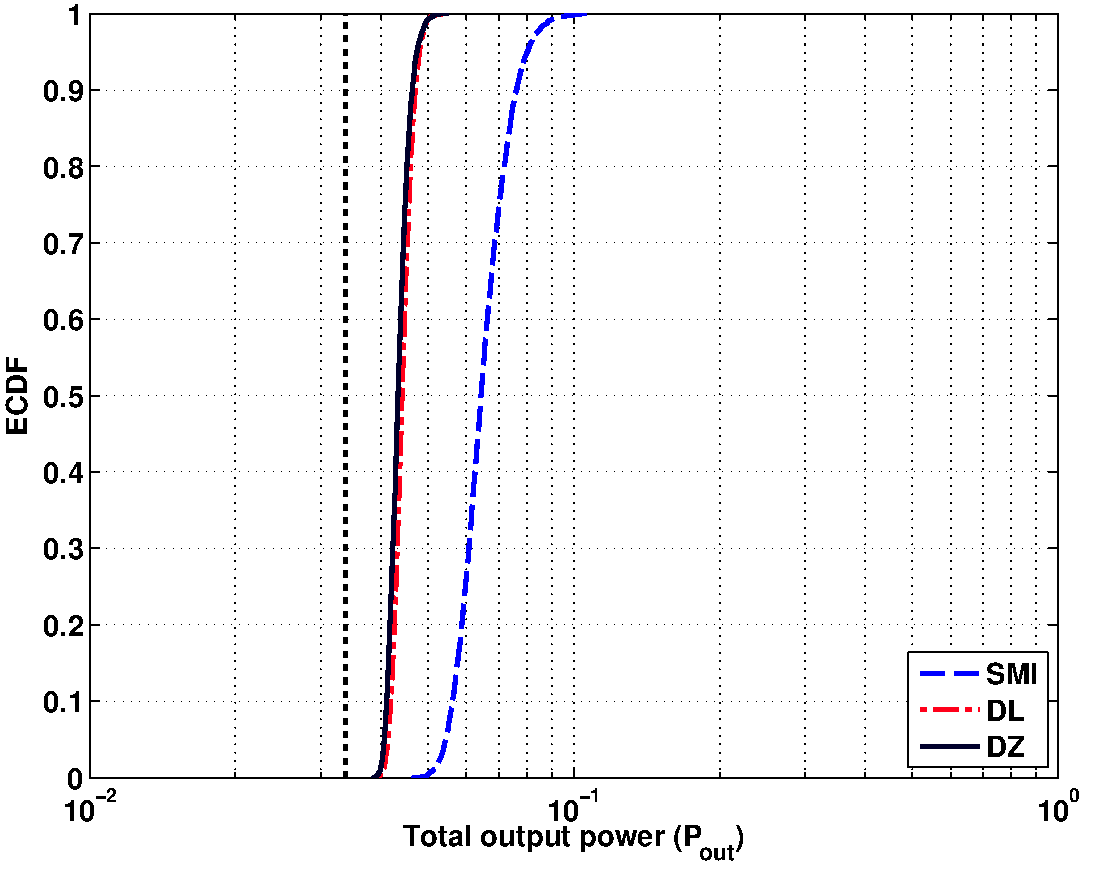
\includegraphics[width=3in]{total_pout_ecdf_single_interf_N31_L62_INR40.pdf}%
    \label{fig:pout-s-L62}}

  \subfloat[Multiple interferers, L = 32]
  {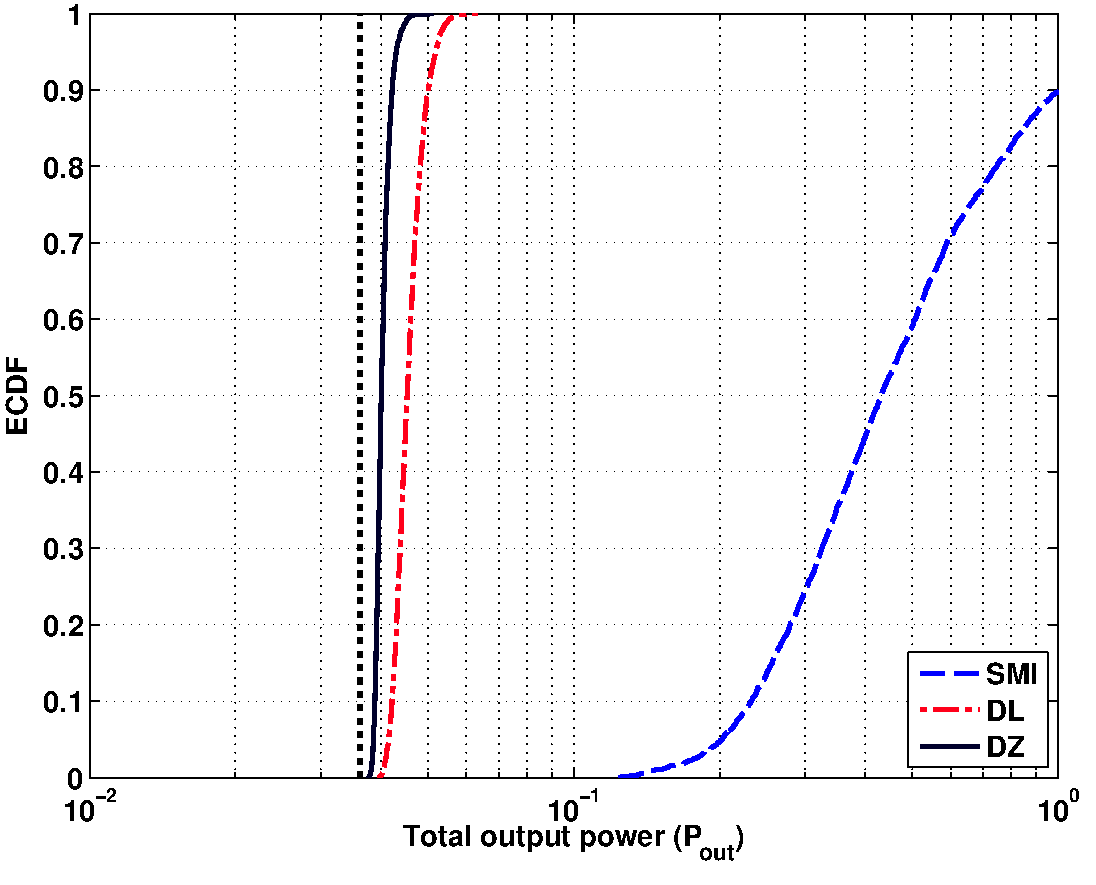
\includegraphics[width=3in]{total_pout_ecdf_multi_interf_N31_L32.pdf}%
    \label{fig:pout-m-L32}}
  \subfloat[Multiple interferers, L = 62]
  {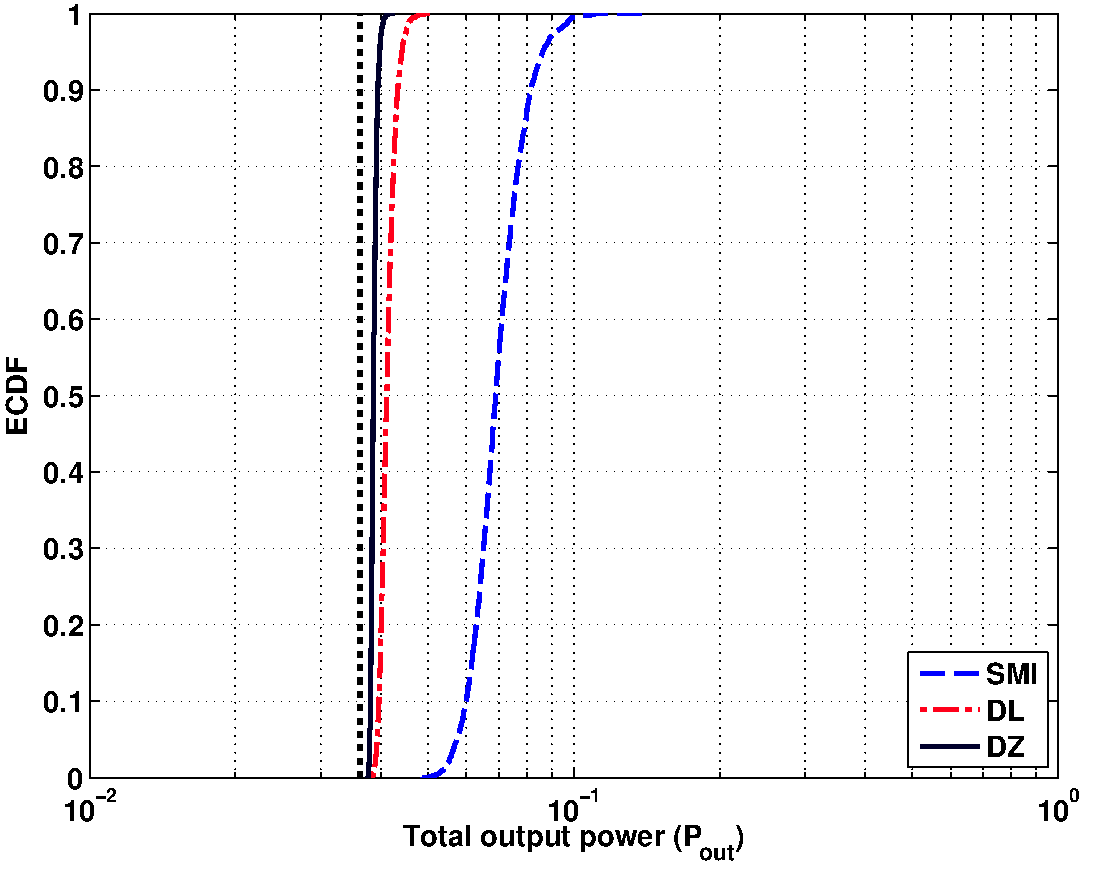
\includegraphics[width=3in]{total_pout_ecdf_multi_interf_N31_L62.pdf}%
    \label{fig:pout-m-L62}}
  \caption{Output power ECDF for the SMI MVDR, DL MVDR and the DZ MVDR
    ABFs using an $N = 31$ element ULA. The vertical dotted line
    denotes the ensemble MVDR output power level. The DZ MVDR ABF has
    higher probability of producing lower output power than the SMI
    MVDR and the DL MVDR ABFs.}
  \label{fig:pout-ecdf}
\end{figure*}

\figurename{}~\ref{fig:ecdf-dz-dzuc} compares output power of the DZ
MVDR ABF and the UC constrained DZ MVDR ABF. The left panel shows the
single interferer scenario while the right panel shows the multiple
interferers scenario in a snapshot limited case ($L = 32$). Comparison
shows that in both scenarios, the DZ MVDR and the UC constrained DZ
MVDR have essentially the same ECDF. The UC constraint yields only a
minimal improvement over the DZ MVDR ABF. Thus, zero doubling in the
DZ MVDR ABF is contributing to most of the gain over SMI MVDR
ABF. Moreover implementing the UC constrained DZ MVDR ABF only
introduces computational overhead as discussed in
Sec.~\ref{sec:unit-circle-constr}. Hence UC constrained DZ MVDR ABF
does not improve performance sufficiently to justify the additional
computational cost of solving for the roots of the $K = 16\nth$ order
array polynomial required for combining the UC and the DZ
algorithms. Also in both interferer scenarios, the DZ MVDR ABF has
lower median output power compared to the standard UC MVDR ABF for a
far smaller computational cost \cite{tuladhar2015ucmvdr}.

\begin{figure}[!ht]
\centering
\subfloat[Single interferer]{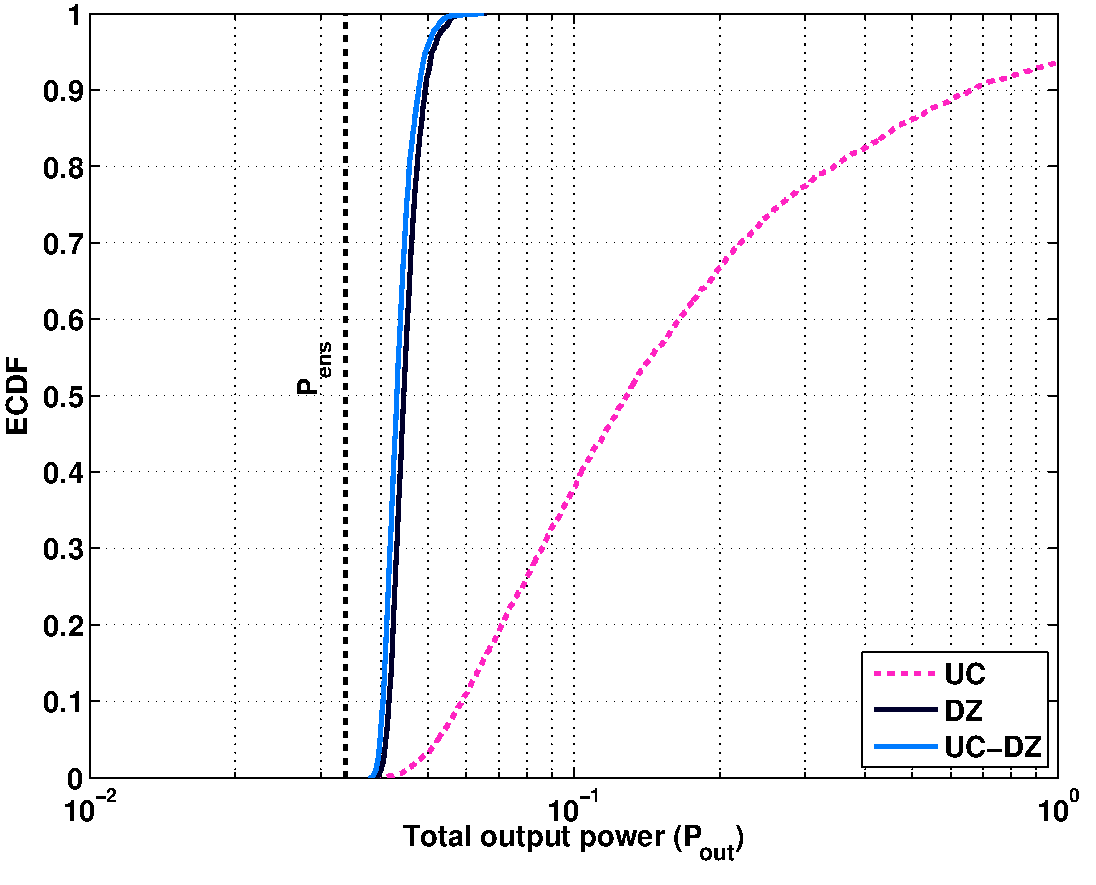
\includegraphics[width=3in]{dz_ucdz_ecdf_comp_single_interf.pdf}}
\subfloat[Multiple interferers]{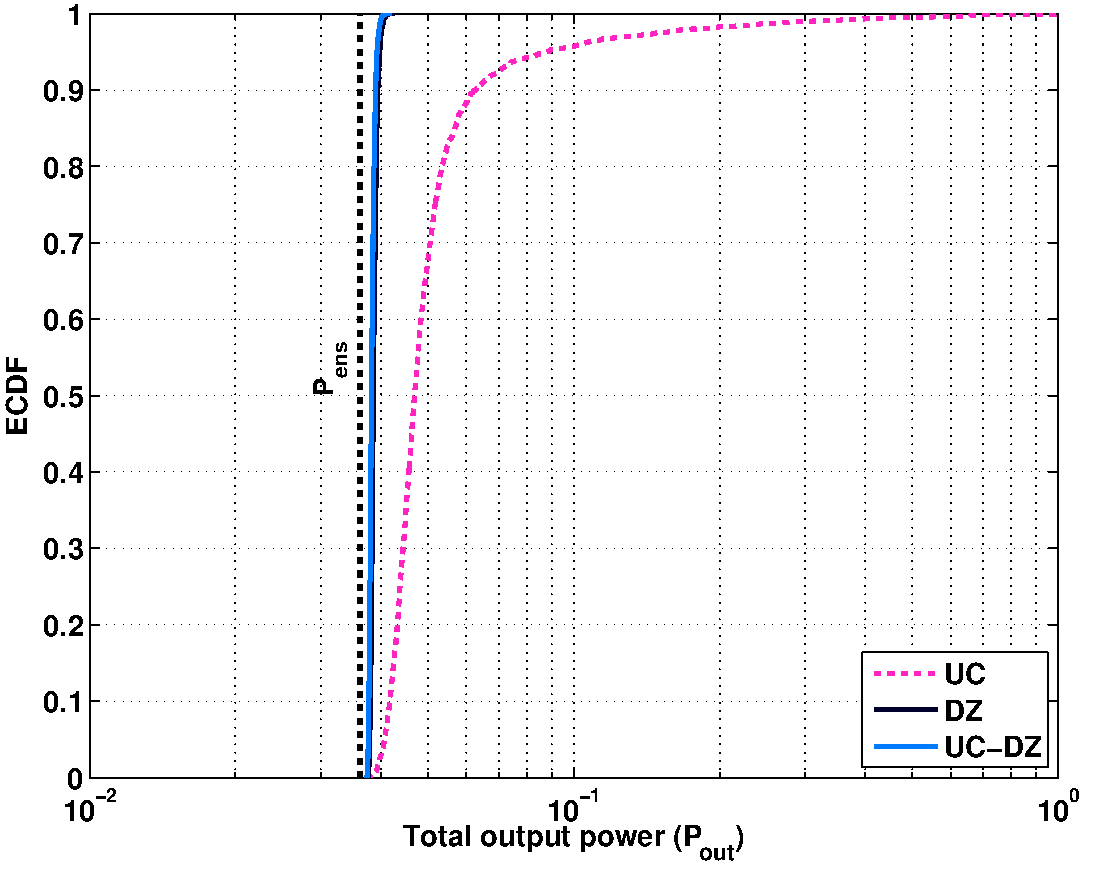
\includegraphics[width=3in]{dz_ucdz_ecdf_comp_multi_interf.pdf}}

\caption{Output power ECDF for the DZ MVDR, the unit circle (UC)
  constrained DZ MVDR and the UC MVDR ABFs using an $N = 31$ element ULA
  and $L = 32$ snapshots. The UC constraint yields only a minimal gain
  over the DZ MVDR ABF.}
\label{fig:ecdf-dz-dzuc}
\end{figure}

% Multi interferer case: dz_ucdz_ecdf_comp_multi_interf

% THIS CAN GO INTO DISSERTATION
% % Mean var result discussion
% \figurename{}~\ref{fig:pout-mean-var-plots} compares the mean (solid) and
% variance (dashed) of the output power for the SMI MVDR ABF and the DZ MVDR
% ABF for the single interferer scenario, over a range of input INR levels
% from $0$ dB to $40$ dB. The DZ MVDR ABF produces output power with both lower
% mean and lower variance compared to the SMI MVDR ABF. The reduced mean output
% power demonstrates the DZ MVDR ABF's ability to suppress
% interferers. The reduced variance on output power suggests the DZ MVDR
% beamformer should achieve better detection performance as well.

% % Mean and var figure
% \begin{figure*}[!t]
%   \centering
%   \subfloat[$L = 32$]
%   {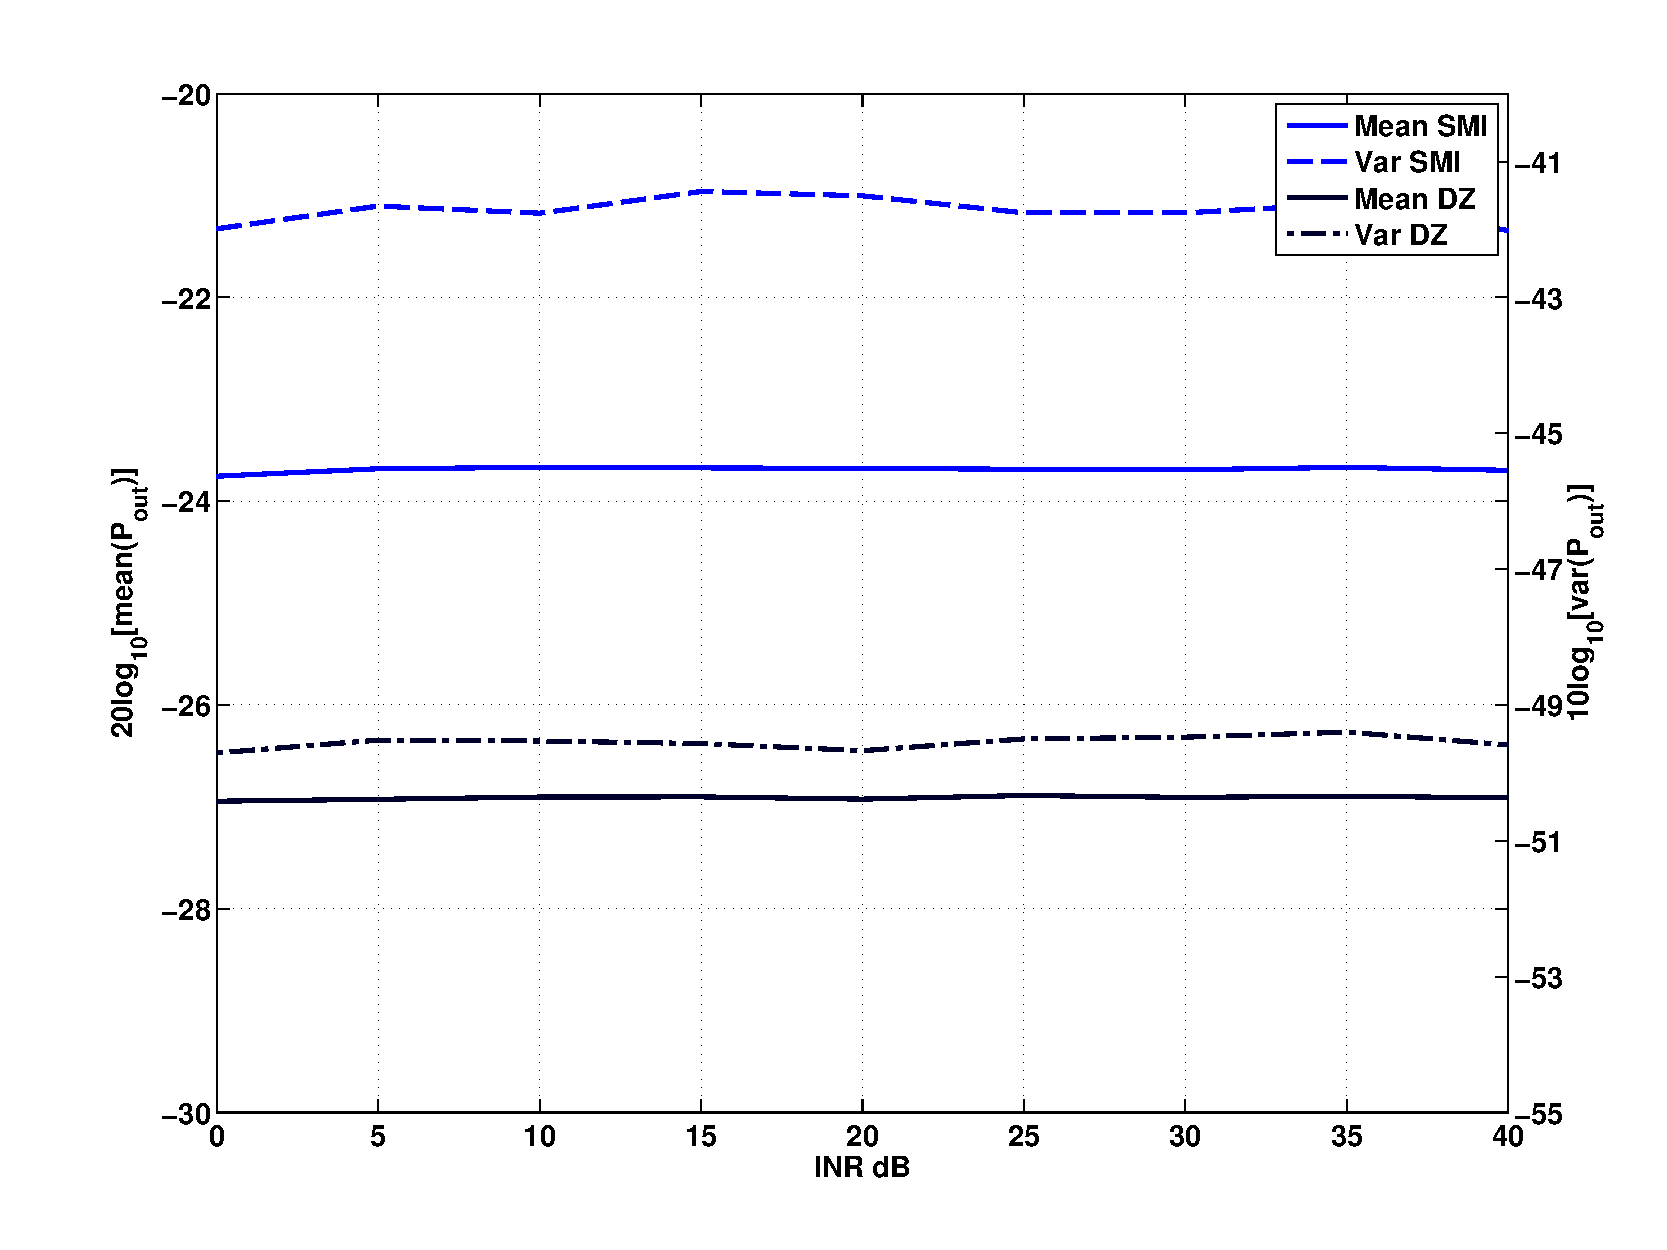
\includegraphics[width=2.8in]{mean_var_Pout_single_interf_N31_L62.pdf}
%     \label{fig:mean-var-single}}
%   \hfil
%   \subfloat[$L = 62$]
%   {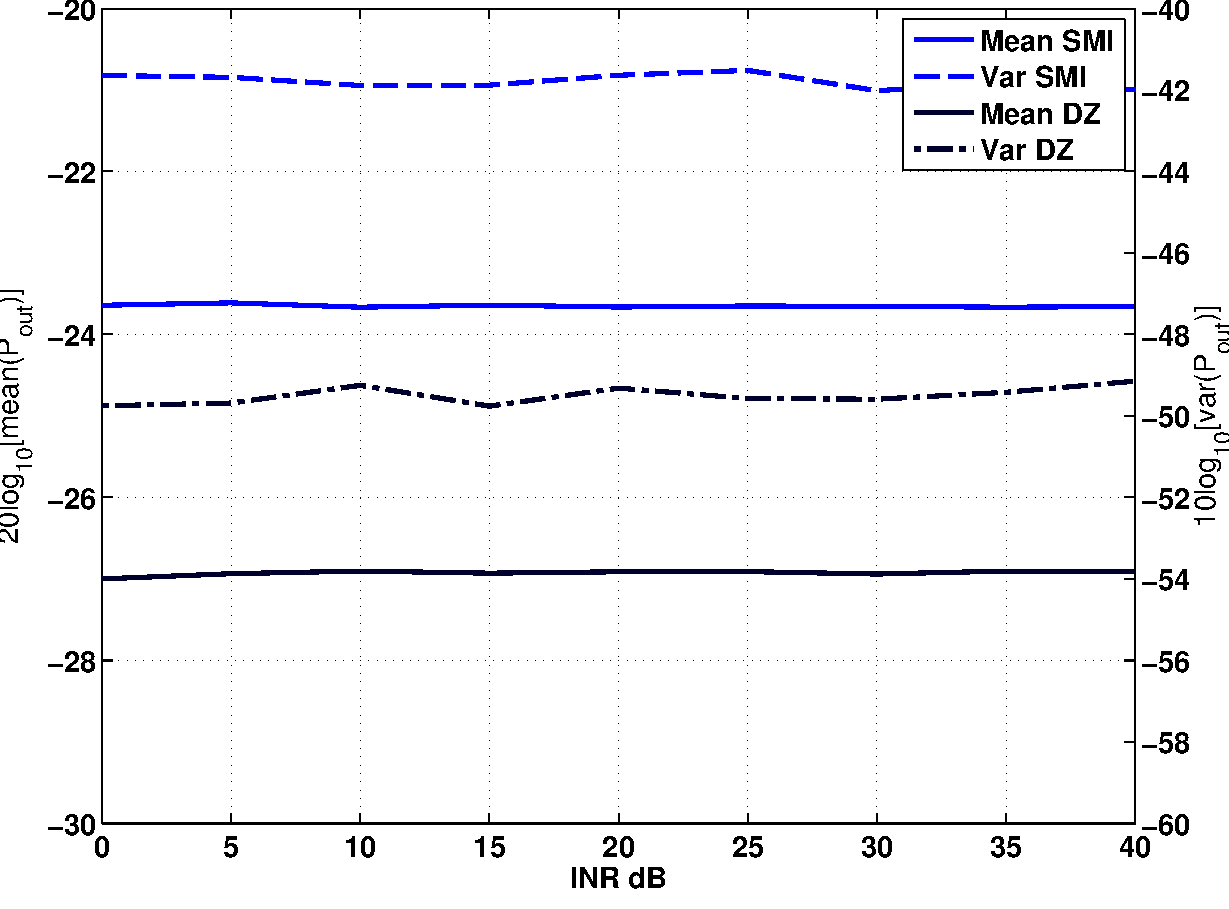
\includegraphics[width=2.8in]{mean_var_Pout_multi_interf_N31_L62.pdf}
%     \label{fig:mean-var-multi}}
%   \caption{Mean and variance of ABF output power over a range of input
%     INR for single interferer case. The DZ MVDR ABF output power has both lower mean and variance
%     compared to the SMI MVDR ABF.}
%   \label{fig:pout-mean-var-plots}
% \end{figure*}

% WNG discussion
\figurename{}~\ref{fig:wng-scatter} shows a scatter plot of the WNG
for the DZ MVDR and the SMI MVDR ABF. The top panel shows single
interferer scenario and the bottom panel shows the multiple interferer
scenario. In both plots, dot markers denote the snapshot limited case
($L = 32$) and the asterisk markers denote the snapshot sufficient
case ($L = 62$). Each dot and asterisk plots the WNG of the DZ MVDR
ABF against the WNG of the SMI MVDR ABF for one realization in the
Monte Carlo experiment. The optimal WNG for the experiment is $N = 31$
and the top right corner of the panel corresponds to the optimal WNG
for both ABFs \cite{vtree2002oap}. For all interferer scenarios and
snapshot conditions examined, the DZ MVDR ABF has better WNG than the
SMI MVDR ABF for almost every experimental trial. The DZ MVDR ABF
achieves consistently high WNG independent of the number of snapshots
for both the single and multiple interferer scenarios. In contrast,
the SMI MVDR ABF's WNG is very sensitive to the number of snapshots
available.  From the scatter plots, the DZ MVDR ABF exhibits higher
WNG on average compared to the SMI MVDR ABF. In addition to improving
the DZ MVDR ABF's ability to reject white background noise, the
improved WNG also indicates improved robustness against parameter
mismatch \cite{Gilbert1955}.

\begin{figure*}[!hp]
\centering
\subfloat[Single interferer]{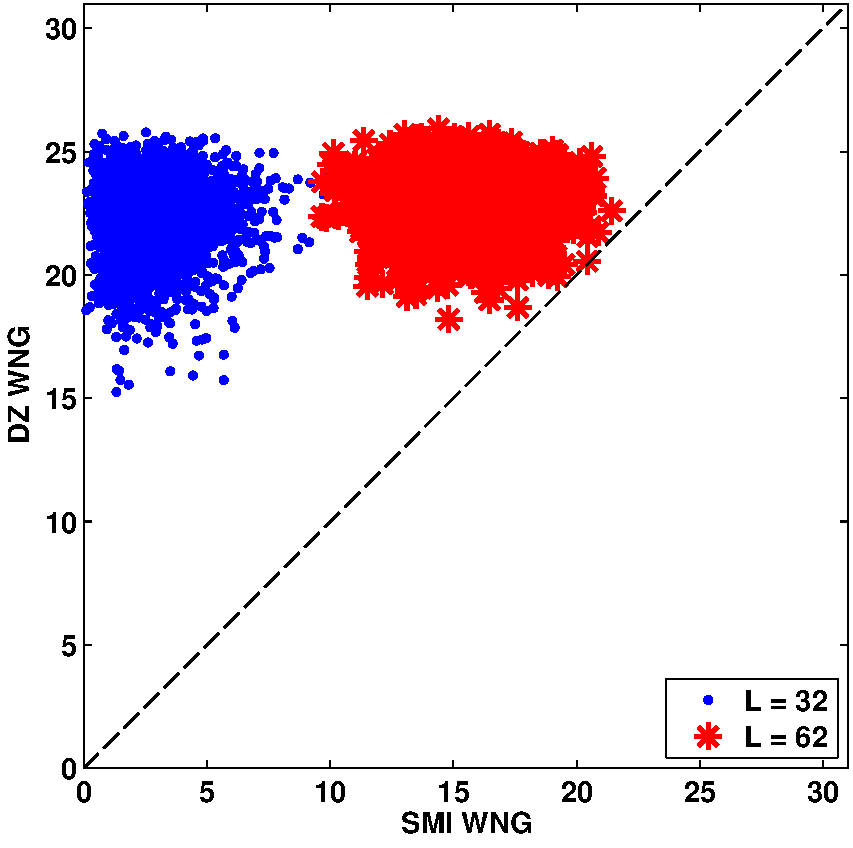
\includegraphics[width=3in]{wng_scatter_composite_single_N31.pdf}
%\subfloat[L = 32]{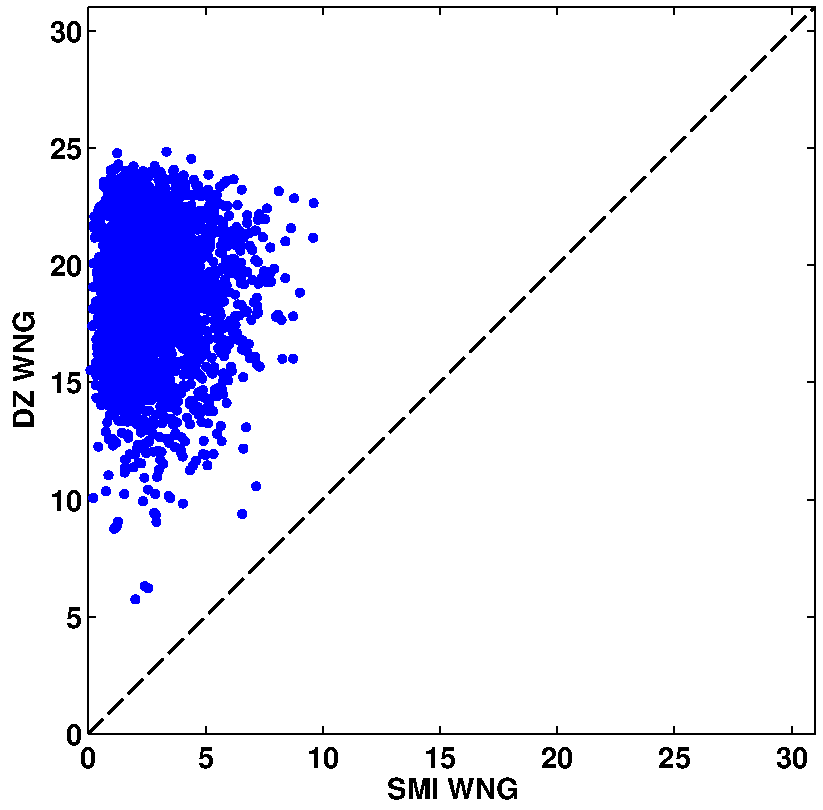
\includegraphics[width=2.5in]{wng_single_interf_N31_L32_INR40.pdf}
\label{fig:wng-s-L32}}

\subfloat[Multiple interferer]{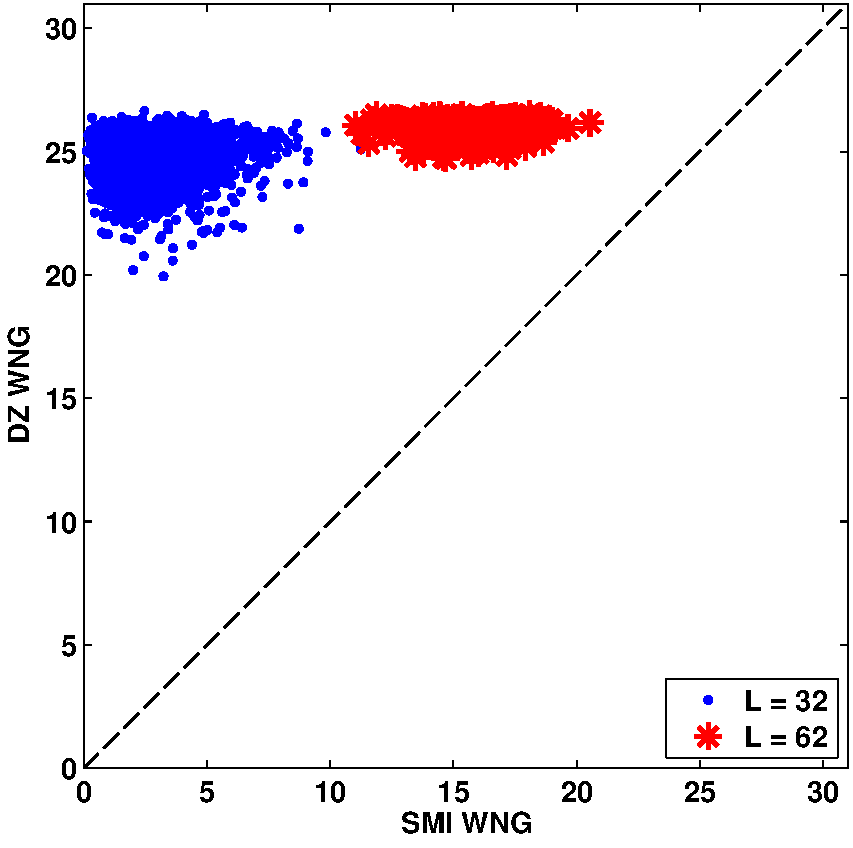
\includegraphics[width=3in]{wng_scatter_composite_multi_N31.pdf}
%\subfloat[L = 62]{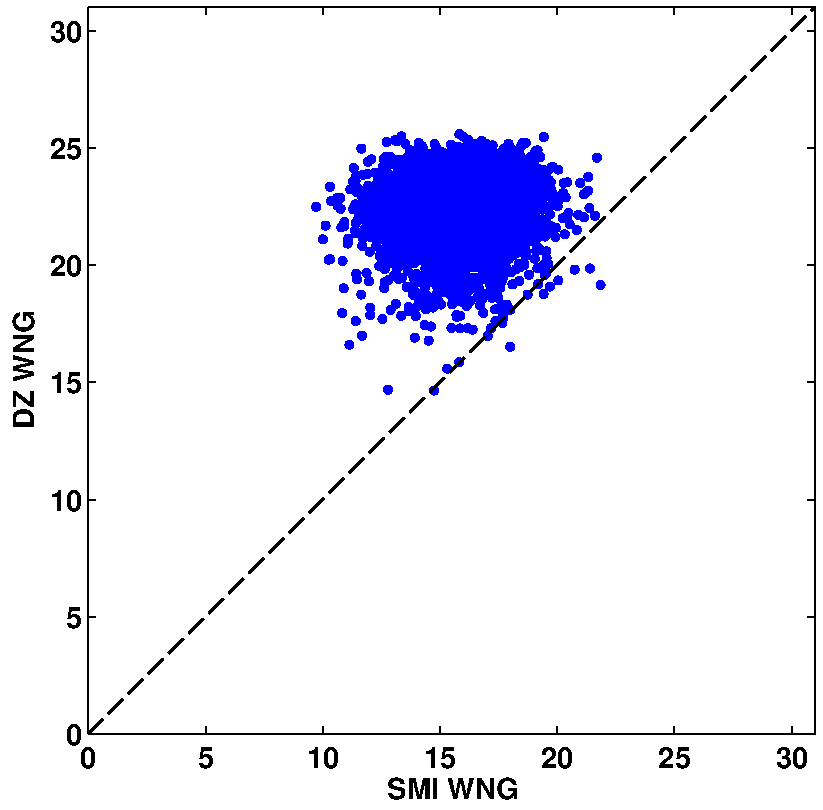
\includegraphics[width=2.5in]{wng_single_interf_N31_L62_INR40.pdf}
\label{fig:wng-s-L62}}
\caption{WNG scatter plot comparing the DZ MVDR and the SMI MVDR ABFs
  using an $N = 31$ element ULA. On average, the DZ MVDR ABF has a
  higher WNG.}
\label{fig:wng-scatter}
\end{figure*}

% Output vs snapshot
\figurename{}~\ref{fig:pout-snapshot} compares the mean output power
between the DZ MVDR, the SMI MVDR, and the DL MVDR ABFs for
implementations using $L = [32, 48, 62]$ snapshots. The top panel
shows the single interferer scenario and the bottom panel shows the
multiple interferer scenario. In both panels, the solid horizontal
line denotes the ensemble MVDR output power. For both interferer
scenarios and all snapshot cases, comparisons show that the DZ MVDR ABF
produces consistently lower mean output power compared to the SMI MVDR
ABF. When snapshot rich ($L = 62$), the DZ MVDR ABF output power is
lower than the SMI MVDR ABF output only by a factor less than two in
both the single and the multiple interferer scenarios. But when
snapshot limited ($L = 32$) the DZ MVDR ABF mean output power is lower
than the SMI MVDR ABF mean output power by a factor more than ten. As
mentioned previously, the decrease in the number of snapshots results
in an increased interferer direction mismatch. The mismatch leads to the
loss of interferer suppression for the SMI MVDR ABF and produces
higher output power. At the same time, the DZ MVDR ABF with its
broader notches is robust against the interferer direction
mismatch. The broader notches consistently suppress the interferers to
produce lower mean output power compared to the SMI MVDR ABF.

In the experiment, for both interferer scenarios and each snapshot
case, the DL factor for the DL MVDR ABF is chosen to match the average
WNG between the DL MVDR and the DZ MVDR ABFs. Hence the two ABFs have
comparable white noise power suppression. In
\figurename{}~\ref{fig:pout-snapshot}, comparisons between the DZ MVDR
and the DL MVDR ABFs shows that they have essentially same output
power performance for all cases in both interferer scenarios. This
implies that the output power is dominated by white noise contribution
and the interferer power contribution is negligible. Both the DZ MVDR
and the DL MVDR ABFs suppress the interferer power significantly
better compared to the SMI MVDR ABF. However, the approach used to
choose WNG in the experiment is not realistic as it requires
iteratively solving for the DL factor to match the average WNGs. In
practice the DL MVDR ABF still requires choosing a DL factor, while
the DZ MVDR ABF does not require setting a design parameter prior to
implementation. On the other hand, the DL MVDR ABF can in principle
handle more than $N/2$ interferers, while the DZ MVDR ABF is limited
to to about $N/2$ interferers due to the subarray approach
constraining the number of degrees of freedom.

\begin{figure*}[!hp]
\centering
\subfloat[Single interferer]{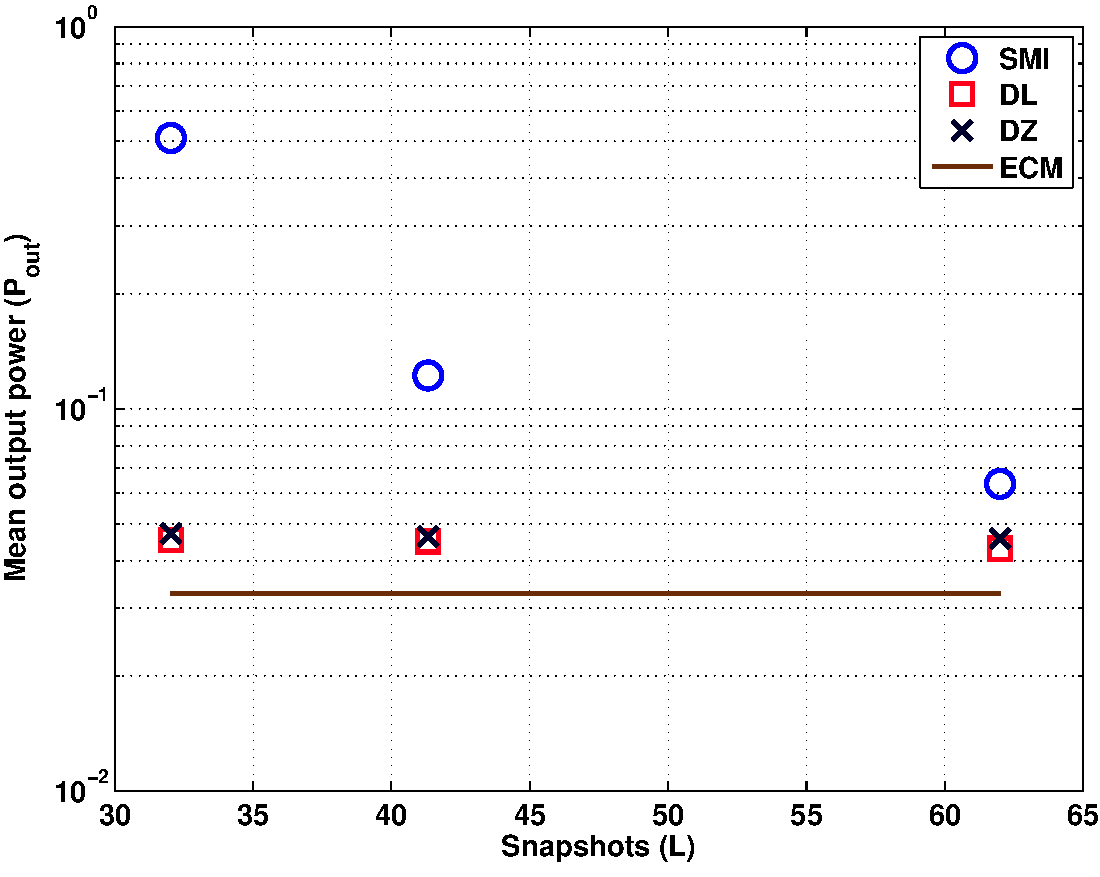
\includegraphics[width=3.5in]{pout_snapshot_N31_single.pdf}
\label{fig:pout-snapshot-L32}}
\hfil
\subfloat[Multiple interferers]{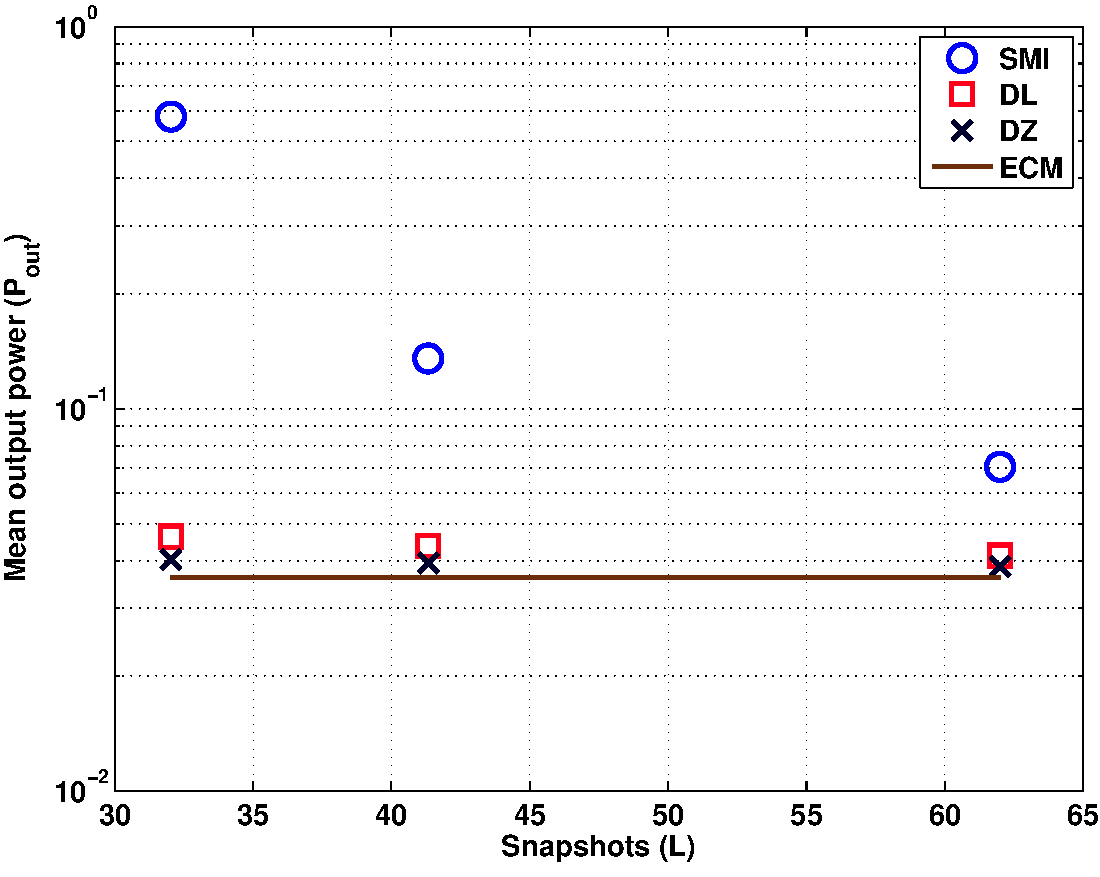
\includegraphics[width=3.5in]{pout_snapshot_N31_multi.pdf}
\label{fig:pout-snapshot-L62}}
\caption{Mean output power from ABFs using different number of
  snapshots for single and multiple interferer cases. The DZ MVDR ABF
  exhibits significant gain over the SMI MVDR ABF in suppressing
  output power when snapshot limited. The DZ MVDR ABF has a mean output
  power comparable with the DL MVDR ABF.}
\label{fig:pout-snapshot}
\end{figure*}

% The inherent subarray processing involved in implementing the DZ MVDR
% ABF widens the main lobe width and limits the degree-of-freedom
% available to suppress interferers to $(N - 1)/2$. But the results
% above indicate that the DZ MVDR ABF is still capable of reducing the 
% output power in presence of multiple interferers compared to the
% traditional SMI MVDR ABF. The consequences of subarray processing is
% further minimized in underwater applications where it is
% common to use long ULAs with hundreds of sensors
% \cite{baggeroer1999passive}. 

\subsection{Moving interferer case} 
\label{sec:moving-interferer}
This section presents results from numerical experiments evaluating
the performance of the ABFs in a moving interferer scenario. The
experiment assumes a scenario containing single spatially moving
interferer in a white background noise similarly to the
example in \cite[Sec. 4]{cox2000mrabf}. The interferer is initially at
direction $u_0 = 5/N$ and moves away from the main lobe at a constant
rate of $\rho_u$ per snapshot. The interferer direction at the
$l^{th}$ snapshot index is $u_l = u_0 + (l-1) \rho_u $ for
$l = 1, \ldots, L$ and $\rep_l = \rep(u_l)$ is the array manifold
vector for the $l\nth$ snapshot. During the snapshot averaging
interval ($l = 1,\ldots, L$), the interferer traverses some fraction
($\mu$) of the ULA resolution width, i.e.,
$\mu = \rho_u (L-1)(N - 1)/2$.

The results compare the output power of the ABFs for
varying interferer velocity cases. In each velocity case, same
number of snapshots $L = 32$ are used to estimate the SCM and compute
the weight vector ($\wthat$) for each ABF. The experiment assumes an
inbred processing approach, where the ABF weights are applied to the
same data used to compute the weights \cite{cox2002adaptive}. Several
other approaches exist for processing data in a non-stationary
environment. However, in order to make a fair comparison between the
ABFs, the experiment uses one consistent approach for all of the ABFs
compared.

In order to evaluate the ABF's output power in the moving interferer
scenario, define a `time averaged' ECM
\begin{align}
  \label{eq:time-avg-ecm}
  \avgCov &= (\interfpow/L)\sum_{l = 1}^{L}\rep_l\rep_l^H +
            \noisepow\eye  \nonumber \\ 
  &= \interfpow\repmat_L\repmat_L\herm + \noisepow\eye,
\end{align}
where $\repmat_L$ is an $N\times L$ matrix of $L$ array manifold
vectors corresponding to the interferer direction $u_l$ at each
snapshot index $l$. The `time averaged' ECM defined in
\eqref{eq:time-avg-ecm} is equivalent to an ECM corresponding to a
scenario containing $L$ independent sources each in the direction $u_l$
with power $\interfpow/L$. This scenario is essentially how the moving
interferer appears to the ULA over the snapshot averaging window
assuming perfect knowledge of the environment. The `time averaged'
ECM captures the interferer motion during the snapshot averaging
window of $l = 1,\ldots, L$. An MVDR beamformer implemented using the
'time averaged' ECM attempts to place a deep notch in each of the $L$
directions ($u_l$).

In the results discussed below, a single realization of the ABF output
power is evaluated as $\pout = \wthat\herm\avgCov\wthat$ where
$\wthat$ is the ABF weight vector. Using the definition of the `time
averaged' ECM in \eqref{eq:time-avg-ecm} the output power is,
\begin{align}
  \label{eq:time-avg-pout}
  \pout &= (\interfpow/L)\wthat\herm\repmat_L\repmat_L\herm\wthat + \noisepow\norm{\wthat}^2 \nonumber \\
&= \pinter + \pnoise,
\end{align}
where $\pinter$ is the output interferer power and $\pnoise$ is the
output noise power. All the results are obtained from a 3000 trial
Monte Carlo experiment assuming the moving interferer with $30$dB INR
and unit power white noise ($\noisepow = 1$). The CMT MVDR ABF is
implemented using the notch width parameter $\cmtW = \resW$.

\figurename{}~\ref{fig:moving-interf-ecdf} compares the output power
ECDF of the DZ MVDR, the CMT MVDR and the SMI MVDR ABFs for the moving
interferer scenario described above. The top panel assumes the
interferer traverses one resolution width during snapshot averaging
($\mu = 1$) and the bottom panel assumes the interferer moves two
resolution widths during snapshot averaging ($\mu = 2$). The dotted
vertical lines on both panels denote the output power from the
ensemble MVDR implemented using the `time averaged' ECM $\Cov_A$. This is the minimum output power achievable using the processing scheme of computing weights from $L$ snapshots. Comparisons
in \figurename{}~\ref{fig:pout-ecdf-mu1}, the case of $\mu = 1$, show
that the DZ MVDR ABF has higher probability of minimizing the output
power compared to the SMI MVDR ABF. The median output power of the DZ
MVDR ABF is more than eight times lower compared to the SMI MVDR ABF.
Also, the ECDF of the DZ MVDR ABF rises faster compared to the ECDF of
the SMI MVDR ABF indicating the output power of the DZ MVDR ABF
exhibits less variability than the output power of the SMI MVDR
ABF. The CMT MVDR ABF also improves performance over the SMI MVDR
ABF. But the DZ MVDR ABF still achieves lower median output power
compared to the CMT MVDR.

Comparisons in \figurename{}~\ref{fig:pout-ecdf-mu2}, the case of
$\mu = 2$, show that the DZ MVDR ABF again has higher probability of
minimizing the output power compared to both the SMI MVDR and the CMT
MVDR ABF. In this case, the interferer is moving at twice the velocity
compared to the case of $\mu = 1$. But the CMT MVDR ABF is still
implemented using the width parameter $\cmtW = 2/N$. The increased
interferer velocity elevates the interferer mismatch problem compared
to the case in \figurename{}~\ref{fig:pout-ecdf-mu1}. Comparing the
two velocity cases, the DZ MVDR ABF median output power increases with
the velocity while the CMT MVDR and the SMI MVDR ABFs have negligible
change in output power.

\begin{figure*}[!hp]
\centering
\subfloat[$\mu = 1$]
{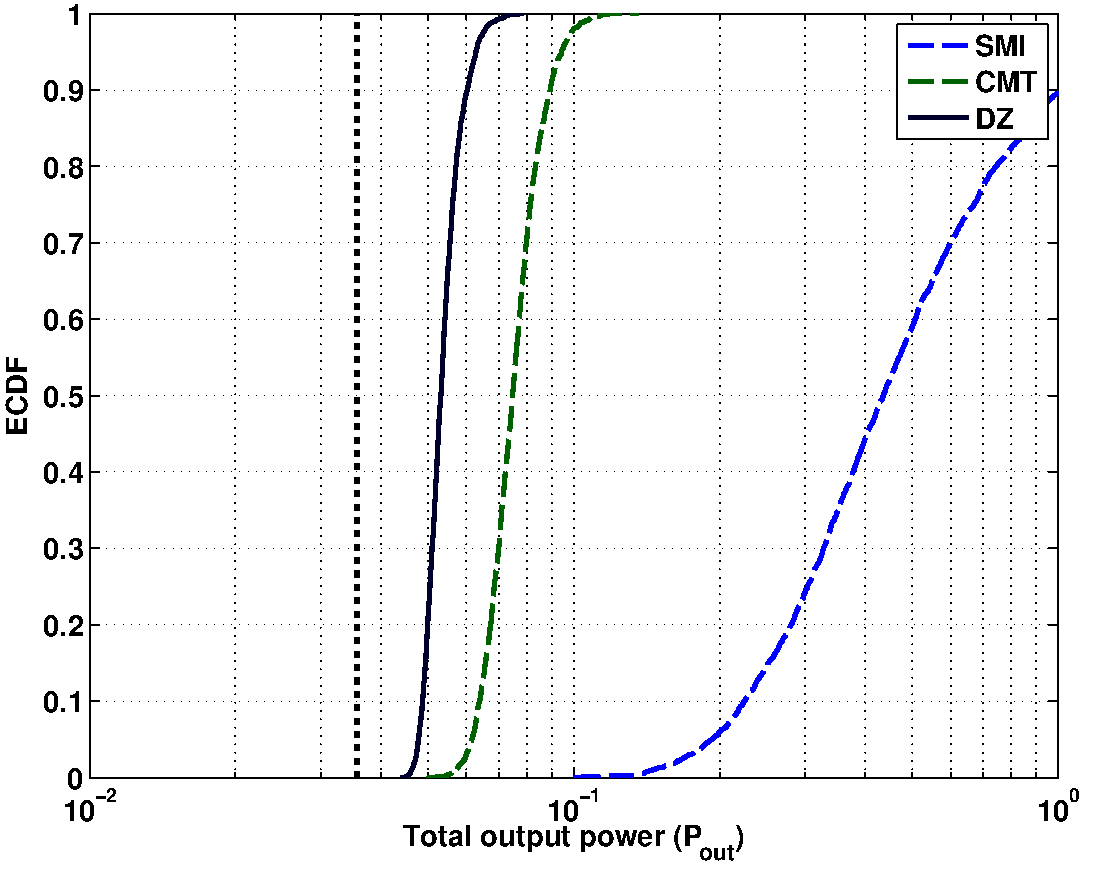
\includegraphics[width=3.5in]{dzmv_moving_interf_pout_ecdf_mu1.pdf}
\label{fig:pout-ecdf-mu1}}

\subfloat[$\mu = 2$]
{\includegraphics[width=3.5in]{dzmv_moving_interf_pout_ecdf_mu2.pdf}
\label{fig:pout-ecdf-mu2}}
\caption{Total output power ECDF for the DZ MVDR, the CMT MVDR and the
  SMI MVDR ABFs using an $N = 31$ element ULA for two interferer
  velocity cases ($\mu = 1$ and $\mu = 2$). The DZ MVDR ABF has higher
  probability of minimizing output power compared to both the SMI MVDR
  and the CMT MVDR ABF. }
\label{fig:moving-interf-ecdf}
\end{figure*}
\figurename{}~\ref{fig:varying-velocity} compares the outputs from the
DZ MVDR (black diamonds), the CMT MVDR (green squares) and the SMI
MVDR ABF (blue circles) for different interferer velocity cases.  The
top panel shows the interferer contribution to output power
($\pinter$), the middle shows the white noise contribution to output
power ($\pnoise$) and the bottom panel shows the total output power
($\pout$). Since the noise power is assumed to be unity, the noise
contribution to the output power is simply equal to the reciprocal of
the WNG as shown in \eqref{eq:time-avg-pout}.

The experiment evaluates the ABFs for cases when the interferer
traverses $\mu = \{0.5, 1, 2, 3, 4\}$ fraction of resolution width
during $L = 32$ snapshot averaging window. The interferer
contribution, the noise contribution and the total output power is
evaluated as defined in \eqref{eq:time-avg-pout} for each velocity
case. For all velocity cases, the CMT MVDR ABF is implemented with
$\cmtW = 2/N$.

\begin{figure*}[!hp]
\centering
\subfloat[Interferer output power]
{\includegraphics[width=3in]{interf_pout_diff_motion.pdf}\label{fig:interfp-diff-vel}}
\subfloat[WNG]
{\includegraphics[width=3in]{wng_diff_motion.pdf}\label{fig:wng-diff-vel}}

\subfloat[Total output power]
{\includegraphics[width=3in]{mean_pout_diff_motion.pdf}\label{fig:outp-diff-vel}}

\caption{Output from the DZ MVDR, the SMI MVDR, and the CMT MVDR ABFs
  using an $N = 31$ element ULA for varying interferer velocity
  cases. The mean output power of the DZ MVDR ABF is about $10$dB
  below the SMI MVDR ABF for all velocity cases. The mean output power
  of the DZ MVDR ABF is comparable with that of the CMT MVDR ABF.}
\label{fig:varying-velocity}
\end{figure*}


\figurename{}~\ref{fig:interfp-diff-vel} compares the mean interferer output power for each ABF at all velocity cases. Comparison shows the DZ MVDR ABF
suppresses interferers significantly better than the SMI MVDR ABF for
all velocity cases. The mean interferer output power for the DZ MVDR
ABF is more than $40$ dB below that of the SMI MVDR ABF in all
velocity cases. Comparatively, the mean interferer output power for
the CMT MVDR ABF is only about $10$ dB below that of the SMI MVDR ABF
in all velocity cases. As mentioned earlier, the DZ MVDR ABF reduces
the estimation bias of interferer eigenvectors as a consequence of
inherent subarray processing. Thus the DZ MVDR ABF is able to create
broader and deeper notch at the interferer and yield better
improvement in interferer suppression compared to the CMT MVDR ABF in
all cases of the experiment.

\figurename{}~\ref{fig:wng-diff-vel} compares the white noise
contribution to output power for each ABF at all velocity cases. The
solid horizontal line denotes the noise output power corresponding to
the optimal WNG of $N = 31$. Comparison shows that the DZ MVDR ABF has
better WNG compared to the SMI MVDR ABF and hence lower output noise
power for all velocity cases. When the interferer motion is limited
within the resolution width ($\mu \leq 1$), the DZ MVDR ABF yields
highest WNG and the lowest output noise power. At higher velocities
($\mu \geq 2$), the DZ MVDR and the CMT MVDR ABF both have comparable
output noise power. 

\figurename{}~\ref{fig:outp-diff-vel} compares the mean total output
power for each ABF at all velocity cases. The black asterisk markers
denote the output power from the ensemble MVDR implemented using the
`time averaged' ECM. The total output power is the combination of
interferer output power and the noise output power. In all velocity
cases, the contribution from the white noise dominates the total
output power for the DZ MVDR and the CMT MVDR ABFs. Both the DZ MVDR
and the CMT MVDR ABF yield significantly lower mean output power
compared to the SMI MVDR ABF in all moving interferer scenarios.
However, the CMT MVDR ABF requires choosing the notch width
parameter while the DZ MVDR ABF does not require setting a design
parameter to produce comparable performance.

\subsection{CMT MVDR ABF with multiple interferers}
\label{sec:cmt-multi-interf}
The CMT MVDR ABF with notch width $\cmtW = 2/(N-1)$ uses three degrees
of freedom (DoF) per interferer to produce broad notch as discussed in
\sect{}~\ref{sec:cmt}. The DZ MVDR ABF by design uses two DoF per
interferer. This section compares the output performance of the CMT
MVDR and the DZ MVDR ABF in case of a multiple interferers scenario.

% To compare the ABFs, consider four interferer directions $\mathbf{\uinter} = \lbrace -7/N,~7/N,~3/N,~-3/N \rbrace$. For all
% four cases, both ABFs are implemented using an $N = 31$ element ULA
% and steered towards broadside ($\ulook = 0$). The CMT MVDR ABF is implemented using notch width $\cmtW = 2/(N - 1$).

\figurename{}~\ref{fig:cmt-output-multi} compares the average output
power from the DZ MVDR (black diamonds) and the CMT MVDR ABF (green
circles) for four cases with different number of interferers
$D = 1\,\text{to}\,4$. The experiments starts with $D = 1$ interferer
at $\uinter = -7/N$ and introduces one additional interferer for each
new case. The direction for additional interferers is chosen
sequentially from the set
$\mathbf{\uinter} = \lbrace 7/N,~3/N,~-3/N \rbrace$ respectively. For
all four cases, both ABFs are implemented using an $N = 11$ element
ULA and steered towards broadside ($\ulook = 0$). The CMT MVDR ABF is
implemented using notch width $\cmtW = 2/(N - 1$). Examining the
output power, the DZ MVDR and the CMT MVDR ABF produce comparable
output for $ D \leq 2$. But for $D > 2$, the CMT MVDR ABF produces
significantly higher output power compared to the DZ MVDR ABF.
\figurename{}~\ref{fig:wng-cmt-multi} compares the inverse of the WNG
of the ABFs.  The inverse of WNG is proportional to the white noise
contribution to output power. When $D > 2$ the white noise
contribution of the CMT MVDR ABF increases significantly. In presence
of multiple interferers, the CMT MVDR ABF fails to suppress output
power as it uses more DoF per interferer compared to the DZ MVDR ABF
as discussed below.

The MVDR ABFs using $N = 11$ element ULA and steered to a fixed look
direction are limited to $N-2 = 9$ DoF for adaptation. When $D = 2$,
the CMT MVDR uses six DoF to suppress interferer and the remaining
DoFs are used for white noise suppression. But when $D = 3$, the CMT
MVDR ABF uses all nine DoF to suppress interferer leaving no DoF for
white noise suppression. This results in loss of WNG for the CMT MVDR
and subsequent increase in white noise contribution to output
power. Moreover when $D = 4$, the CMT MVDR ABF requires more than nine
DoF, which results in failure to suppress interfere and loss of
WNG. As a result the CMT MVDR ABF produces significantly high output
power. In contrast, even when $ D = 4$, the DZ MVDR uses only eight
DoF to suppress interferers. As a result the DZ MVDR ABF consistently
produces lower output power for all four interferer cases.

\begin{figure*}[!hp]
  \centering
  \subfloat[Total output power]{    \includegraphics[width=3.5in]{./cmt_multi/dz_vs_cmt_Pout_multi_case2.pdf}
    \label{fig:cmt-output-multi}}

  \subfloat[White noise contribution]{
    \includegraphics[width=3.5in]{./cmt_multi/dz_vs_cmt_wng_multi_case2.pdf}
    \label{fig:wng-cmt-multi}}
  \caption{Comparison of (a) Output power and (b) white noise
    contribution to output from the DZ MVDR and the CMT MVDR ABFs for
    different number of interferers. Both ABFs are implemented using
    $N = 11$ sensor ULA and steered towards broadside. The CMT MVDR
    uses notch width of $\cmtW = 2/(N-1)$. As the number of
    interferers increases, the CMT MVDR fails to suppress output power
    as it uses more DoF per interferer compared to the DZ MVDR ABF.}  
\end{figure*}

% As previously mentioned, the DZ MVDR ABF has only $(N-1)/2$ degrees of
% freedom (DoF) for interferer suppression. Equivalently the DZ MVDR
% polynomial has only $(N-1)/2$ unique zeros for interferer
% suppression. On the other hand, the CMT MVDR ABF using full ULA has
% $(N - 1$) DoF for interferer suppression. Equivalently the CMT MVDR
% polynomial has $N-1$ zeros for interferer suppression. However, as
% mentioned in \sect{}\ref{sec:cmt}, depending on the notch width, the
% CMT MVDR ABF uses multiple zeros per interferer to produce broad notch
% which reduces the effective DoF available for interferer
% suppression. As the number of interferers increases more zeros are
% used for notch broadening and fewer zeros are available for the white
% noise suppression.

% \figurename{}~\ref{fig:cmt-zeros-multi} shows a representative example
% of DZ MVDR polynomial zeros (black) and the CMT MVDR polynomial zeros
% (green). For simplicity, the example uses $N = 11$ element ULA. The
% dotted radial lines indicated the four interferer directions
% $\mathbf{\uinter} = [-7/N,~7/N,~3/N,~-3/N]$ considered in
% \figurename{}~\ref{fig:cmt-output-multi}. The DZ MVDR ABF places a SOZ
% in the vicinity of each interferer direction to produce broad
% notches. Comparatively, the CMT MVDR ABF places up to three zeros in
% the vicinity of the interferer directions. As a result, all ten of CMT
% MVDR polynomial zeros are used to produce wide notches for merely
% $D = 4$ interferers. The clustering of all zeros in the interferer
% direction yields high sidelobes in between the broad notches. The high
% sidelobes in CMT MVDR beampattern lead to significant loss of the WNG
% and subsequent rise in output power. Since the number of zeros used
% per interferer depends on the choice of the notch width ($\cmtW$), it
% is imperative for the CMT MVDR ABF to use suitable value of
% $\cmtW$. However, the DZ MVDR ABF does not require choosing a design
% parameter and consistently suppresses output power for $D < (N -1)/2$.

% \figurename{}~\ref{fig:cmt-zeros-multi} shows the polynomial zeros for the CMT MVDR (green circles) and the DZ MVDR (black diamonds). The left panel considers the case of $D = 3$ interferers and the right panel considers the case of $D = 4$ interferers. 

% \begin{figure*}[!hp]
%   \centering
%   \subfloat[D = 3]{
%     \includegraphics[width=3in]{./cmt_multi/cmt_pzplot_multi_D3.pdf}}
%   \subfloat[D = 4]{
%     \includegraphics[width=3in]{./cmt_multi/cmt_pzplot_multi_D4.pdf}}
%   \caption{Zeros of CMT MVDR polynomial (green circles) and DZ MVDR
%     polynomial (black diamonds). The CMT MVDR ABF uses multiple zeros
%     at each interferer direction, depending on the chosen notch
%     width. The DZ MVDR ABF always uses two zero per interferer.}
% \label{fig:cmt-zeros-multi}
% \end{figure*}

% The
% DZ MVDR ABF consistently achieves lower output power under same
% conditions as observed in \figurename{}~\ref{fig:cmt-output-multi}.



% % Make clear that L snapshots are used to compute the weights first. Then we look at the output power over the same interval using the ECM for each instance.

% \subsection{Computational gain}
% \label{sec:computational-gain}
% \figurename{}\ref{fig:comp-gain} compares the computation time
% required by DZ MVDR (diamond markers) and SMI MVDR ABF (circle
% markers) implemented using ULAs with number of sensors ranging from
% $N = 11$ to $101$. The computation time for each ULA size was averaged
% over 3000 Monte Carlo experiments. Each experiment assumed $L = 2N$
% snapshots were available to implement the ABFs. DZ MVDR ABF clearly
% requires less computation time compared to the SMI MVDR ABF. The gain
% is more significant for longer arrays.

% % TODO: Consider including comp time for UC DZ MVDR to show that it
% % takes up more time than SMI MVDR.

% \begin{figure}[!t]
%   \centering
%   \includegraphics[width=2.5in]{comp_gain.pdf}
%   \caption{Computational gain using DZ MVDR over SMI MVDR.}
%   \label{fig:comp-gain}
% \end{figure}

%%% Local Variables:
%%% mode: latex
%%% TeX-master: "main"
%%% End:
  % result discussion
% ==========================================

\section{Summary}
\label{sec:dzmvdr-summary}
In conclusion, this chapter presents the DZ MVDR ABF which produces
a broad notch in the beampattern in the interferer direction. The DZ
MVDR ABF doubles the array polynomial zeros of a subarray SMI MVDR ABF
to derive the weight vector. The DZ MVDR ABF with the inherent
subarray processing requires less computation compared to the SMI MVDR
ABF implemented using same sized ULA. But the gain from subarray
processing is at the cost of reduced DOF and a wider main-lobe than the
SMI MVDR or the DL MVDR ABFs. Numerical experiments show that the DZ
MVDR ABF suppresses interferers better than both the SMI MVDR and the
DL MVDR ABF in the multiple stationary interferer scenario. Comparison
of the WNG shows that on average the DZ MVDR ABF has higher WNG making
it less sensitive to parameter mismatch. In moving interferer
scenarios, the DZ MVDR ABF performance is comparable to the CMT MVDR
ABF with the width parameter set equal to the ULA resolution
width. But the CMT MVDR requires choosing the width parameter while
the DZ MVDR ABF does not require making prior choice of design
parameters.

%%% Local Variables: 
%%% mode: latex
%%% TeX-master: "main"
%%% End: 
  % Everything on UC MVDR algorithm

\chapter{Conclusions}
\label{ch:conclusion}
The work presented in this thesis develops a model for the ensemble
zero locations and introduces two new ABF algorithms. The model for
the ensemble zeros expresses the zero locations as a function of the
INR. The model highlights the trade off between the interferer
suppression and white noise gain to produce minimum output power using
the ensemble MVDR beamformer. Numerical evaluation show that the model
predictions are a good match to the ensemble zero location, for a
range of INR values.

The UC MVDR ABF introduced in Ch.~\ref{ch:ucmvdr} improves interferer
and white noise suppression of the SMI MVDR ABF. The UC MVDR algorithm
moves the sample zeros radially to the unit circle satisfying the unit
circle constraint on the ensemble zeros. The UC MVDR approach differs
from the diagonal loading approach which is shown to move the sample
zeros along specific trajectories towards the CBF zero
locations. Simulation results show that the UC MVDR ABF yields deeper
notch at the interferer direction and improves WNG performance
compared to the SMI MVDR ABF, and the DL MVDR ABF with comparable DL
factor. Additionally, implementation of the UC MVDR in a snapshot deficient case and the unit circle DMR ABF are also discussed.

The DZ MVDR ABF introduced in Ch.~\ref{ch:dzmvdr} is a new approach to
notch broadening. The proposed algorithm exploits the property of ABF
beampattern near a second-order zero combined with subarray processing
to produce broad notches at interferer directions. Numerical
simulations evaluated the performance of the DZ MVDR ABF in presence
of stationary and moving interferers. The eigenanalysis of the sinc
taper matrix reveled that the CMT MVDR uses three DoFs per interferer
when the notch width is set equal to one resolution
width. Consequently, in presence of multiple interferers, the CMT MVDR
failed to suppress output power compared to the DZ MVDR ABF which uses
only two DoF per interferer.

%%% Local Variables:
%%% mode: latex
%%% TeX-master: "main"
%%% End:


% ---------- End of Chapters----------------------------------
% % Back matter
% \e{IEEEexample:BSTcontrol}
%\appendix
%\addappheadtotoc
%\appendixpage
%\appendixpageoff
\begin{appendices}
\addtocontents{toc}{\def\protect\cftchappresnum{Appendix }}
\addtocontents{toc}{\addtolength\cftchapnumwidth{\widthof{ix }}}
\chapter{Proof of unit circle constraint on MVDR zeros}
\label{sec:apdx-mvdr-zeros}
The ensemble MVDR polynomial zeros are constrained to fall on the unit circle
for planewave beamforming using a ULA. Steinhardt and Guerci proved this
constraint on the MVDR ensemble zeros in \cite{steinhardt2004stap},
but the result does not appear to be widely known. The proof below
closely follows the Steinhardt and Guerci's proof by contradiction.

The ensemble MVDR weight vector $\wmvdr$ solves the optimization problem in
\eqref{eq:mvdr-const-prob}. The quadratic objective function in
\eqref{eq:mvdr-const-prob} is a convex function in $\wt$ because the
ECM is a positive-definite matrix \cite{vtree2002oap}. This implies a
unique solution exists for \eqref{eq:mvdr-const-prob}. Using the Parseval's relation (\cite[Sec.~5.4.1.3]{vtree2002oap}), the objective
function can be expressed in terms of the ensemble input power spectrum
$\powspec$ and the ensemble MVDR beampattern
\begin{equation}
\label{eq:obj-func-spec}
f(\wt) = \half\int_{-1}^{1}\powspec |\beampatu|^2 \,du.
\end{equation}
Replace the beampattern with the array polynomial
${P(z = e^{j\pi u})}$ to get
\begin{equation}
\label{eq:obj-func-poly}
f(\wt) = \half\int_{-1}^{1}\powspec |P(e^{j\pi u})|^2 \,du.
\end{equation}

Assume the weight vector $\wmvdr$ solves the optimization problem \eqref{eq:mvdr-const-prob}. The ensemble zero locations correspond to the ensemble MVDR weight vector. Factor the polynomial $P(e^{j\pi u})$ in terms of ensemble zeros
\begin{equation}
  \label{eq:mvdr-poly-zeros-format}
P(e^{j\pi u}) = \prod\limits_{n=1}^{N-1}\frac{(1 - \ensz_i e^{-j\pi u})}{(1 - \ensz_i)},
\end{equation}
where $\ensz_i$s are the ensemble zeros and $P(z) = 1$ for
$z = 1$.
Using \eqref{eq:mvdr-poly-zeros-format} in \eqref{eq:obj-func-spec},
the objective function is
\begin{equation}
\label{eq:obj-func-zeros-form}
f(\wmvdr) = \half\int_{-1}^{1}\powspec \prod\limits_{n=1}^{N-1}\frac{(1 -
   \ensz_n e^{-j\pi u})}{(1 - \ensz_n)} \frac{(1 - \ensz_n^*e^{j\pi u})}{(1 - \ensz_n^*)}\,du
\end{equation}
Assume the zeros in \eqref{eq:mvdr-poly-zeros-format} are not on the
unit circle. Replacing one zero $\ensz_i$ by its conjugate-reciprocal
$1/\ensz_i^*$ in \eqref{eq:obj-func-zeros-form} keeps the objective
function unchanged. However, changing the zero alters the polynomial resulting in a
different weight vector. This implies there exists a weight vector
different from the weight vector corresponding to
\eqref{eq:mvdr-poly-zeros-format} which still optimizes
\eqref{eq:mvdr-const-prob}. This contradicts with the uniqueness of
the solution to \eqref{eq:mvdr-const-prob}. The uniqueness holds only
when the zeros of $\mvdrpoly{z}$ are on the unit circle. Hence the MVDR
zeros must be on the unit circle.

% =====================================================================

\chapter{Evaluation of derivatives}
\label{app:apdx-derivation}
In \sect{}\ref{sec:perturbation-model}, solving for the optimal phase angle perturbation parameter $\deltau$ requires evaluating the derivatives in \eqref{eq:derivative-equation}. This appendix presents the evaluation of the expression for the derivatives.

Using the definition in \eqref{eq:approx-inter-pout}, the derivative of the interferer contribution to the output power is 
\begin{align} 
 \label{eq:inter-pout-derivative}
 \frac{d\,P_I(\deltau)}{d\deltau} =& \interfpow|\cbfNtwozeropoly(\uinter)|^2 \frac{d |\funczero{\expo{j\pi \uinter}}|^2}{d\deltau}.
\end{align}
Using the definition in \eqref{eq:approx-wn-pout} the derivative of the white noise contribution to the output power is
\begin{align}
\label{eq:wn-pout-derivative}
\frac{d\,P_W(\deltau)}{d\deltau} =& \frac{\noisepow}{2}\int\limits_{-1}^{1} |\cbfNtwozeropoly(u)|^2 \frac{d|\funczero{\expo{j\pi \uinter}} |^2}{d\deltau}\,du.
\end{align}
Eq.~\eqref{eq:wn-pout-derivative} used the Leibniz integral rule to simplify the derivative of the integral. 
Evaluating \eqref{eq:inter-pout-derivative} and \eqref{eq:wn-pout-derivative} requires the derivative of $|\funczero{\expo{j\pi u}}|^2$ w.r.t.  $\deltau$. Using the expression for $|\funczero{\expo{j\pi u}}|^2$ from \eqref{eq:bp-poly-perturb}, the derivative is
\begin{align} 
\label{eq:funczero-derivative}
\frac{d\, |\funczero{\expo{j\pi u}}|^2}{d\deltau} =& \frac{-(\sin(a) + \sin(b) - \sin(a+b))}{(1 - \cos(b + \pi\deltau))^2} + \nonumber \\
& \frac{(\cos(a) - \cos(b))\pi\deltau}{(1 - \cos(b + \pi\deltau))^2} 
\end{align}
where $a = \pi(u - \uinter)$, $b = \pi\uinter$. In the region of INR
$>10$dB in \figurename{}~\ref{fig:mvdr-zeros-phase}, the perturbation
angle $\deltau$ is very small as indicated by an almost flat solid
black curve aligned against the dashed horizontal line. The subsequent
derivation uses the following the small angle approximations
$\sin(\pi\deltau) \approx \pi\deltau$ and
$\cos(\pi\deltau) \approx 1$. Substituting
\eqref{eq:funczero-derivative} in \eqref{eq:inter-pout-derivative}
gives
\begin{align} 
\label{eq:nd-derivative}
\frac{d\,P_I(\uinter, \deltau)}{d\deltau} =& \interfpow |\cbfNtwozeropoly(\uinter)|^2 \frac{\pi\deltau(1 - \cos(\pi\uinter))}{(1 - \cos(b + \pi\deltau))^2} \nonumber \\
=& \interfpow\frac{\pi\deltau C}{(1 - \cos(b + \pi\deltau)},
\end{align}
and substituting in \eqref{eq:wn-pout-derivative} gives
\begin{align} 
\label{eq:wng-derivative}
\frac{d\,P_W(u, \deltau) }{d\deltau} =& \noisepow \biggl(\half\int_{-1}^{1} \
\frac{-|\cbfNtwozeropoly(u)|^2(\sin(a) + \sin(b) - \sin(a+b))}{(1 - \cos(b + \pi\deltau))^2}\, du + \nonumber\\
& \frac{\pi\deltau}{2}\int_{-1}^{1} \frac{|\cbfNtwozeropoly(u)|^2(\cos(a)-\cos(b))\pi\deltau}{(1 - \cos(b + \pi\deltau))^2} \, du \biggr)  \nonumber \\
=& \frac{\noisepow(-A + \pi\deltau B)}{(1 - \cos(b + \pi\deltau)}
\end{align}
where constants $A$, $B$ and $C$ are
\begin{align*}
  A =& \half\int_{-1}^{1} \
     |\cbfNtwozeropoly(u)|^2(\sin(a) + \sin(b) + \sin(a+b))\, du \\
  B =& \half\int_{-1}^{1} |\cbfNtwozeropoly(u)|^2(\cos(a)-\cos(b))\pi\deltau \, du \\
  C =& |\cbfNtwozeropoly(\uinter)|^2\pi\deltau(1 - \cos(\pi\uinter)).
\end{align*}

Using \eqref{eq:nd-derivative} and \eqref{eq:wng-derivative} in \eqref{eq:derivative-equation} gives
\begin{align}
  \label{eq:1}
  -\interfpow \pi\deltau C &=  \noisepow (-A + \pi\deltau B)
\end{align}

%%% Local Variables:
%%% mode: latex
%%% TeX-master: "main"
%%% End:
  
\end{appendices}

\clearpage
\addcontentsline{toc}{chapter}{Bibliography}
\bibliographystyle{../refs/IEEEtran}

\bibliography{../refs/IEEEabrv,../refs/myrefs}

\end{document}

%%% Local Variables:
%%% mode: latex
%%% TeX-master: "main"
%%% End:

